%
%        LATEX SOURCE FOR JOURNAL OF NEUROSCIENCE RESUBMISSION
%
% INSTRUCTIONS
% ============
%
%-  Using filecontents package to inline the bibliography.
%
% - Compile (on Linux) with the following commands:
%
%          pdflatex JoN-resubmission
%          bibtex -min-crossrefs=99999 JoN-resubmission
%          pdflatex JoN-resubmission
%          bibtex -min-crossrefs=99999 JoN-resubmission
%          pdflatex JoN-resubmission
%          pdflatex JoN-resubmission
%
% - Figures declared where they should appear in the text. They may all be
%   moved to end of the document if necessary.
%
% - Originally used the 'namedplus' bibliography style:
%   (http://homepages.inf.ed.ac.uk/mhennig/bibtex/)
%   for compatibility with Journal of Neuroscience guidelines.
%   Switched to natbib and apalike for resubmission.
%
% - Title page and Acknowledgment need to be moved as appropriate.

 \documentclass{article}

%\usepackage{setspace}
%\doublespacing

\usepackage{graphicx}
\usepackage{amsmath}

\usepackage{mathptmx}       % selects Times Roman as basic font
\usepackage{helvet}         % selects Helvetica as sans-serif font
\usepackage{courier}        % selects Courier as typewriter font

\usepackage[margin=1.0in]{geometry}
\usepackage[cdot,mediumqspace,squaren,Gray]{SIunits}

\usepackage{natbib}        % Originally used namedplus package.
\usepackage{filecontents}  % Inline bibliography as not allowed to submit .bib file.

%==============%
% Figure sizes %
%==============%

\def \scalefactor {0.666666}
\def \chapmanScale {\scalefactor}          % 2 column
\def \schematicScale {\scalefactor}        % max. 1.5 column
\def \metricScale {\scalefactor}           % 2 column
\def \LdevelopmentScale {\scalefactor}     % 2 column
\def \GaussianScale {\scalefactor}         % 2 column
\def \NoisytoNaturalScale {\scalefactor}   % 2 column
\def \GRScale {\scalefactor}               % 2 column
\def \ORTuningScale {\scalefactor}         % 2 column


\begin{document}

\begin{titlepage}


\title{Mechanisms for stable, robust, and adaptive development of
  orientation maps in the primary visual cortex\\
{\large Journal of Neuroscience (2013), in press.}
}
\author{Jean-Luc R. Stevens$^1$ (jlstevens@ed.ac.uk), Judith S. Law$^1$ (jkirkwoodlaw@gmail.com),\\
Jan Antolik$^{1,2}$ (antolik@unic.cnrs-gif.fr), and James A. Bednar$^1$ (jbednar@inf.ed.ac.uk)}
\maketitle

\noindent
$^1$ Institute for Adaptive and Neural Computation, University of Edinburgh, EH8 9AB, UK\\
$^2$ Unit{\'e} de Neuroscience, Information et Complexit{\'e}, CNRS, Gif sur Yvette, France.\\

\noindent


\section*{Acknowledgments}
This work was supported in part by grants EP/F500385/1 and
BB/F529254/1 to the University of Edinburgh Doctoral Training Centre
in Neuroinformatics and Computational Neuroscience (www.anc.ed.ac.uk/dtc)
from the UK EPSRC, BBSRC, and MRC research councils.  The work has
made use of resources provided by the Edinburgh Compute and Data
Facility (ECDF; www.ecdf.ed.ac.uk).  Thanks to Philipp Rudiger, Chris
Ball, Stuart Wilson and other members of the Institute for Adaptive
and Neural Computation for helpful comments and discussion. This work
is dedicated to the memory of Barbara Chapman, 1963-2013.

\end{titlepage}


\begin{abstract}
Development of orientation maps in ferret and cat primary visual
cortex (V1) has been shown to be \emph{stable}, in that the earliest
measurable maps are similar in form to the eventual adult map,
\emph{robust}, in that similar maps develop in both dark rearing and
in a variety of normal visual environments, and yet \emph{adaptive},
in that the final map pattern reflects the statistics of the specific
visual environment.  How can these three properties be reconciled?
Using mechanistic models of the development of neural connectivity in
V1, we show for the first time that realistic stable, robust, and adaptive map
development can be achieved by including two low-level mechanisms
originally motivated from single-neuron results.  Specifically,
contrast gain control in the retinal ganglion cells and the lateral
geniculate nucleus reduces variation in the presynaptic drive
due to differences in input patterns, while homeostatic plasticity of
V1 neuron excitability reduces the postsynaptic variability in firing
rates.  Together these two mechanisms, thought to be applicable across
sensory systems in general, lead to biological maps that
develop stably and robustly, yet adapt to the visual environment.  The
modeling results suggest that topographic map stability is a natural
outcome of low-level processes of adaptation and normalization.  The
resulting model is more realistic, simpler, far more robust, and
is thus a good starting point for future studies of cortical map
development.
\end{abstract}

\section{Introduction}

% jbednar: awk
Orientation-selective neurons in carnivoran and primate primary visual
cortex (V1) form systematic topographic maps organized by preferred
retinal location and orientation
\citep{Blasdel1992a,Blasde1992b,Kaschube2010}.  Optical imaging
studies in ferrets indicate that these orientation maps develop in a
stable way, with a high similarity
in the spatial layout between the weakly selective
initial maps and the final highly selective configuration
(\citealp{Chapman1996,Chapman1998,Godecke1997}; see figure
\ref{fig:ferret_stability}).  This stability
may be important for allowing regions downstream
from V1 to develop, and is particularly remarkable given that
V1 neurons undergo massive morphological changes over this
time (reviewed by \citealp{White2007,Huberman2008}).  V1 map
development is also
quite robust against differences in inputs, with similar final map
patterns developing until nearly three weeks of age in cats,
irrespective of whether the eyes are open \citep{Crair1998}.  Yet map
development is not simply decoupled from vision, because
the development of selectivity corresponds to a
\emph{critical period} during which visual experience is required for
neurons to achieve fully mature levels of orientation tuning
\citep{White2007,White2001b,Crair1998,chapman:jn00}. Moreover,
neurons and maps in animals reared in abnormal visual conditions during the
critical period come to reflect the statistics of the abnormal visual
input (e.g.\ lid suture , \citep{Blakemore1975,White2001b,wiesel:jnp63},
striped environments \citep{Blakemore1970,Sengpiel1999},
or oriented blurring via goggle
rearing \citep{Tanaka2006,Tanaka2009}).

Together, these results indicate that orientation map and selectivity
development is remarkably stable and robust against variability in
inputs over time or across animals, yet adaptive to the statistics of
available visual input.  Although numerous computational models of
activity-driven map development have been proposed (reviewed by
\citealp{Swindale1996,goodhill:neuron07}), no map model has yet been
shown to develop stably in response to patterned inputs of different
types and strengths.  Understanding how maps can develop stably is
both of direct scientific interest, and may provide a criterion that
allows inherently unstable models to be rejected.

In this paper, we begin with a simple mechanistic model including
lateral connectivity that captures the essential features of previous
incremental Hebbian self-organizing network models for map development
\citep{vondermalsburg:selforg,kohonen:original,Obermayer1990,Sirosh1994a,barrow:nc96,Burger1999,Burger2001,bednar:neurocomputing04-or,Miikkulainen2005},
while omitting mechanisms that destroy stability. Although this model
develops maps, we show that it is still relatively unstable, and is
not robust to changing inputs, e.g.\ varying input contrast. We then
demonstrate that extending the model with two well-established
low-level properties, neuron threshold adaptation and feed-forward
gain control, independently improves robustness and stability, and
that when used together the final GCAL (Gain Control, Adaptation,
Laterally connected) model achieves biological maps with robust and
stable development, while reflecting the statistics of visual input.
The results suggest that the well-established mechanisms of gain
control and single-neuron homeostatic adaptation are important basic
principles underlying map development, not just for individual adult
or developing neurons.
%%
\begin{figure}
\centerline{
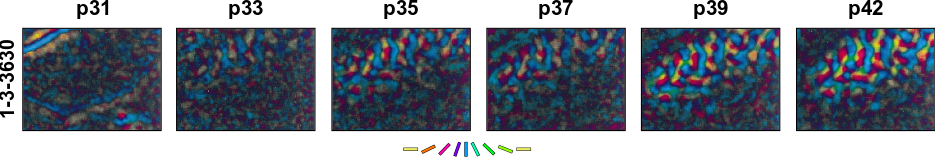
\includegraphics[scale=\chapmanScale]{./figures/fig01.pdf}
}

\caption[]{{\bf Stable development of orientation maps in ferret
    striate cortex.} Orientation maps recorded in the primary visual
  cortex of one ferret (animal 1-3-3630) at the postnatal age
  indicated above. In these polar maps, pixel color indicates
  orientation preference and pixel brightness indicates the strength
  of orientation tuning. The selectivity of each map is normalized
  independently, making blood vessels visible at p31 (e.g.\ the blue
  streak in top-left corner) but not at p42 once orientation
  selectivity has developed.  As the maps mature, iso-orientation
  domains become visible as colored regions that become more strongly
  responsive over time, without changing the overall map pattern.
  Data reproduced from \citealt{Chapman1996}.}
\label{fig:ferret_stability}
\end{figure}

\section{Materials and Methods}
\small

The following sections first present methods used for quantifying the
emergence of selectivity in biological maps, the stability of these maps over
time, and the degree to which model maps resemble biological maps. We then
describe the set of models used in this paper.

\subsection*{Measuring stability and selectivity}

%%
  Stability and selectivity measures for maps obtained by
  \citet{Chapman1996} using optical imaging in eight ferrets (of
  either sex; personal communication, Tobias Bonhoeffer) are shown in
  figure \ref{fig:chapman} and described below.%%
%%
\begin{figure}
\centerline{
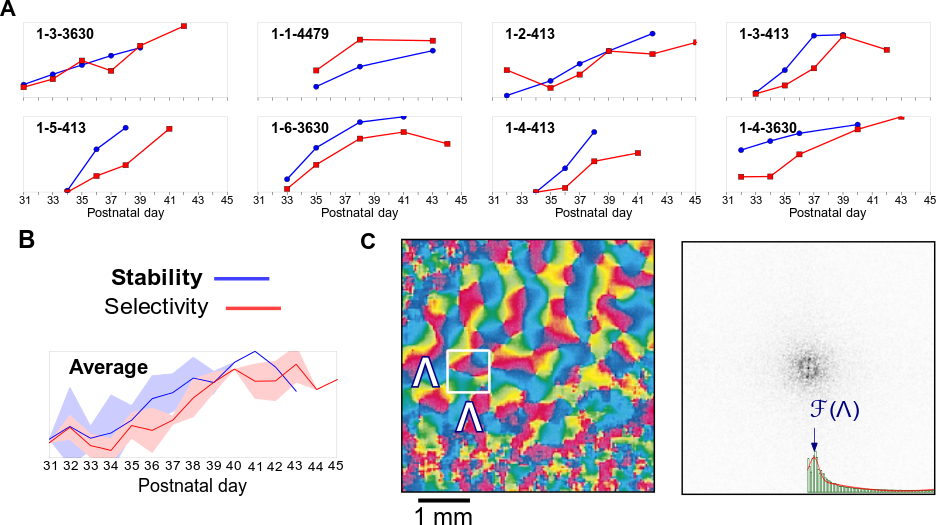
\includegraphics[scale=\chapmanScale]{./figures/fig02.pdf}
}
\caption[]{\textbf{Development of orientation maps measured by chronic
    optical imaging in ferrets.}  (A) Recorded selectivity (red square
  markers) and stability values (blue round markers) for all eight
  ferrets, as a function of postnatal day (replots data from
  \citet{Chapman1996} figures 4 and 7).  Stability is quantified by
  the average difference in preference of each
  orientation map with the final map, as defined by
  equation~\ref{eqn:similarityindex}.  A common selectivity and
  stability scale is used to allow comparison between ferrets. All
  values are in arbitrary normalized units, using the lowest recorded
  value as the zero reference point, and the highest recorded value as
  the maximum (see Methods). (B) The mean selectivity and stability
  across ferrets as a function of postnatal day, with the $\pm$95\%
  confidence intervals for each day indicated by the shaded area
  around the mean line. Selectivity and stability increase steadily
  and simultaneously over development so that once neurons are
  selective, they are organized into a map with the same form as the
  final measured map. These results show that selectivity does not precede increasing
  stability, indicating stable map development.
  (C) As a reference for later modelling work, the final orientation
  preference map (without selectivity) for ferret 1-3-360 on day P42
  (rightmost plot in figure~\ref{fig:ferret_stability}) is shown.  The
  map is organised into regularly repeating hypercolumns in all
  directions, as seen by the ringness in the Fourier power spectrum,
  plotted with the highest amplitude component in black.
  The center value is the DC component and the midpoint of each edge
  represents half of the highest possible spatial frequency
  in the cardinal directions  (i.e.\ the Nyquist frequency).
  This Fourier spectrum is used to calculate the average periodicity
  of the map, which is then plotted as a hypercolumn area $\Lambda^2$,
  covering one period in the cardinal directions.
  Figure~\ref{fig:metric} illustrates how to use these
  calculations to determine if a model map resembles this animal data.
}
\label{fig:chapman}
\end{figure}

  Qualitatively, map development is considered stable if the map
  pattern remains constant once neurons have become highly selective;
  unstable development would be characterized by maps that reorganize
  substantially after orientation-selective patches first emerge
  \citep{Chapman1996}.
  %%
  In electrophysiological measurements from ferret V1, average
  selectivity (orientation tuning) is low from about postnatal day 23
  (P23; when visual responses can first be measured) until P28--P34,
  reaching adult levels by P42--P49 \citep{Chapman1993}.  To examine
  stability of maps using optical imaging, \citet{Chapman1996} thus
  focused on the period from P31 to P45.  This period also corresponds
  to the critical period for visual experience---disrupting activity
  before P50 eliminates selectivity even with normal visual experience
  after this age \citep{chapman:jn00}.  For this modelling study,
  we will also focus on this period of normal orientation selectivity
  emergence; stability after the critical period can be modelled
  trivially by disabling or greatly reducing plasticity, and will not
  be investigated further here.

  The red lines with square markers in figure \ref{fig:chapman}A show
  the average selectivity of the optical imaging signal from P31-P45
  for all eight ferrets \citep{Chapman1996}; one additional datapoint
  from ferret 1-1-4479 at P55 is not shown. Although the selectivity
  values are on an arbitrary scale due to the measurement technique,
  the values for each postnatal age correspond closely to those found
  electrophysiologically \citep{Chapman1996}, and thus cover the range
  from highly unselective to adult-like selectivity.

To assess stability quantitatively over this same time period,
\citet{Chapman1996} computed the
correlation of orientation preference at each developmental age with
the organized preference map observed in the final recording for that
animal.  For convenience, we have linearly rescaled the ``orientation
similarity index'' values from that study to vary from 0.0
(uncorrelated preference) to 1.0 (identical preference), which we
compute as a Stability Index ($SI$):
%%
\begin{equation}
SI =1-\frac{4}{n \pi}\sum_{i}{\mid(F_{i}-O_{i})~\mbox{mod}~\left(\frac{\pi}{2}\right) \mid},
\label{eqn:similarityindex}
\end{equation}
%%
where $i$ iterates over all $n$ datapoints (pixels in the imaging
frame), $F_i$ is the final orientation preference value for the
neural unit corresponding to pixel $i$, and $O_i$ is the corresponding preference value at an earlier
age.  The blue lines with round markers in figure \ref{fig:chapman}A
show the results of this calculation for eight ferrets from
\citet{Chapman1996} measured at different postnatal days.
Note that even identical underlying maps would give values below
1.0 on this measure, if there is any noise or variation in measuring
the map, and so the values shown have been normalized by the highest and
lowest stability values across all ferrets studied.

Given this data, stable development is defined as a map having high SI
index values whenever the average selectivity value is high.  When the
selectivity is very low, presumably before the neurons have developed
at all, the map is arbitrary and dominated by measurement noise, but
if development is stable the SI value should increase as soon as the
selectivity value increases.  Unstable development would be visible as
a selectivity value that increases well before stability does,
representing neurons that have achieved selectivity before assuming
the final preference value observed in the last map measured.  As can be seen in
\ref{fig:chapman}A, the SI value and the average selectivity are
highly correlated in every ferret shown, with both values typically
increasing over time rather than selectivity predating stability
(though ferret 1-1-4479 could be seen as relatively unstable).  An
overall correlation between selectivity and stability is a hallmark of
stable map development, and is visible as a general trend in the average data from all ferrets, plotted in
\ref{fig:chapman}B.

\subsection*{Assessing the organization of orientation maps}

Recording the selectivity and stability index is sufficient for
evaluating development in experimental recordings, where all maps are
necessarily biologically realistic. In simulated models
of map development, there 
is no guarantee that simulated maps have an orientation structure
matching those observed in real animals. An unrealistic map may be
both stable and selective, and so we require that a good model of map
formation also results in realistic maps, similar to those
found in animals. Ideally, map quality would be assessed with an
automated metric that reports how close the maps are to animal data,
e.g.\ on a scale from 0 to 1.0 as for stability.

There have been several previously published
measures that could be used to quantify the degree of map
organization.  Biological maps tend to be smooth, which can be measured
by the local homogeneity index (LHI; \citealp{Nauhaus2008}) or the
earlier ``local input orientation selectivity index''
\citep{schummers:jpp04}, which both convey the local homogeneity in
orientation preference at a particular cortical location.  Biological
maps typically have non-uniform orientation histograms
\citep{coppola:pnas98,Muller2000,Tanaka2009}, which have been used to
characterize model maps as well \citep{bednar:neurocomputing04-or}.
Biological maps tend to have a ring-shaped Fourier power spectrum
(\citealp{Blasdel1992a,Blasde1992b,Erwin1995}; see
figure~\ref{fig:chapman}C), due to the regular repetition of
orientation patches across the cortical surface. Orientation maps
also contain pinwheels that may be identified, classified by
polarity (whether orientation preference increases clockwise or
counterclockwise) and analyzed; e.g.\ the average distance between
nearest-neighbor pinwheels tends to be greater between those of
matching polarity than those of opposite polarity
\citep{Muller2000}.

Although these measures can each help quantify the realism of simulated
maps, they do not offer a simple, unique reference value that can
characterize all biological maps.  A useful metric should assign
biological maps to a narrow possible range of values, ideally with
theoretical justification for what values should be expected in the
biological system and why. Furthermore, a reliable metric should be
consistently defined between species, if it is to avoid uncertainty in
fitting species-dependent free parameters.

Accordingly, we developed a new map-quality metric based on the
empirical observation that pinwheel count in biological orientation maps
scales linearly with hypercolumn size across many different species
\citep{Kaschube2010}. This linear relation gives a consistent number
of pinwheels per hypercolumn area ($\Lambda^2$), implying a constant
pinwheel density when averaged over sufficiently large cortical
areas. This dimensionless, statistical measure of pinwheel
distribution is thought to reflect a universal constant of map
organization, converging to $\pi$ across carnivorans, primates, cats,
and tree shrews \citep{Kaschube2010,Keil2012}. This value was
predicted by a theoretical model of map organization and has strong
empirical evidence, with a mean pinwheel density across four species
(tree shrew, galago, cat, and ferret) statistically indistinguishable
from $\pi$ \citep{Kaschube2010}; see data from three species in figure
\ref{fig:metric}D.
%%
\begin{figure}
\centerline{
\includegraphics[scale=\metricScale]{./figures/fig03.pdf}
}
\caption[]{ \textbf{Evaluating map quality as the deviation from $\pi$
    pinwheel density ($\rho$)}.  (A) High-quality, realistic,
  orientation preference and selectivity map with approximately $\pi$
  pinwheel density (3.146), from the final model to be discussed in
  this paper (GCAL).  Corresponding preference-only map is shown in C{\bf a}.
  Pinwheel density is defined as the average number of
  pinwheels (white circles) per hypercolumn area $(\Lambda^2)$. Pinwheels are
  identified at the intersection of the zero contours of the real and
  imaginary components in polar representation (white and black
  contours respectively).
  The periodicity of hypercolumns is estimated from the radius of the
  ring in the Fourier power spectrum (FFT) using the fitting method
  described in \citet{Kaschube2010}. (B) A lower-quality map generated
  from the first model introduced in this paper (L), which has visible
  discontinuities in OR preference seen in C{\bf b}. The greater
  pinwheel density (5.917) is due to a higher pinwheel count and a
  larger hypercolumn area due to more widely spaced orientation blobs.
  The histogram (FFT plot inset) indicates mean spectral power as a
  function of radius, the red line indicates the least-squares fit 
  (\citet{Kaschube2010} supporting online material Equation 7), and
  the blue arrow indicates the estimated peak spectral power radius. (C)
  A selection of model maps ordered by pinwheel density with pinwheel
  count to hypercolumn area ratio shown in  parentheses.
  Lower-quality maps usually have higher estimated
  pinwheel counts and correspondingly higher pinwheel densities, with
  pinwheel count so large for very poor maps as to be effectively
  undefined. (D) Pinwheel density of three species
  (diamonds) and simulated maps (circles) as a function of hypercolumn
  size; data replotted from \citet{Kaschube2010}.  Horizontal lines
  indicate median values of each cluster with the medians of high
  quality model maps also clustered around $\pi$.
  (E) Normalized, heavily tailed gamma distribution used to transform
  pinwheel density into a suitable metric on a unit interval with
  values for maps {\bf a}, {\bf b} and {\bf c} shown.}
  \label{fig:metric}
\end{figure}

To establish the pinwheel density for any given map, the total
pinwheel count must be determined. Pinwheel centers are located at the
intersection of the zero contours of the real and imaginary components
in the polar representation of orientation preference
\citep{Lowel1998}. These contours are shown in figure
\ref{fig:metric}A as black and white lines for a sample simulated
preference and selectivity map with approximately $\pi$ pinwheel
density. The preference-only channel of this high-quality map is shown
together with corresponding pinwheel density and pinwheel count in
figure \ref{fig:metric}C{\bf a}. All the maps shown in figure
\ref{fig:metric} are for illustration only and are derived from
simulations to be described later; simulated data is necessary to
demonstrate the behaviour of the metric for non-biological maps.

For simulated maps using uniform random input statistics, a single number
is sufficient to characterize the Fourier plots: the radius of the
isotropic ring, computed using the methods described in
\citet{Kaschube2010}.  To eliminate disruptions in hypercolumn size
due to border effects at the sheet edges, only the central $1.0\times1.0$ area
from a simulated V1 sheet of area $1.5\times1.5$ is analyzed for models (see
below). The first step is to integrate the spectral power as a
function of radius, as shown by the histograms in the FFT plots. The
peak values of these histograms are estimated using a least-squares
fit of a Gaussian curve with additional linear and quadratic
terms (see equation 7 in \citealp{Kaschube2010} supplementary
materials). The computed fits are shown by the red curves overlaying the
histograms with the fitted peaks indicated by the blue arrows, marking
the estimated ring radius. This value reflects the periodicity with
which hypercolumns repeat across the map and is equal to the
hypercolumn area in units of $\Lambda^2$ when squared, shown for a
ferret map in figure \ref{fig:chapman}C and for simulated maps in
figure \ref{fig:metric}A,B.

An identical analysis is shown for a lower-quality simulated
orientation map in \ref{fig:metric}B, where the map was generated by
running a simulation outside its optimal operating range. Disruptions
to the smooth organization of preference result in clumps of
pinwheels, explaining the higher pinwheel density seen in
\ref{fig:metric}C{\bf b}. These clumps of pinwheels could in principle be
eliminated arbitrarily as duplicates, but because they represent genuine areas of
poorly organized preferences in these noise-free simulations, they
have been retained as indicators of poor map structure. This trend is
illustrated in \ref{fig:metric}C by a selection of maps of
increasingly poor quality that illustrate how the pinwheel count and
density tend to increase as map quality decreases.

The validity of using $\pi$ pinwheel density as a reference value is
demonstrated in figure \ref{fig:metric}D. The experimental values of
pinwheel density for tree shrews, galagos, and ferrets
are plotted as diamonds, using data reproduced
from \citet{Kaschube2010}. The values for simulated maps are plotted as
circles for the high- and low-quality map simulations (n=40 and n=33
respectively). The high-quality maps are obtained from the final model
developed in this paper, while the lower-quality maps are computed
using the initial, simplified model introduced in the next
section. The horizontal lines through each cluster indicate the median
value of the cluster points. The median is indistinguishable from the
mean for all clusters except the low-quality map cluster, which has
outliers of relatively high pinwheel density not visible in the plot.

It would be interesting to evaluate pinwheel density over development
using the chronically recorded ferret data, illustrated in figure
\ref{fig:ferret_stability}. This measurement is not possible without
access to the raw data, as preprocessing may have introduced biases to the
orientation structure that need to be carefully controlled for when
assessing pinwheel density \citep{Kaschube2010}. The pinwheel density
at the end of maturation in ferrets has been established using 82 maps recorded
from adult animals, shown by a cluster of green diamonds centered around
$\pi$ in figure \ref{fig:metric}D.

For the poorest-quality maps, the pinwheel density is unbounded, as
illustrated by figure \ref{fig:metric}C. In these highly
disorganized maps (to the right of \ref{fig:metric}C), an
unrealistically large number of locations match the automated
criterion for a pinwheel; few or any of these would satisfy any
subjective definition of a pinwheel.  Even so, the
``pinwheel count'' is still a useful measure in these cases, because
such high numbers reliably indicate low-quality maps.

In order to turn pinwheel density into a useful metric between unity
(high quality maps) and zero (low quality maps), a heavily tailed
squashing function is needed, mapping all the maps with
unrealistically high pinwheel counts to zero.  We chose a normalized gamma
distribution, shown in figure \ref{fig:metric}E. The labels {\bf a, b}
and {\bf c} show how the final metric value is computed for the three
example maps shown. The gamma distribution $\Gamma(k,\theta)$ is
characterized by $k=1.8$ and $\theta=\pi \mathbin{/} (k -1)$. This
latter constraint on $\theta$ ensures that the mode of the curve
occurs at $\pi$. This kernel is then normalized by the value evaluated
at $\pi$ to ensure that maps with exactly $\pi$ pinwheel density have
a metric value of one. The only free parameter $k$ is set to the value
$k=1.8$ to allow detailed discrimination of high-quality maps without
discarding all the information available for poor maps with a pinwheel
density up to 30; other values will place more or less penalty for
very poor maps with unrealistically high pinwheel densities
but will otherwise lead to similar results. 

Of course, a value of unity on the pinwheel density metric
(or any metric) is not sufficient by itself to guarantee that a
given simulated map is indistinguishable from a biological
recording. For instance, it should be possible to construct a
synthetic map designed specifically to attain $\pi$ pinwheel
density, yet appears highly unnatural. Such deliberate ``gaming'' of
the map metric is not possible using the simulations presented in
this paper, as the maps emerge gradually from a developmental
process, without modeller control over the specific placement of
pinwheels in the final organization. Even so, it is important to
verify that simulated maps with a high metric value satisfy the
types of subjective criteria used to evaluate biological results,
such as those introduced by \citet{Blasde1992b}.  For each result
where maps are evaluated by metric, we have thus also performed 
subjective evaluations of map quality, such as assessment of whether
the FFT is ring shaped, whether there are saddle points, linear
zones, 180-degree pinwheels, fractures, and so on. We have found no
examples of simulated maps that achieve a realistic pinwheel density
but do not also look realistic with respect to these other
properties. The automated pinwheel density metric value thus
correlates well with our overall subjective assessment of map
quality.  We have also ensured that all the plots presented in this
paper are representative of those simulations that are not shown,
for the same conditions.

\subsection*{Model architecture}

The mechanistic models we will consider are variants
of the original self-organizing map algorithm introduced by
\citet{vondermalsburg:selforg}. In this type of model, the inputs
are actual visual images or patterns of spontaneous activity, which
can be directly related to the visual environment or to the imaging
of retinal activity patterns. Biologically plausible properties of
single neurons can be integrated into the network in order to
explain many of the observed phenomena, as opposed to just the
geometric properties of the map pattern.

Unlike correlation-based learning models that use Hebbian learning
over large batches of inputs \citep{linsker:pnas86c,miller:model},
self-organizing map models operate using incremental Hebbian
learning rules. Although the mathematical structure of the final
model is often less amenable to analysis than those of linear,
feedforward networks, the incremental nature of self-organizing maps
make them more suitable for studying map development. Incremental
learning allows gradual changes in network organization to be
tracked as a stream of inputs drive the development of
the network forward.

The models presented here self-organize using the same principles as
the LISSOM algorithm \citep{Miikkulainen2005} which was inspired by
earlier SOM models \citep{kohonen:original,obermayer:principle}. The
simplest model presented here, Model L (Laterally connected), may be
considered a simplified version of the LISSOM model, omitting ad hoc
modeller-determined changes to the Hebbian learning rate,
activation thresholds, and lateral excitatory radii over time.
The fundamental operation of all these self-organizing map models has
been explained in terms of dimensionality reduction, specifically a discretized
approximation of the principal surface of the input
\citep{ritter:neural}.

The architecture of the four models evaluated in this paper is shown
in figure \ref{fig:modelarchitecture}. The models each consist of
four sheets of neural units representing the input (retinal
photoreceptors), the ON-center and OFF-center pathways from the
photoreceptors to V1 via the retinal ganglion cells and the lateral
geniculate nucleus, and V1. A sheet is a two-dimensional array of
firing-rate point neurons, with activation and plasticity equations
as described below. The simplest variant, model L (Laterally
connected) consists of four afferent connections (one from the
photoreceptor sheet to each ON/OFF sheets and one from each
ON/OFF sheet to V1) with lateral connectivity only in the V1 sheet.

The AL model (Adaptation, Laterally connected) has the same set of
connections as L but includes homeostatic adaptation in V1, described
by the equations below. The GCL model (Gain-Control, Laterally
connected) has the same V1 sheet structure as L but includes lateral,
divisive inhibition in the ON/OFF sheets that implement contrast-gain
control. The final GCAL model (Gain Control, Adaptation, Laterally
connected) includes both the homeostatic adaptation of the AL model as
well as the contrast-gain control of the GCL model. Apart from these
specific differences, each model shares the same parameters and
mechanisms and can thus be compared directly against the others.

  As Model L has the same basic architecture as the
  LISSOM model, the spatial extents of connections and weight patterns
  are taken from and described in \citet{Miikkulainen2005}. Models GCL
  and GCAL introduce one new spatial parameter,
    determining the lateral extent of the contrast-gain control
  mechanism in the LGN layers. No parameters need to be
  specified with very high precision for our conclusions to
  hold; in the GCAL model, two significant digits of precision are
  sufficient to develop qualitatively indistinguishable maps. We
  estimate that all parameters may be changed by approximately 10\%
  without affecting the overall behaviour (except for the homeostatic
  smoothing parameter, which may not be greater than 1.0).

\begin{figure}
\centerline{
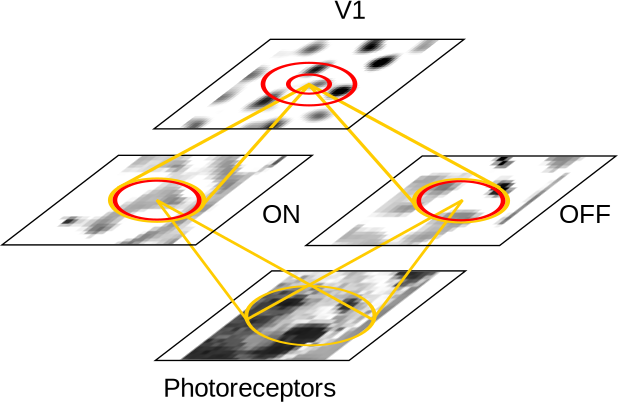
\includegraphics[scale=\schematicScale]{./figures/fig04.pdf}
}
\caption[General model architecture]{ \textbf{General model
    architecture.}  The four models discussed in this paper consist of
  two-dimensional arrays of computational units representing local
  groups of neurons at each visual processing stage. Connections to
  one unit in each sheet are shown with afferent connections in yellow
  and lateral connections in red. The V1 region shown here covers
  approximately 4mm$\times$4mm of ferret cortex, matching the cortical
  area represented by all the simulated orientation map plots in this
  paper. V1 units receive lateral excitatory (small circle) and
  lateral inhibitory (large circle) connections from nearby V1 units,
  leading to the `bubbles' of activity seen on the V1 sheet.
  V1 units receive afferent input from sheets
  representing the ON and OFF channels, representing the action of
  retinal ganglion cells and the lateral geniculate nucleus, which in
  turn receive input from the retinal photoreceptors. The
  difference-of-Gaussian afferent connections from the photoreceptors
  to the ON and OFF units form a local receptive field on the retina,
  and cause ON-center units to respond to light areas surrounded by
  dark, and OFF-center units to dark areas surrounded by light.
  Neighboring neurons in the ON and OFF sheets have different but
  overlapping receptive fields.  Input to the retinal photoreceptors
  can be any type of patterned image, such as the small natural image
  patch shown here. The GCL and GCAL models discussed later have
  additional lateral inhibitory connections within the ON and OFF
  sheets, but otherwise all four models discussed share identical
  initial weight profiles, spatial extents, and projection
  strengths.} \label{fig:modelarchitecture}

\end{figure}

The models are implemented in the Topographica simulator, freely
available at topographica.org. Topographica allows simulation
parameters to be specified in measurement units that are independent
of the level of detail used in any particular run of the
simulation. To achieve this, Topographica provides multiple spatial
coordinate systems, called sheet and matrix coordinates. Parameters
(such as sheet dimensions) are expressed in continuous-valued sheet
coordinates. In practice, of course, sheets are discretized using some
finite matrix of units. Each sheet has a density,
which specifies how many units (matrix elements) in the matrix
correspond to a unit length in sheet coordinates.  Each of these
simulations used a density of 98 neural units per sheet coordinate in
V1, and 24 units per sheet coordinate in the retinal photoreceptor and
ON/OFF sheets. Results are independent of the density used, except at
very low densities where discretization artifacts can become
prominent.

In all simulations shown, the area of the V1 sheet plotted and
analyzed has sheet-coordinate dimensions 1.0$\times$1.0, thus
consisting of 98$\times$98 neural units. The underlying simulated V1
area is actually 1.5$\times$1.5 (147$\times$147 neural units), which
is then cropped to 1.0$\times$1.0 for analysis and display, to
eliminate border effects due to partial
patterns of lateral connectivity for neurons
near the edge of the cortical sheet. The ON/OFF channels and photoreceptors are
similarly extended for simulation to 3.0$\times$3.0 and
3.75$\times$3.75 in sheet coordinates, respectively, to avoid having
any afferent receptive field cropped off, and to avoid edge effects in
the ON and OFF channels due to gain control connections when present.
In figure \ref{fig:modelarchitecture}, all sheets are shown at the
same size for visibility, but the actual area mapped topographically
between sheets was the central 1.5$\times$1.5 region of each sheet
that corresponds to V1.



\subsection*{Temporal properties}

As a simplification, we have ignored the detailed temporal properties
of the subcortical neural responses and of signal propagation along
the various types of connections. Instead, the model ON/OFF units have
a constant, sustained output, and all connections have a constant
delay, independent of the physical length of that connection.  One
training iteration in the model represents one visual fixation (for
natural images) or a snapshot of the relatively slowly changing
spatial pattern of spontaneous activity (for retinal waves).  I.e., an
iteration consists of a constant retinal activation, followed by
processing at the ON/OFF and cortical levels.

For one iteration, assume that input is drawn on the photoreceptors at
time $t$ and the connection delay is defined as $\delta t=0.05$. Then
at $t+0.05$ the ON/OFF cells compute their initial activation, at time
$t+0.10$ the ON/OFF cells incorporate lateral inhibition for gain
control (if present in this model), and at $t+0.15$ V1 begins
computing. At $t+0.20$ and every $0.05$ iterations until $t+1.0$, V1
continues to compute in a series of settling steps,
a fixed number sufficient to ensure that cortical
activity is no longer changing significantly (data not shown).
During this period, the retinal activity is assumed to be constant, to
reduce computational requirements.

\subsection*{Stimuli}

Images are presented to the model at each iteration by activating the
retinal photoreceptor units. The activation value $\Psi_{i}$ of
unit $i$ in the photoreceptor sheet ($P$) is given by the gray-scale
value in the chosen image at that point.

The images used here are either oriented and elongated two-dimensional
Gaussian patterns, disk-shaped patterns of noisy activation, or natural image
patches, which together cover a range of different input types so that
we can evaluate the robustness of map development. The center
coordinates and orientation of each Gaussian are chosen from a uniform
random distribution and cover an area of the photoreceptor sheet that
is a third wider and taller than V1, so that even V1 units near the
borders will see an approximately uniform distribution of each part of
the Gaussian blobs.  For Gaussian patterns the contrast is defined as
the percentage of the input range 0.0 to 1.0.

Noisy disk patterns create a circular region of activity with a radius
that is a substantial portion of the size of the photoreceptor sheet
in order to generate distinct edges; the activation is smoothed at the
edges of the disk with a Gaussian blur
\citep{bednar:neurocomputing04-or}.  Disk centers are chosen from a
uniform random distribution larger than the retinal photoreceptor
sheet size to allow for V1 units to see a uniform distribution of disk
areas.  Uniform zero-mean random noise is then added to the disk
pattern.

Natural image patterns are photoreceptor-sheet sized patches from
images of natural objects and landscapes, from a dataset by
\citet{Shouval1996}.  The pictures were taken at Lincoln Woods State
Park in Rhode Island, USA and scanned into a 256$\times$256 pixel
image. No corrections were used for the optical distortions of the
instruments and there was no pre-processing of the images. The dataset
used to approximate vertical goggle rearing shown
in figure \ref{fig:naturalsets} consists of the same
  set of image patches, but blurred by convolution
  with an anisotropic Gaussian kernel. The convolution kernel is a
  128$\times$128 matrix, consisting of a centered, vertical Gaussian
  pattern with an aspect ratio of $10$ ($\sigma_x=0.25$,
  $\sigma_y=0.025$ in unit sheet coordinates) and total weight of
  unity.

\subsection*{The ON/OFF sheets}

At each iteration, a new retinal input is presented and the activation
of each unit in each sheet is updated. Neurons in all sheets are
firing-rate point neurons, with a state characterized by an activation
level.  For all models, the activation level $\eta$ for a unit at
position $j$ in an ON/OFF sheet O at time $t+\delta t$ is defined as:

\begin{equation}
\eta_{j, O}(t+\delta t)=f\left(\frac{\gamma_{O}\sum_{i\in F_{j,P}}\Psi_{i}(t)\omega_{ij}}{k+\gamma_{S}\sum_{i\in F_{j,S}}\eta_{i, O}(t)\omega_{ij, S}}\right)
\label{eqn:lgnactivation}
\end{equation}

The constant $\gamma_{O}=14.0$ is an arbitrary multiplier for the
overall strength of connections from the photoreceptor sheet to the
ON/OFF sheets, chosen to give typical activations in the range 0.0 to
1.0, while $\gamma_{S}$ is the strength of the feed-forward
contrast-gain control. $\Psi_{i}$ is the activation of unit $i$ in the
two-dimensional array of neurons on the photoreceptor sheet from which
ON/OFF unit $j$ receives input (its afferent connection field
$F_{j,P}$) and $\eta_{i, O}(t)$ is the activation of other ON/OFF units on
the previous time step (received over the suppressive connection field
$F_{j,S}$). The activation function $f$ is a half-wave rectifying
function that ensures the activation of ON/OFF units is always positive.

In the L and AL models where contrast-gain control is not applied,
$k=1$ and $\gamma_{S}=0$, whereas in the GCL and GCAL models $k=0.11$
and $\gamma_{S}=0.6$.  The constant $k$ ensures that the output is
always well defined for weak inputs, and $\gamma_{S}$ is chosen to
re-scale activation values so that the numerical results are
comparable with and without gain control.

The weights $\omega_{ij}$ represent the fixed connection weights from
photoreceptor $i$ to the ON or OFF unit $j$ defined with a standard
difference-of-Gaussians kernel. The connection fields for ON units
have a positive center and negative surround, and vice versa for OFF
units. More precisely, the weight $\omega_{ij}$ from an ON-center cell
at location (0,0) in the ON sheet and a photoreceptor sheet in
location $(x,y)$ on the photoreceptor sheet is given by:
%%
\begin{equation}
\omega_{ij}=\frac{1}{Z_c}\exp{\left(-\frac{x^{2}+y^{2}}{2\sigma_{c}^{2}}\right)}-\frac{1}{Z_s}\exp\left(-\frac{x^{2}+y^{2}}{2\sigma_{s}^{2}}\right)
\label{eqn:DoG}
\end{equation}
%%
The width of the central Gaussian is defined by $\sigma_{c}=0.037$, and
$\sigma_{s}=0.15$ determines the width of the surround Gaussian, where
$Z_c$ and $Z_s$ denote the normalization constants that ensure the
center and surround weights each always sum to 1.0. The weights for an
OFF-center cell are the negative of the ON-center weights (i.e., surround
minus center). The center of the connection field of each ON/OFF unit
is mapped to the location in the photoreceptor sheet corresponding to the
location of that unit in sheet coordinates, making the projection
retinotopic.

The weights $\omega_{ij, S}$ in the denominator of equation
\ref{eqn:lgnactivation} specify the spatial profile of the
lateral inhibition received from other ON/OFF units when
contrast-gain control is active. The weights of these connections have
a fixed, circular Gaussian profile so that for a neuron located at
(0,0) in either the ON or OFF sheet:
%%
\begin{equation}
\omega_{ij,S}=\frac{1}{Z_S}\exp\left(-\frac{x^{2}+y^{2}}{2\sigma_{S}^{2}}\right)
\label{eqn:gauss}
\end{equation}
%%
where $(x, y)$ is the location of the presynaptic neuron,
$\sigma_{S}=0.125$ determines the width of the Gaussian, and $Z_S$ is
a normalizing constant that ensures that the total of all the lateral
inhibitory weights $\omega_{ij}$ to neuron $j$ sum to 1.0.  When
contrast-gain control is enabled, these recurrent lateral connections
are activated once per iteration, before activity is sent to the V1
sheet.

\subsection*{V1}

Each V1 neuron in each model receives connections from three different
connection types or `projections' ($p$), i.e., the afferent projection
from the ON/OFF sheets (both channels concatenated into one input
vector; $p=A$), the recurrent lateral excitatory projection ($p=E$),
and the recurrent lateral inhibitory projection ($p=I$) from other V1
neurons.

The contribution $C_{j,p}$ to the activation of unit $j$ from each
projection type ($p=A,E,I$) is calculated as:
%%
\begin{equation}
C_{j,p}(t+\delta t)=\sum_{i\in F_{j,p}}\eta_{i, p}(t)\omega_{ij,p}
\label{eqn:update}
\end{equation}
%%
where $\eta_{i, p}$ is the activation of unit $i$ taken from the set
of neurons in V1 to which unit $j$ is connected (its connection field
$F_j$) and $w_{ij,p}$ is the connection weight from unit $i$ in V1 to
unit $j$ in V1 for the projection $p$. Afferent activity ($p=A$)
remains constant after the first update from the retina, but the other
contributions change over 16 settling steps, depending on the activity
in V1.

The contributions from all three projections to V1 (afferent and
lateral) described above are combined using equation
\ref{eqn:activation1} to calculate the activation of a
neuron $j$ in V1 at time t:
%%
\begin{equation}
\eta_{j,V}(t)=f\left(\sum_{p}\gamma_{p}C_{jp}(t)\right)
\label{eqn:activation1}
\end{equation}

The projection strength scaling factors for each projection type $p$
are $\gamma_{A}=1.5$, $\gamma_{E}=1.7$, and $\gamma_{I}=-1.4$ for all
models, set to provide a balance between excitation and inhibition,
and between afferent and lateral influences, to provide robust
formation of activity bubbles that allows smooth maps to form. For
models L and GCL, $f$ is a
half-wave rectifying function that ensures positive activation
values. In the case where single-neuron automatic adaptation is
included (models AL and GCAL), $f$ has a variable threshold point
($\theta$) dependent on the average activity of the unit as described
in the next subsection, but in all cases the gain is fixed at unity.

Once all 16 settling steps are complete, the settled V1 activation
pattern is deemed to be the V1 response to the presented pattern. At
this point we use the V1 response to update the threshold point
($\theta$) of V1 neurons (using the adaptation process described
below) and to update the afferent and lateral inhibitory weights via
Hebbian learning. V1 activity is then reset to zero and a new pattern
is presented. Note that both adaptation and learning could instead be
performed at every settling step, but this would greatly decrease
computational efficiency.

\subsection*{Adaptation}

In order to set the threshold for activation, each neuron unit $j$ in V1
calculates a smoothed exponential average of its settled
  activity patterns ($\overline{\eta_{j}}$):
%%
\begin{equation}
\overline{\eta_{j}}(t)= (1-\beta)\eta_{j}(t) + \beta\overline{\eta_{j}}(t-1)
\label{eqn:averaging}
\end{equation}

The smoothing parameter ($\beta=0.991$) determines the degree of
smoothing in the calculation of the average. $\overline{\eta_{j}}$ is
initialized to the target average V1 unit activity ($\mu$), which for
all simulations is $\overline{\eta_{jA}}(0) = \mu= 0.024$. The
threshold is updated using:
%%
\begin{equation}
\label{eqn:thresholdupdate}%
\theta(t)= \theta(t-1) + \lambda(\overline{\eta_{j}}(t) -\mu)
\end{equation}
%%
where $\lambda=0.01$ is the homeostatic learning rate. The effect of
this scaling mechanism is to bring the average activity of each V1
unit closer to the specified target. If the activity in a V1 unit
moves away from the target during training, the threshold for
activation is thus automatically raised or lowered in order to bring
it closer to the target. Note that an alternative rule with only a
single smoothing parameter (rather than $\beta$ and $\lambda$) could
be formulated, but the rule as presented here makes it simple for the
modeler to set a desired target activity $\mu$.

\subsection*{Learning}

Initial connection field weights are isotropic 2D Gaussians for the
lateral excitatory projection and uniformly random within a Gaussian envelope
for afferent and lateral inhibitory projections. Specifically, for a
neuron located at (0,0):
%%
\begin{equation}
\omega_{ij}=\frac{1}{Z_p}u\exp\left(-\frac{x^{2}+y^{2}}{2\sigma_{p}^{2}}\right)
\label{eqn:gaussrandomweights}
\end{equation}
%%
where $(x, y)$ is the sheet-coordinate location of the presynaptic
neuron, $u=1$ for the lateral excitatory projection ($p=E$) and $u$ is
a scalar value drawn from a uniform random distribution for the
afferent and lateral inhibitory projections ($p=A,I$), $\sigma_{p}$
determines the width of the Gaussian in sheet coordinates
($ \sigma_{A}=0.27, \sigma_{E}=0.025, \sigma_{I}=0.075$), and $Z_p$ is
a constant normalizing term that
ensures that the total of all weights $\omega_{ij}$ to neuron $j$ in
projection $p$ is 1.0.  Weights for
each projection are only defined within a specific maximum circular
radius $r_p$ ($r_{A}=0.27, r_{E}=0.1, r_{I}=0.23$).

In the model, as images are presented to the photoreceptors, V1
afferent connection weights $\omega_{ij,A}$ from the ON/OFF sheets are
adjusted once per iteration (after V1 settling is completed) using a
simple Hebbian learning rule. This rule results in connections that
reflect correlations between the pre-synaptic ON/OFF unit activities
and the post-synaptic V1 response.  Hebbian connection weight
adjustment at each iteration is dependent on the pre-synaptic
activity, the post-synaptic response, and the Hebbian learning rate:
%%
\begin{equation}
\omega_{ij,p}(t)=\frac{\omega_{ij,p}(t-1)+\alpha\eta_{j}\eta_{i}}{\sum_{k}\left(\omega_{kj,p}(t-1)+\alpha\eta_{j}\eta_{k}\right)}
\label{eqn:hebb}
\end{equation}
%%
where for unit $j$, $\alpha$ is the Hebbian learning rate for the
afferent connection field $F_{j}$. Unless it is constrained, Hebbian
learning will lead to ever-increasing (and thus unstable) values of
the weights \citep{Rochester1956}. In all the models the weights are
constrained using divisive post-synaptic weight normalization
(equation \ref{eqn:hebb}), which is a simple and well understood
mechanism. Afferent connection weights from ON and OFF units are
normalized together in the model. We expect that a more
biologically motivated
homeostatic mechanism for normalization such as multiplicative
synaptic scaling \citep{Turrigiano1999,Turrigiano2004,Sullivan2006}
or a sliding threshold for plasticity \citep{Bienenstock1982}
would achieve similar results, but have not tested these.

The learning rates for the afferent projection, lateral excitatory
projection and lateral inhibitory projections are
$\alpha_{A}=0.1,\alpha_{E}=0.0$, and $\alpha_{I}=0.3$ respectively.
The density-specific value used in the equation above is then
calculated as $\alpha=\frac{\alpha_{A}}{\tau_{A}}$, where $\tau_{A}$
is the number of connections per connection field in the afferent
projection. In order to increase computational efficiency, lateral
excitatory connections do not learn during development in the
simulations presented here. The effect of lateral learning has been
explored in detail in previous similar models \citep{Miikkulainen2005},
and the maps generated by GCAL are visually
indistinguishable regardless of whether or not lateral excitatory
connections are plastic (data not shown).

\subsection*{Analysis of model maps}

Model orientation maps are calculated based on the vector average method
\citep{Miikkulainen2005,Blasdel1986}. Sine grating inputs that cover
the full range of parameter values (combinations of all orientations,
frequencies, and phases) are presented, and for each orientation, the
peak response of the neuron is recorded. The orientation preference is
calculated by constructing a vector for each orientation $\theta$
(between $0^{\circ}$ and $180^{\circ}$) with the peak response as the
length and $2\theta$ as its orientation. These vectors are summed and
the preferred orientation is calculated as half of the orientation of
the summed vector. The selectivity is given by the magnitude of the
summed vector. Average orientation selectivity values are the mean
value of orientation selectivity across all units in the map and are
normalized by dividing by the maximum average selectivity measured
across all simulations reported in this paper.

Orientation tuning curves are measured by presenting sine gratings
with 20 different orientations, each at 8 different phases and for a
range of contrasts. For each contrast, the responses of each neuron
unit are measured and the maximum response at each orientation over
all phases is recorded. The tuning curve is constructed from these
maximum responses.

To ensure consistent map measurement across all conditions,
orientation maps in figures \ref{fig:metric} to
\ref{fig:gaussian_GCAL} are measured before lateral interactions and
the V1 activation function take affect (i.e., on the afferent input
activity only). Maps for models with gain control change little if
these steps are included.  However, for models without gain control,
if activation thresholds and lateral interactions were simulated
during map measurement, maps would need to be measured at many
different contrasts, because orientation tuning in these models is not
contrast invariant, and therefore orientation selectivity is difficult
to determine.  Instead, we use the orientation selectivity of the
afferent connections as a measure of the map selectivity in all
cases. This simplification allows fair and consistent comparison of
selectivity values between the simulations of all four models.
Similarly, connection field plots show the weights of connections
between the ON sheet and V1 at different times during development.
These weights are used as an approximation to the receptive fields
that can be measured using a computationally intensive reverse
correlation process that takes into account the full connectivity,
which again must control for contrast in the models without gain
control. The true orientation selectivity of neurons in the full
recurrent network is reflected in the orientation tuning curves for
the GCAL model (as shown in figure \ref{fig:tuningcurves}).

\normalsize

\section*{Results}
In this section we present results from four closely related
developmental models of orientation map formation, all
sharing the architecture illustrated in figure
\ref{fig:modelarchitecture}.  As described in Materials and Methods,
each model is a network of single-compartment firing-rate units, each
receiving afferent and lateral connections that are modified by
Hebbian learning.  The models share the same four sheets 
of simulated neurons representing the pathway from the retina to
V1, with the same dimensions, connection radii, initial weights,
and all other parameter settings.

The robustness of each model will initially be analyzed across a wide
range of input contrasts for an artificial input pattern (randomly
positioned and oriented elongated two-dimensional Gaussians).  These
simple patterns help make our reasoning about how each mechanism
affects map development clear and intuitive and are sufficient for
evaluating each model's robustness to input contrast.  In turn,
contrast is used as a well-defined and easily characterized proxy for
a variety of changes in input patterns that could affect how much V1
is activated for a given input, and could thus affect stability and
robustness.  Once all four models have been evaluated with respect to
contrast for Gaussians, we will show that the results still hold (with
no changes in model parameters) for more complex changes in the input
images that are more difficult to characterize.

For each model, we evaluate the orientation selectivity, map stability,
and map quality, and relate the results to data from ferrets.
The first model is a simple laterally connected model of orientation
map development that we will refer to as model L. Model L retains the
essential features of previous models in this genre \citep{Sirosh1997,Burger1999,Burger2001,Miikkulainen2005}, while omitting biologically
unrealistic mechanisms like lateral radius shrinking that also reduce
stability, as well as eliminating arbitrary manual interventions like
threshold changes or learning rate changes over development.

Subsequent models build on L, adding single-neuron homeostatic threshold
adaptation (model AL), feed-forward gain control (model GCL), and
lastly both mechanisms together (model GCAL). Justification for each
mechanism is discussed as it is introduced, but the details of these
two mechanisms are described in the Materials and Methods section.
The results show that as well as reproducing stable development, the
final GCAL model is robust to extreme changes in the input statistics,
even during the process of development.


\subsection*{Model L: A simple model of map development}

Results from simulated development in the L model are shown in figure
\ref{fig:L_development}. Each V1 model neuron receives excitatory
connections from an already retinotopically aligned set of ON/OFF
neurons and excitatory and inhibitory connections from other V1
neurons (see figure \ref{fig:modelarchitecture}). At each iteration,
two elongated and oriented Gaussian patterns are presented on the
model retina.  The afferent and lateral connections lead to the
formation of isolated bubbles of activity in V1 in response to the input
pattern. Initially random afferent weights between the ON/OFF units
and V1 then adapt based on the pre and post-synaptic activity, via a
simple Hebbian learning rule with divisive normalization (equation
\ref{eqn:hebb}). Neurons in each bubble thus learn their
topographically corresponding input pattern, while neurons in other
bubbles learn different patterns.  Over the course of development
(20,000 iterations), nearly all receptive fields become orientation
selective and a topographic organization for orientation is formed (figure
\ref{fig:L_development}). This topographic organization arises because
throughout the development process nearby neurons are similarly
activated, and therefore develop similar orientation preferences. This
process has been well documented in previous models
\citep{Miikkulainen2005,Burger1999}.
%%
\begin{figure}
\centerline{
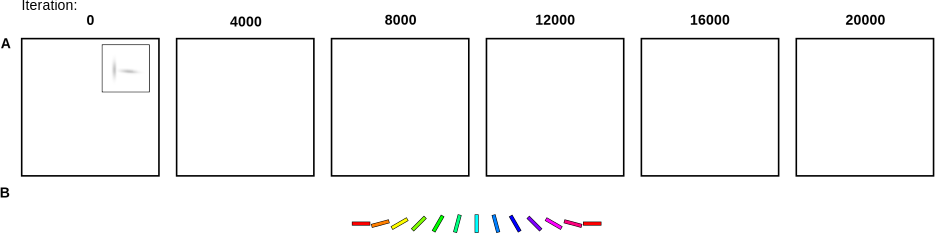
\includegraphics[scale=\LdevelopmentScale]{./figures/fig05.pdf}
}
\caption[]{\textbf{Model L develops maps but is not stable.}  
          (A) Model development at six different
          iteration time points for a single simulation.
          Self-organization was driven by two elongated Gaussian
          patterns at 25\% contrast per iteration, with an example
          inset into the plot for iteration 0.  Polar orientation maps
          from the beginning of development to the final map at
          iteration 20000 are shown. Each unit is color coded
          according to orientation preference, as shown by the color
          key. The brightness and saturation of the color indicates
          the strength of orientation tuning of the afferent
          connections, and each panel corresponds to approximately
          4mm$\times$4mm of visual cortex (a 1.0$\times$1.0 area in
          sheet coordinates).  (B) Afferent connections 
          from the ON sheet to V1 (CFs) are shown for an arbitrary set
          of V1 units thoughout development. Initially random
          connections are strengthened and weakened by Hebbian
          learning, forming orientation selective receptive fields,
          but the map patterns change significantly over time.
          These results, while an improvement
          over existing models that have additional, biologically
          implausible mechanisms for reducing stability to improve
          their final map organization, represent a baseline for the
          results of the later models (AL, GCL, and GCAL). The
          behaviour of L is analyzed further in figure
          \ref{fig:gaussian_L}, and the last map shown corresponds to
          figure \ref{fig:gaussian_L}E.}
  \label{fig:L_development}
\end{figure}

L is a greatly simplified model, explicitly designed to demonstrate
this process of self-organization using a minimal set of mechanisms.
The afferent input to V1 is a linear rectified function of the image
contrast (since the output of ON/OFF units is a linear function of the
overall input from the retinal photoreceptors), as shown in figure
\ref{fig:gaussian_L}A.  The activity of each LGN unit is the dot
product of the photoreceptor input and a normalised
difference-of-Gaussian ON- or OFF- receptive field, and the relation
between LGN activity and V1 afferent response is also linear. Unlike
the LGN units, a V1 unit will not respond until the sum of its input
activities exceeds a fixed minimum threshold $\theta$ (figure
\ref{fig:gaussian_L}B).
%%
\begin{figure}
\centerline{
\includegraphics[scale=\GaussianScale]{./figures/fig06.pdf}
}

\caption[]{\textbf{Model L: Basic model has relatively poor
    stability, map quality, and robustness to contrast.}
  (A-B) The transfer
  functions from photoreceptor activity to LGN activity and from LGN
  activity to V1 afferent response respectively. Both transfer
  functions have unit slope and V1 units have a fixed threshold of
  $\theta=0.2$. (C) The mean map stability (green), selectivity (red)
  and map quality (blue) as a function of contrast, across ten
  simulations with randomized input sequences. Shaded areas indicate
  $\pm$95\% confidence intervals.  For low-contrast inputs, neurons
  are not activated and thus no learning occurs (point D); at slightly
  higher contrasts neurons have higher stability and selectivity
  (point E), but at the highest contrasts (point F) neurons are very
  unstable.  Neurons have a relatively high selectivity and stability
  in a small range of contrasts for which the model has been tuned
  (contrasts 15-30\%).
  (D-F) Organization of Model L at the end of development
  (iteration 20,000) at 10\%, 25\%, and 100\% contrast, respectively.
  Polar orientation preference maps with estimated pinwheel
  positions, along with sample inputs (inset), and afferent
  connections (CFs) from the ON sheet to V1 neurons for an arbitrary
  selection of model neurons (evenly spaced along the vertical midline
  of the map). The corresponding two-dimensional Fourier transforms
  (FFTs) are shown, with 1D spectral power histogram (green), function
  fit (red) and estimated peak position (blue arrow). These values
  determine the value of the map metric, which is fairly poor even for
  the best L maps due to the large number of pinwheels identified.  On
  the right, the stability and selectivity are plotted as a function
  of simulation time for that contrast, showing the average across all
  ten random seeds with the $\pm$95\% confidence intervals. (D) For
  low contrast inputs (contrast 10\%) orientation
  maps do not develop, yielding nominally
  high stability values that are meaningless because the selectivity
  remains low.  (E) Maps are well ordered and development is somewhat
  stable, within the `tuned' range of contrasts (contrast 25\%, as
  shown in figure \ref{fig:L_development}). (F) Orientation maps for
  high contrast patterns (100\% contrast) are highly disorganized,
  with sharp boundaries between hypercolumns and a non--ring-shaped
  FFT. Afferent connections are highly orientation selective imprints
  of the elongated Gaussians presented to the photoreceptor sheet, and
  map development is highly unstable, indicated by an early rise in
  selectivity without a corresponding increase in stability.
  Note that the final value of each stability plot will always be 1.0;
  the final map compared with itself has a stability index of
  unity. Overall, although L develops maps, it fails to be robust to
  contrast, develops relatively poor quality maps, and is not very
  stable compared to the ferret data.}
\label{fig:gaussian_L}

\end{figure}

The robustness of this model to changes in input stimulus is evaluated
by the behaviour of the model as a function of input contrast, without
changing any other parameters. Although there are many other
dimensions over which these inputs could be varied (e.g., number of
Gaussian patterns, size of pattern, amount of noise), robustness to contrast is an
intuitive feature that can be easily evaluated and related to the
visual system.  The analysis of this simple model
is shown in figure \ref{fig:gaussian_L}C. For each contrast, the
average stability over development (measured at intervals of
1000 iterations), the average orientation
selectivity of afferent connections in the final map (iteration
20,000) and average map quality of the final map are computed by taking
the mean results of ten different random seeds controlling the pattern
of training inputs. These three
measures give a good indication of the stability, robustness, and
quality of map development for each input image contrast. A fixed set
of three contrasts has been chosen for illustration and analysis in all
four models: the low-contrast point (D), the medium-contrast point (E)
and the high-contrast point (F). The medium contrast level of 25\% is
also shown in figure \ref{fig:L_development} and was selected as the peak
of the map metric for the L model.

Figure \ref{fig:gaussian_L}C shows that low-contrast inputs to the L
model (15-20\% contrast) can result in higher stability but lower map
quality than shown in figure \ref{fig:L_development}.  At these low
contrasts, neurons become moderately selective and a small degree of
stability can be achieved because, as the receptive fields of the
model neurons form, connections that have been strengthened by Hebbian
learning continued to strengthen throughout development, rather than
being overwritten by the strengthening of a different set of
connections. Figure \ref{fig:metric}D illustrates that
the pinwheel densities at these contrasts are reliably distinguishable
from biological maps; average results from 33 simulations
of the L model at 15\% contrast are shown.

In this model, contrasts of 10\% and below (e.g.\ map \ref{fig:gaussian_L}D) lead to a
complete lack of map development. If the pre-synaptic ON/OFF activity
is not strong enough to consistently exceed the necessary fixed
threshold $\theta$ to activate V1 neurons, connections will not change
and receptive fields will not form. Such a developmental process is
thus completely stable at the cost of achieving any degree of
selectivity. Although this is a trivial property of the L model, the
ability of the early visual system to ensure that V1 is sufficiently
activated is an important consideration for understanding visual
development.

As input image contrast increases, both the stability of map
development and the overall level of map organization degrades
rapidly, resulting in maps such as the one shown in figure
\ref{fig:gaussian_L}F at high contrast.  The map organization of the
orientation map in F can be seen to be very poor, as reflected by
the non ring-shaped structure in the Fourier power
  spectrum. These observations hold across all ten randomized
simulation runs, as demonstrated by the low value of the $\pi$
pinwheel density metric for all high-contrast measurements (figure
\ref{fig:gaussian_L}C).

In general, the L model is \emph{not} robust to contrast.  Unlike the
experimental data shown in figure \ref{fig:ferret_stability}A, selectivity is
achieved rapidly but map stability over development is not
maintained. There are several key properties of this simple model that
make it a poor model of robust map development in animals.  First, the linearity
of activity in the LGN and V1 with respect to photoreceptor activity
ensures increases in contrast directly lead to corresponding increases
in activity in ON/OFF units as well as in V1. Second, the lateral interactions
in the model depend on the level of activation of V1 units and further
amplify activity in V1 as input image contrast increases. Third, as
the afferent weights in the model develop, receptive fields of V1
neurons become more orientation selective and therefore match the
patterns in the input more closely, further increasing the
postsynaptic responses of V1 neurons. These three properties ensure
that during development, when inputs are high contrast, both ON/OFF
and V1 activity will also be high.

With a fixed Hebbian learning rate, the consequence of simultaneously
elevated pre- and postsynaptic activity (from the high ON/OFF and V1 responses respectively) ensures that the amount of Hebbian learning is increased (see
equation \ref{eqn:hebb}).  Therefore, with high contrast input,
connections between ON/OFF and V1 cells are more likely to be
overwritten as differently oriented patterns are presented, leading to
continual reorganization of receptive fields and a corresponding loss
of stability and overall map quality.

Conversely, selectivity of receptive fields increases as contrast is
increased.  This is because, as contrast increases, connections begin
to strengthen and weaken on a faster timescale, eventually becoming
indicative of the most recent pattern on the retinal photoreceptors
(which in this case will be a highly selective, elongated Gaussian
pattern) rather than learning to represent longer-term correlations in
the afferent input.

This simple model, although capable of forming orientation-selective
receptive fields and smooth topographic organization for orientation
(given a particular set of parameters) is not robust even to small
changes in the input image contrast.  Since experimental results
indicate that map development is robust and stable over a timescale
relatively consistent between animals, and that the input activity
properties are likely to change during development (for example,
before and after eye opening), it is necessary for the visual system
to have some underlying mechanism that compensates for changes in the
type of driving input.

The following sections show how feed-forward gain control and
automatic adaptation of the neuronal activation thresholds can improve
the stability of orientation map development and robustness in
response to changes in the input image properties.  We then show how
inclusion of both these simple and biologically motivated mechanisms
results in the development of other emergent properties of V1 neurons,
such as contrast-invariant orientation tuning.

\subsection*{Model AL: Homeostatic adaptation regulates postsynaptic activity}

In the L model, the fixed activity threshold across all V1 units was
found to constrain robustness to contrast. For any positive threshold
value, there will be a range of low contrasts at which the input to V1
units is below threshold and no development occurs. At high contrasts,
the postsynaptic activity of the V1 units will be unbounded, resulting
in map instabilities due to rapid Hebbian learning constantly
reorganizing receptive fields across the map.

In biological V1, the firing rates of different cortical neurons cannot be
characterized by a single, linear (and therefore unbounded) function
of synaptic input. Unlike the linear model units with fixed threshold,
real neurons are thought to have intrinsic homeostatic plasticity,
whereby each neuron regulates the level of synaptic input required to
generate an action potential by changing the number and distribution
of its ion channels \citep{Davis2001,Daoudal2003,Schulz2006,Zhang2003,Grubb2010,Kuba2010}. Such mechanisms allow each neuron
to adapt its firing threshold in order to maintain a
suitable average activity as incoming synaptic drive varies over time.

In the AL model, a simple model of homeostatic adaptation is
introduced to the cortical sheet, allowing individual V1 units to
adjust their firing thresholds to establish a suitable average target
activity (equation \ref{eqn:thresholdupdate}). The response of the
ON/OFF units remains linear with respect to the photoreceptor activity
(shown by figure \ref{fig:gaussian_AL}A) but the relationship between
ON/OFF response and V1 afferent activity is now illustrated by figure
\ref{fig:gaussian_AL}B.
%%
\begin{figure}
\centerline{
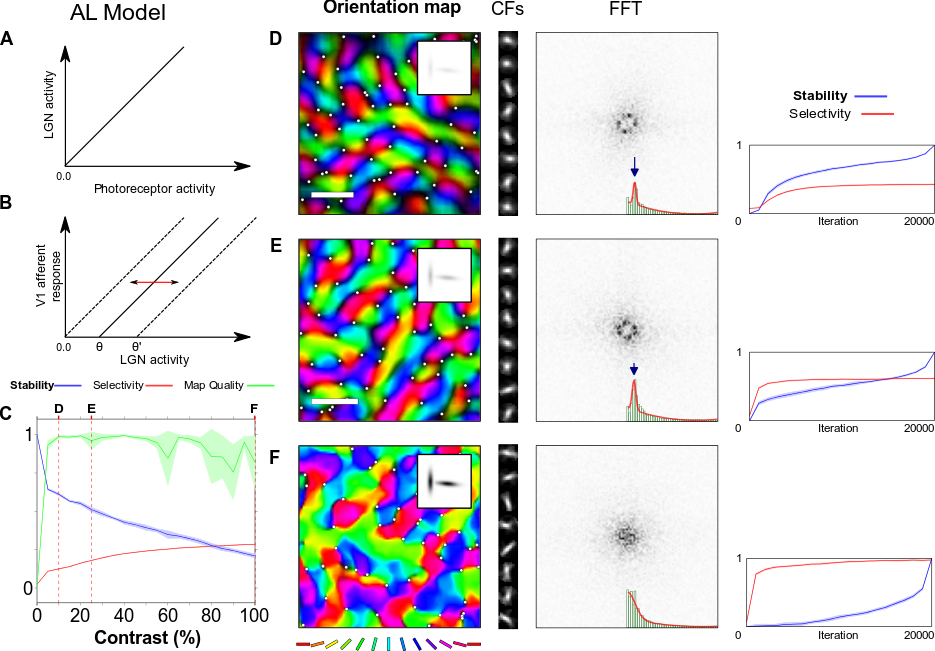
\includegraphics[scale=\GaussianScale]{./figures/fig07.pdf}
}

\caption[]{\textbf{Model AL: Adding homeostatic threshold adaptation
    improves selectivity, stability and map quality across all contrasts.} 
  (A) The transfer function from photoreceptor activity to LGN activity
  remains unchanged. (B) Each V1 unit now possesses an independent
  adaptive threshold $\theta$ that is automatically adjusted to
  maintain a fixed target activity. (C) Maps are more stable across
  contrast, with higher selectivities at high contrast than the L
  model. Map quality is relatively high throughout, with a drop at high
  contrasts. (D) The AL model can respond and self-organize at lower
  contrasts by lowering the adaptive threshold of V1 units. (E) AL
  self-organizes into higher-quality maps than L at identical
  contrasts, though stability has suffered compared to (D).  (F)
  Adaptation greatly improves the map quality relative to the L model
  at high contrasts. However, the map still suffers from sharp
  boundaries due to highly selective connection fields that are
  imprints of the elongated Gaussians presented to the photoreceptor
  layer, and the FFT becomes non--ring-shaped at high contrast.
  Stability is also very poor (with selectivity achieved long before
  stability), because the afferent weights continually reorganize at
  high contrasts.  Thus homeostatic adaptation offers significant
  benefits over the L model, but is not sufficiently robust or stable
  to account for the animal data.}
\label{fig:gaussian_AL}
\end{figure}

The quality and robustness of AL across input contrast is greatly
improved by the introduction of adaptive thresholds, suggesting that
intrinsic homeostatic adaptation plays an important role in robust map
development (figure \ref{fig:gaussian_AL}C). With adaptation, maps
have more realistic pinwheel densities and stability drops off more
slowly at high contrasts. At the low-contrast point shown in figure
\ref{fig:gaussian_AL}D, self-organization is able to proceed as the
adaptive thresholds fall, ensuring activity in the V1 sheet and
compensating for the lower input levels.

At the mid-contrast point shown in \ref{fig:gaussian_AL}E,
selectivity and stability are higher and the maps are better organised
than in the L model. This is demonstrated by the higher map metric,
which reflects the greater spacing between pinwheels in the orientation map and the
increasingly ring-shaped Fourier power spectrum.

At high contrasts, selectivity continues to increase but map quality
and stability start to fall. The orientation map shown in figure
\ref{fig:gaussian_AL}F is highly selective everywhere, including
around the identified pinwheel locations. The result is a map with
sharp boundaries between regions of different orientation preference
instead of smooth transitions.  The variance in
pinwheel density increases as the ring structure in the FFT degrades,
due to the hypercolumn distance becoming poorly defined in Fourier
space. The high selectivity is also evident in the highly elongated
weight profiles of the afferent connectivity from the ON/OFF sheets to
the V1 units.

The failure of the AL model at high contrast is due to the same
fundamental problem identified in the L model: rapid Hebbian learning
in the afferent connectivity from the LGN to V1. Although the
postsynaptic activity is now homeostatically regulated, which keeps
the intracortical circuitry working in a well-defined range, the
presynaptic activity in the ON and OFF layers remains unbounded.  The
result is an effectively very high afferent learning rate, causing
recent inputs to be memorized rather than being incorporated smoothly
into the map, and destroying stability.  Moderating the postsynaptic
activity can only partially address this imbalance, so long as the
activity in the presynaptic ON and OFF sheets remains unbounded.

\subsection*{Model GCL: Gain control compensates for differences in input strength}

Rather than compensating for high presynaptic activity by regulating
postsynaptic excitability, an alternative and perhaps more direct
approach would be to limit the range of possible activity levels
reaching V1. This change would ensure that learning in the afferent
connections between the ON/OFF sheets and V1 cannot be disrupted by
high presynaptic activity.

Contrast-gain control, also known as normalization, is a
well-documented phenomenon whereby neurons have a nonlinear response
to input strength, compressing a wide range of inputs into a smaller
range of responses \citep{bonin:jn05}.  There is a wealth of
experimental evidence supporting the idea that contrast-gain control
first arises early in the visual pathway
(e.g.\ \citealp{Shapley1978,Baccus2002,Derrington1984,Sclar1987,Alitto2004,Truchard2000}).
A wide variety of candidate mechanisms have been proposed
(\citealp{Carandini2002,Geisler1997,Finn2007,Anderson2000}; see
\citealp{Heegerreview} for review).

In the GCL model, contrast-gain control is implemented using divisive
inhibitory lateral connections between model ON/OFF neurons, providing
an `extra-classical' supressive surround
\citep{Felisberti1999,bonin:jn05,Alitto2008}. We would
expect to obtain similar results using the other mechanisms that have
been proposed, but have not tested them.
%%
The addition of gain control to the L model ensures that the afferent
input to V1 is no longer a linear function of the input image
contrast, as shown in figure \ref{fig:gaussian_GCL}A. Instead, the
afferent input to V1 saturates with increasing contrast.
%%
\begin{figure}
\centerline{
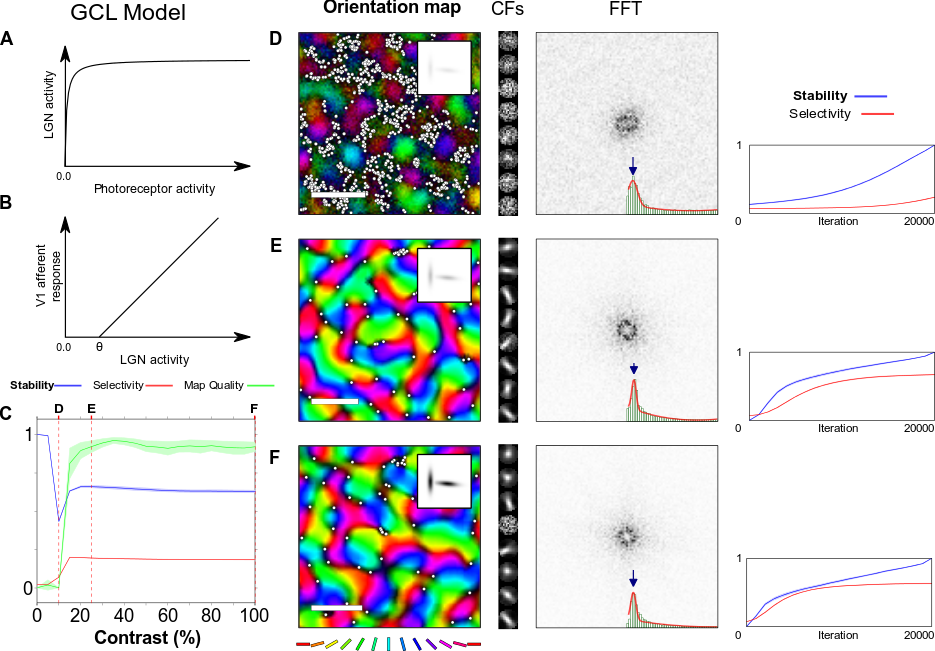
\includegraphics[scale=\GaussianScale]{./figures/fig08.pdf}
}
\caption[]{\textbf{Model GCL: Adding contrast-gain control
    independently improves stability and map quality.}
  (A) Contrast-gain control in the ON/OFF sheets results in a
  non-linear transfer function, compressing unbounded photoreceptor
  inputs into a bounded range of LGN activities. (B) V1 units share
  the same fixed threshold as those in the L model. (C) Map quality is
  improved across all contrasts and map stability no longer degrades
  as contrast increases. Selectivity remains both high and stable with
  increasing contrast. (D) At the low contrast point, GCAL can just begin
  to self-organize as contrast-gain control boosts enough of the
  afferent signal over the fixed V1 threshold for some Hebbian
  learning to occur. (E) GCL self-organizes into higher quality maps
  than L at the same 25\% contrast level. Unlike the AL model, some
  small areas of the map fail to self-organize properly, resulting in
  regions of low selectivity and clusters of pinwheels. (F) For high
  (100\%) contrast inputs, map quality remains consistently high,
  connection fields remain well-formed, the map remains smooth and the
  FFT is appropriately ring-shaped. However, small areas of the map
  fail to self-organize or develop selectivity, as shown by the noisy
  connection field.  Overall, gain control supports robust and stable
  map development across contrasts, but some neurons are left behind
  as the others develop, and cannot reach threshold, leading to
  unevenly organized maps.}
\label{fig:gaussian_GCL}
\end{figure}

Figure \ref{fig:gaussian_GCL}C shows that gain control in the ON/OFF
sheets is sufficient to greatly increase the robustness and stability
of the orientation map development process. By compensating for
differences in the presynaptic input to V1, stability is greatly
improved, with high map quality across most contrasts. Stability no
longer degrades at high contrast, selectivity remains stable even at
high contrast, and map quality remains consistently high.

At the low-contrast point shown in figure \ref{fig:gaussian_GCL}D,
contrast-gain control has enabled some self-organization, boosting the
weak input signal over the firing threshold in the cortical layer. The
orientation map is not as well organized as the corresponding AL map
(\ref{fig:gaussian_AL}D), but this result does demonstrate that this
contrast-gain control mechanism amplifies weak afferent signals for
low-contrast inputs.

At the medium contrast level shown in figure \ref{fig:gaussian_GCL}E,
the orientation map is comparable to the equivalent AL map. One common
type of artifact observed in GCL are the pinwheel clusters found in
low-selectivity regions, which do not appear in maps that have adaptive
thresholds in the cortical layer (figure \ref{fig:gaussian_AL}). These
pinwheel clusters persist even in the high-contrast regime shown in
figure \ref{fig:gaussian_GCL}F.

The origin of these artifacts is illustrated by the afferent weight
pattern shown in figure \ref{fig:gaussian_GCL}F (fourth pattern
down). This set of weights is noisy and has failed to self-organize,
indicating areas of the map lagging in their development. These areas
of poor organization arise when neighbouring cortical regions develop
orientation selectivity slightly more quickly, increasing the postsynaptic
activity of these surrounding regions. This increase in the activity
of neighbouring units increases the strength of the suppressive
lateral interactions, further suppressing the development of the
region already lagging in self-organization. This positive-feedback
loop ensures that some areas of the map fail to develop properly.
Thus although GCL is a clear improvement over both L and AL, it does
not robustly organize into biological maps that include all of the
simulated neurons.

\subsection*{Model GCAL: Adaptation compensates for differences in V1 activation}

Homeostatic adaptation and contrast-gain control independently
improved map quality, selectivity and robustness, but both mechanisms
have been found to have specific shortcomings. The final GCAL model combines
the ON/OFF contrast-gain control mechanism from GCL (illustrated in figure
\ref{fig:gaussian_GCAL}A) with the adaptive threshold from AL
in the cortical layer (figure \ref{fig:gaussian_GCAL}B).

\begin{figure}
\centerline{
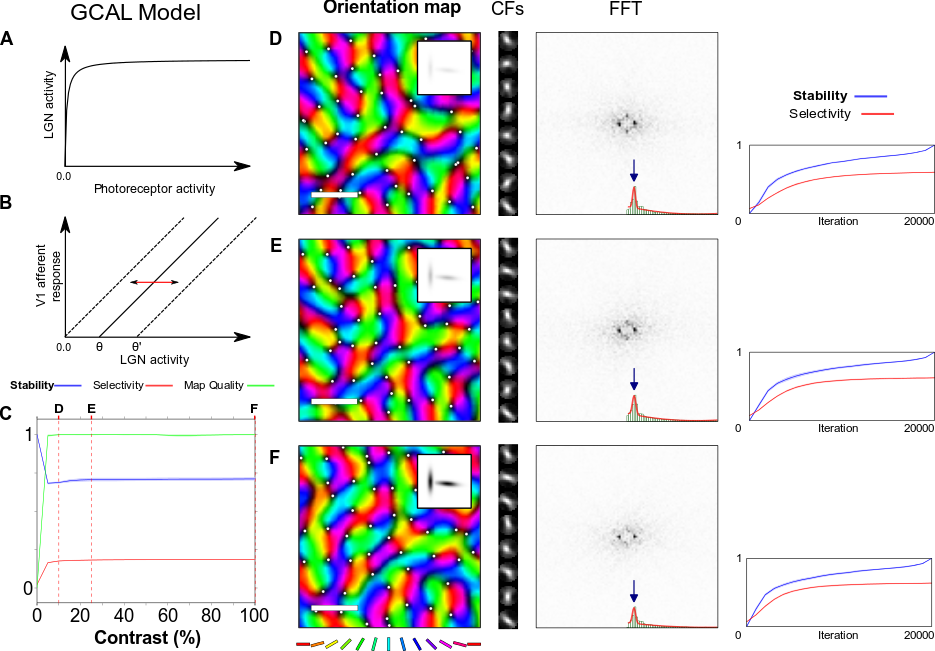
\includegraphics[scale=\GaussianScale]{./figures/fig09.pdf}
}

\caption[]{\textbf{Model GCAL: Combining homeostatic
    adaptation with gain control yields high-quality, selective,
    stable maps at all contrasts.} (A) The contrast-gain
  control mechanism introduced in GCL is retained. (B) V1 units now
  have the same adaptive threshold ($\theta$) as in the AL model.  (C)
  Map quality metric indicates that all GCAL maps have very close to $\pi$
  pinwheel density for all simulated orientation maps (also see Figure
  \ref{fig:metric}D), with high stability and selectivity across all
  contrasts. (D-F) Maps are properly self-organized at all contrasts,
  with ring-shaped FFTs. At high contrast, GCAL remains smooth and
  does not suffer from low-selectivity pinwheel clusters, due to the
  introduction of the homeostatic threshold. Stability increases
  alongside selectivity, indicating highly stable map development. The
  GCAL model robustly generates high selectivity, highly stable,
  high quality maps.}
\label{fig:gaussian_GCAL}

\end{figure}

Analysis of this model in figure \ref{fig:gaussian_GCAL}C
demonstrates that the combination of these two mechanisms results in a
model that is extremely robust to contrast, while organizing much more
smoothly and consistently at any contrast than the other models. All
maps at all visible contrasts achieve $\pi$ pinwheel density, as shown
by the map metric value.  As an illustration, the data for $40$ GCAL
simulations at 100\% contrast has been replotted in figure
\ref{fig:metric}D, where the cluster of red circles for
GCAL clearly fits into the range of pinwheel
density values seen in ferret maps. All FFT plots are ring-shaped and comparable to the
biological maps, and none of the maps suffer from the artifacts identified
in the AL and GCL models. Selectivity and map stability are achieved
rapidly once sufficient contrast is available, and remain constant
across all contrasts.

The maps at the low-, medium-, and high-contrast points are
qualitatively indistinguishable; all afferent weights develop properly
without becoming over-selective at the expense of map
quality. Combining gain-control and homeostatic adaptation achieves a
tradeoff between selectivity and map quality that results in highly
realistic orientation preference and selectivity maps that are
extremely robust to variations in contrast.

Evidently, homeostatic adaptation complements gain control by adjusting
the postsynaptic target activity of each V1 unit, ensuring the
long-term smooth development across the map over many visual inputs
and thus preventing any particular region of the map from being
under-activated and thus lagging behind in the self-organization
process. Homeostasis helps ensure consistent map development in spite
of fluctuations in the input statistics across multiple presentations,
by retaining a weighted history of previous activation.

Contrast-gain control in turn complements homeostatic adaptation by
compressing the dynamic range of each individual input, regulating the
presynaptic input between the ON/OFF sheets and the cortical layer and
ensuring the rate of Hebbian learning in the afferent connections
matches the rate of development of lateral cortical connectivity. Even
if the long-term average pre-synaptic activity in the ON/OFF sheets is
appropriate for normal Hebbian learning in the afferent connections,
the high dynamic range within a single visual input would continue to
disrupt the afferent connectivity on a timescales too rapid for the
homeostatic threshold to compensate. Contrast-gain control assists the
action of homeostatic adaptation over long timescales, normalizing the
dynamic range of activity of individual presentations and allowing the
activity threshold to respond to long-term trends in the input and not
to the transient variance within individual presentations.

These two mechanisms perform two different operations on different
timescales that independently increase the robustness of development to
input contrast. Together these two operations complement each others'
operation to adjust the average activity and dynamic range of the pre-
and postsynaptic neural activity to ensure robust map development
progresses smoothly and regularly on both long and short timescales.

\subsection*{Stable and robust development using realistic inputs in the GCAL model}

The previous sections looked only at robustness to image contrast, but
biological maps appear to be robust against not only the strength, but
also the frequency and type of patterns, with similar maps developing
with and without eyes open and with and without dark rearing.  We now
 examine how the GCAL model previously tested with the
abstract Gaussian input patterns can be used for other types of input
patterns, without changing any of the model parameters.

When an animal opens its eyes, the driving input to the LGN and V1
changes from spontaneously generated patterns to natural visual input
\citep{Beckmann1982,Tavazoie2000,Cragg1975,Huberman2006,Hooks2006}.
As described above, despite this change, orientation maps measured
at eye opening retain their orientation preferences, and therefore
mature into a final adult map that is similar to the map measured
at eye opening.  We can model pre--eye-opening development in the
GCAL model using input image patterns that resemble intrinsically
generated activity (loosely modeled after retinal waves
\citep{Wong1999}, and represented as noisy disk-shaped patterns
randomly placed on the retinal photoreceptors at each iteration
\citep{bednar:neurocomputing04-or}).  After eye opening, development can be modeled
using retinal inputs extracted from a dataset of natural images, from
\citet{Shouval1996}.

Figure \ref{fig:noisytonatural} shows results from the GCAL model,
which includes both gain control in the ON/OFF channels and
homeostatic adaptation, compared with experimental results from
chronic optical imaging in ferret.  In the model, when the input type
changes from noisy disks to natural images (at iteration 6000), there
is no decrease in the map orientation stability index (figure
\ref{fig:noisytonatural}E), even though selectivity continues to
increase. The initial map structure generated before model `eye
opening' is maintained after eye opening, despite the change in the
nature of the driving activity.  Note that no model parameters have
been changed from the previous simulations with Gaussian input
stimuli; the model is robust even to extreme changes in the input
images without the need for any compensatory changes in parameters.

It would not be possible to use these more realistic
inputs in the L or AL models without a significant retuning of the
parameters. Without contrast-gain control, individual image-patch
presentations with high contrast will disrupt the afferent
connectivity from the LGN to the V1 sheets, as in figures
\ref{fig:gaussian_L}F and \ref{fig:gaussian_AL}F.  The
GCL model is more robust to contrast changes, yet as shown in figure
\ref{fig:gaussian_GCL}F, development of individual neurons is not
robust, and thus only GCAL allows all neurons to develop robustly
across a wide range of inputs.

%%
\begin{figure}
\centerline{
\includegraphics[scale=\NoisytoNaturalScale]{./figures/fig10.pdf}
}
\caption[Stable map development before and after eye opening]
        {\textbf{Stable map development before and after eye opening.}
          (A) Polar orientation maps recorded using chronic optical
          imaging at different ages in one ferret (figure
          \ref{fig:ferret_stability}A, ferret 1-3-3630, reprinted from
          \citet{Chapman1996}). (B) Simulated GCAL polar orientation maps.
          Noisy disk patterns drive the map development until 6000
          iterations, after which natural images are presented to the
          model retina.  (A,B) Both the ferret and model map have a
          ring-shaped FFT (inset in the final map plot of each).  (C)
          Afferent connections from the ON sheet to V1 are shown for
          an arbitrary set of model V1 units thoughout development, to
          illustrate how neurons become more selective over time.
          (D) Orientation stability indices (SI, equation
          \ref{eqn:similarityindex}) across development for the ferret
          from (A), replotted from figure \ref{fig:chapman}B for
          comparison.  (E) SI for the simulation shown in (B).
          As selectivity develops in both the ferret and GCAL, the map
          smoothly increases in stability, indicating a highly stable
          process of development.  Stability can also be seen by
          tracking individual features of the orientation map across
          time, again for the ferret and for GCAL.  These results show
          that the mechanisms in GCAL are sufficient to account for
          the observed levels of stability in ferret map development.
}
\label{fig:noisytonatural}
\end{figure}

The stability of ferret map development is measured in figure
\ref{fig:chapman}A,B and \ref{fig:noisytonatural}D.  We cannot
directly compare iterations in the model with days in the experimental
data, because the precise date of any initial starting point in the
ferret is unclear. However, we can qualitatively compare the overall
pattern of stable development for the experiment over the first 10000
iterations, which covers the period when selectivity and stability
rise before saturating in the model. In all the measured experimental
cases, selectivity values increase in conjunction with stability to
their maximum values over the course of development, which is also
true of the simulated data. In some ferrets in which the eyes are
surgically opened before the time of natural eye opening, very faint
maps were already seen and were already more similar to the final map
than to the control condition. Similarly, model maps which have begun
to develop before eye opening are similar to the final map (figure
\ref{fig:noisytonatural}E). These results are similar to the average
development for all eight ferrets shown in figure \ref{fig:chapman}B
and are consistent with binocular deprivation experiments in cat
\citep{Crair1998}.

Of course, map stability could be achieved trivially by decreasing the
ability of neurons to adapt once an orientation map is initially
formed before eye opening (for example, by forcibly decreasing the
Hebbian learning rate, as in many models). However, as shown in
various experimental studies, maps continue to adapt and mature after
eye opening, and ultimately come to reflect some of the underlying
statistics of the natural visual input.
%%
For example, figure \ref{fig:naturalsets}A shows experimentally
measured biological maps with and without continuous
exposure to one particular orientation, using a goggle-rearing
oriented-blurring paradigm (reprinted
from \citealp{Tanaka2009}). These experimental results suggest that when
exposed to one particular orientation after eye opening, orientation
maps in V1 reorganize by expanding the domains in the map that
maximally respond to the goggle-reared orientation, while reducing the areas
responding to the unexposed orientations. We can test this property in
the GCAL model by using post--eye-opening image data sets with
different orientation statistics.  Such results are
illustrated in figure \ref{fig:naturalsets}D, where the map is
developed using the same set of natural image
  patches used in figure \ref{fig:noisytonatural} after they have each
  been convolved with a vertically elongated Gaussian kernel,
  approximating the anisotropy introduced by goggle rearing. The
resulting orientation map also contains a much higher proportion of
vertical-preferring neurons. The differences between the model map
before and after eye opening, and as the map develops, show that as
in the experimental data, domains of the model V1 preferring the
predominant orientation have expanded as the map has matured. GCAL is
therefore robust and stable, but also able to adapt to changes in the
input statistics.
%%
\begin{figure}
\centerline{
\includegraphics[scale=\GRScale]{./figures/fig11.pdf}
}
\caption[Experimental and model orientation maps developed in
  orientation restricted environments] {\textbf{Experimental and GCAL
    model orientation maps developed in orientation-biased
    environments.}  (A) Orientation map measured in a normally reared
  kitten at postnatal day 84 and orientation
  histogram.  The color and brightness indicate the
    preferred orientation and the orientation magnitude,
    respectively. The color code for preferred orientations is shown
    to the side. The scale bars indicate 2 mm. (B) Orientation map
  measured in a kitten at postnatal day 42 after
  13 days of goggle rearing with
  vertical lines. Orientation histogram now shows
  a strong bias towards vertical orientations. Reprinted from
  \citet{Tanaka2009}. (C) Orientation preference
  maps during development from a GCAL simulation driven by noisy disk
  patterns until 6000 iterations, after which natural images
  that have been anisotropically blurred
    vertically are presented to the model retinal photoreceptors.
  (D) Histograms show an expansion of yellow
  (vertically preferring) regions in the orientation after eye
  opening, reflecting the statistics of the natural image input and
  reproducing the results observed in biological map development.}
    \label{fig:naturalsets}

\end{figure}

Finally, because the mechanisms added to make GCAL were not arbitrary,
but were chosen based on a wide range of well-established
experimental work, it is possible to make specific links between the
behavior of GCAL's neurons and experimental data.  For example,
contrast-gain control mechanisms have been proposed to be involved in
contrast-invariant tuning, whereby the tuning curves for V1 neurons
retain the same width across contrasts \citep{Sclar1982,Skottun1987}.
Figure \ref{fig:tuningcurves} shows that GCAL's self-organized
orientation-selective neurons have achieved robust contrast-invariant
tuning.  This property arises in the model because the
contrast-gain control in the ON/OFF channels increases the responses
to low-contrast relative
to high-contrast stimuli.  The recurrent lateral interactions in V1
then ensure that differences in the responses to preferred and
non-preferred orientations are amplified \citep{antolik:phd10}. Responses to non-preferred
orientations will therefore always be smaller than to preferred
orientations. Similar methods of achieving contrast-invariant
orientation tuning have been described in previous non-developmental
models \citep{Geisler1997,Anderson2000,Carandini2002,Finn2007}, but
to our knowledge GCAL is the first model to show how
contrast-invariant tuning using this method can emerge robustly over
development for a full map of V1 neurons.
%%
\begin{figure}
\centerline{
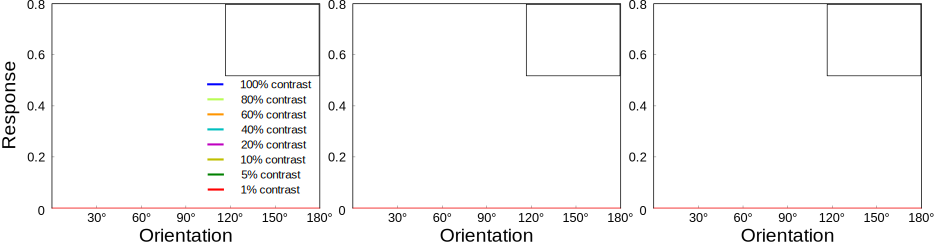
\includegraphics[scale=\ORTuningScale]{./figures/fig12.pdf}
}
\caption[Contrast invariant orientation tuning curves]
        {\textbf{GCAL model: Contrast-invariant orientation tuning.}
          Example orientation tuning curves for 3 representative model
          neurons, measured at the indicated contrasts. Orientation
          tuning width remains constant despite
          changes in contrast (except for small deviations at the
          lowest contrasts) as confirmed by the normalized tuning
          curves (inset).}
    \label{fig:tuningcurves}
\end{figure}

\section{Discussion}

We have shown that the integration of a small number of simple, well
known, biologically realistic mechanisms is sufficient to reproduce
stable and robust map development. Contrast-gain control in the early
visual pathway and homeostatic maintainance of activity levels have
the effect of regulating both the pre-synaptic activity and
post-synaptic activity of V1 neurons. This regulation can ensure that
throughout development, activity levels, and therefore the rate of
Hebbian learning, remain stable.  In this way, receptive fields of
individual neurons can approach a final organized structure without
being overwritten many times, thus achieving the stability and
robustness observed in experimental studies. These mechanisms also
potentially underlie contrast-invariant orientation tuning of
single neurons.

 Other activity-dependent models such as the elastic
  net have previously demonstrated stable development for orientation
  and for ocular dominance under certain conditions
  \cite{Wolfgang2011,Wolfgang2011PNAS}. However, these models are
  formulated at a more abstract level not suitable for identifying
  important mechanisms like homeostasis and gain control.  In
  particular, they do not simulate responses to individual input
  patterns such as natural images or retinal waves, and thus cannot
  address robustness with respect to changes in the input pattern
  types.

In the real biological system, the differences between input types may
be more (or less) extreme than those presented here, leading to two
possibilities.  Firstly, if the differences in the types of inputs that
drive the real visual system are more extreme, further adaptation
mechanisms may be required. For instance, if the density of edges in
visual scenes varies dramatically across different rearing
environments (e.g., between desert and jungle environments), it may be
necessary for the adaptation mechanism to take both pre and
post-synaptic activity into account together within each cell. We have implemented such
a mechanism in our modeling, but found that it was not necessary to
handle the range of input types considered here, while being less
obvious how to implement locally in V1 or LGN neurons. Alternatively, if
real input differences are less extreme, the mechanisms introduced
here may not both be required, although this is an unlikely
possibility given that there is substantial experimental evidence for
both of the simple mechanisms involved. The observation that these
mechanisms are also consistent with many other single-neuron
properties, such as contrast-invariant orientation selectivity and
automatic maintainance of average activity, suggests that the visual
system has achieved many different properties using similar underlying
mechanisms.

The ability of neurons to learn and adapt requires changes in synaptic
connectivity, yet it is also essential that neurons are neither
excessively active or silenced. Both excessive activity and silence
would lead to a loss of information at each level of the neural
pathway \citep{Turrigiano2004}, and so homeostatic adaptation not only
contributes to stable and robust map development but also helps to
maintain the transfer of visual information. More complex homeostatic
mechanisms may also stabilize map development, for example, by
regulating the distribution of activity rather than just the target
average value \citep{Triesch2005} or by operating on the synaptic
weights directly via a process such as synaptic scaling
\citep{Worgotter2011}. In any case, the idea that neurons use some
measure of their average activity over time in order to trigger
homeostasis and regulate their responses is widely accepted, and the
specific simple homeostatic mechanism used in GCAL is sufficient to
demonstrate how such regulation improves stability and robustness.

In the visual pathway, it is possible that both homeostatic adaptation
and contrast-gain control are present at every stage of processing. In
the GCAL model, we have chosen to apply the explicit contrast-gain
control mechanism only to the ON/OFF sheets and homeostatic adaptation
only to the V1 units. It would have been possible to add both of these
mechanisms to all the stages of the model, but this would have made
the effect of each mechanism harder to analyse and interpret, and we
do not believe such a change would affect our results
significantly.

GCAL depends heavily on lateral interactions.  Lateral interactions in
V1 arise because of lateral recurrent connections between neurons in
V1 (primarily in layer 2/3; \citealp{Gilbert1990,Bosking1997}). In
other simple self-organizing map algorithms, these specific lateral
interactions are replaced by a more convenient and computationally
efficient but highly abstract mechanism. For example, in the
Self-Organizing Map model
(\citealt{Obermayer1990,kohonen:original,farley:jn07}; SOM), the
algorithm finds the maximally active neuron in the cortex based on the
distance between the input pattern and each neuron's set of afferent
weights.  Afferent weights are then adapted only in a specified
circular (Gaussian) neighborhood around the maximally active
unit. There are therefore no specific lateral interaction strengths in
the SOM algorithm, weight changes depend only on the position of the
maximally active unit, and the cortical activity does not depend on
the contrast of the input stimulus. As shown in this study, we believe
that it is important to include specific lateral interaction strengths
in mechanistic models of V1 in order to understand the constraints on
the real system.

Although lateral interactions are important for the operation of the
GCAL model, the architecture is deliberately simplified and does not
reflect the detailed anatomy of cortical connectivity. In animals,
lateral interactions involve a complex circuit based on long-range
excitation and disynaptic inhibition, with different effects at
different contrasts \citep{Hirsch1991,Weliky1995}.  A model related
to GCAL demonstrates how this more elaborate circuit could give
similar results \citep{law:phd09}, but requires many more parameters
and more complicated analysis methods.  Similarly, a related model
shows how simulating multiple V1 laminae can explain both simple and
complex cells in V1, allowing neurons with random phase preferences to
develop in the simple cells and realistic orientation maps in the
complex cells \citep{antolik:fcn11}.  These other models improve on the
realism of the GCAL model, but because of their greater complexity and
the larger associated parameter spaces, they are more difficult to
analyze and understand, and so GCAL is more useful for studying
phenomena that do not require those additional circuit elements.

Apart from the lateral connectivity, another feature of the SOM and
other algorithms that is not shared by the GCAL model is that each SOM
V1 neuron begins with initial connections to the whole of the
retina. This starting point requires that both retinotopic and
orientation-selective receptive fields develop simultaneously.
Achieving smooth development of both these features in a computational
model requires several global ad-hoc mechanisms. For example, the
processes of lateral neighborhood decrease and learning rate decrease in
the SOM algorithm help ensure that self-organization does not fall
into a local minimum where the mapping is not retinotopic (i.e., they
provide an `annealing' of the map).  These ad-hoc mechanisms
themselves result in model orientation map instability, such as a
decrease in the size of orientation domains and a large reorganization
of the map over time.  However, real V1 maps are arguably formed
sequentially, with a coarse retinotopic map already in place before
the orientation map (reviewed in \citealt{Huberman2008}). In the model
algorithm presented here, there is an initial coarse retinotopic map
in V1, which avoids the need for global ad-hoc mechanisms to achieve
smooth map development.

The removal of ad-hoc mechanisms and addition of mechanisms explicitly
regulating activity levels makes GCAL easier to understand with
numerical simulations (as we have done here), and we expect the same
fundamental theoretical principles of operation to apply
to GCAL as for other self-organizing map models
\citep{vondermalsburg:selforg,kohonen:original}.  These properties
have been analyzed extensively in previous work  with
these related models.  In particular, GCAL
achieves good coverage and continuity in its representation of the
input feature space \citep{swindale:natneuro00} by forming sparse,
decorrelated activity bubbles in response to each input, just as in
LISSOM \citep{Miikkulainen2005}.  This process has been shown to fold a
high-dimensional feature space onto a two-dimensional surface, as a
discretized approximation of the principal surfaces of the input
\citep{ritter:neural}, and is a form of dimensionality reduction
\citep{durbin:dimension}.  We argue that GCAL should be seen as a
mechanistic implementation of the well-established principles of
self-organization, allowing them to proceed robustly for realistic
inputs of variable strengths and types.

Apart from the specific models introduced, we showed how pinwheel
density can be used to assess the quality of simulated orientation
maps.  Of course, pinwheel density is just one of many factors that
could be measured and compared between maps, but we argue that it is
a useful metric for several reasons.  First, there is a unique,
cross-species reference value, which allows objective decisions about
map quality.  Having a pinwheel density close to $\pi$ is a
necessary, if not always sufficient, criterion for a map to be
considered biological.  Second, reliable high
performance on this measure requires that the maps be smooth (thus
implicitly incorporating alternative metrics like LHI;
\citealp{Nauhaus2008}) and periodic (thus implicitly incorporating
the ringness in the Fourier power spectrum). Third, the
reference value of $\pi$ was measured empirically through careful
analysis of the raw imaging data that ensured that $\pi$ pinwheel
density is a genuine, structural property of the underlying
orientation map organization, not simply an artifact of the particular
filtering process used.  This reference value can thus be compared
directly against values from simulated maps, which do not need
filtering or other pre-processing that requires human judgement.

The proposed metric could be extended to include additional criteria
for map quality, but those of which we are aware have significant
issues that make them unsuitable for characterizing model maps. For
instance, systematic bias in the orientation histograms has been
quantified for biological maps \citep{Muller2000,coppola:pnas98}.
However, our results and those of Tanaka in figure
\ref{fig:naturalsets} show that these biases depend crucially on the
visual input statistics in both models and animals, rather than
revealing inherent properties of the maps.  Because the visual
statistics have not yet been measured for laboratory environments,
and are likely to vary significantly between labs, the levels of map
bias found in a particular study are not a suitable reference value
for a general model.  Similarly, \citet{Muller2000} and
\citet{Kaschube2010} show that biological maps have slightly different
average distances between same-polarity pinwheels (with orientation
increasing clockwise or counterclockwise) or opposite polarities,
which is also true of the high-quality maps from the GCAL model
(data not shown).  However, there is no clear reference value for
this difference, which varies across maps and species.  Calculating
a meaningful value for polarity biases also requires precise
localization of independent pinwheels, which is difficult to
automate for any maps other than high-quality maps like those from
GCAL.  Thus the pinwheel polarity distribution gives relatively
little information for distinguishing between maps of varying
quality.  However, each of these analyses can be useful alongside
the proposed metric, and whenever reference values that hold across
laboratories and across species become available, the metric can be
extended to include these.

With recent advances in calcium imaging (e.g. two-photon
  imaging), we anticipate novel, high-resolution experimental
results concerning the time course of map development that we can
relate to the GCAL model. Although rodent species are most commonly
used in existing calcium imaging studies, these
  techniques are beginning to yield new results for species that
develop orientation maps, such as the macaque monkey
\citep{Nauhaus2012}. Using genetically encoded calcium indicators, it
has also become possible to use calcium imaging for chronic
recordings \citep{Lutcke2013}. Chronic
calcium recordings of orientation map development would
complement the existing optical imaging results, offering insights
into the process of map formation at cellular resolution.

The GCAL model may also be applicable for understanding cortical
development in species that do not form continuous
orientation maps, such as rodents \cite{ohki:nature05}. The
homeostatic adaptation and contrast-gain control mechanisms remain
applicable even with salt-and-pepper organization of
preferences, and it has been shown that this type of organization
can emerge in models related to GCAL \citep{law:phd09}. It may be possible to
adapt GCAL to model other developmental phenomena involving
orientation selective cells, such as the convergence of ipsi-
and contra-eye orientation preference in binocular cells of mice
\cite{Wang2010}. GCAL's robust mechanisms should allow the
transition between intrinsic activity and visually driven activity
to be simulated with little or no retuning of model parameters.

Finally, the realistic features of GCAL make this model a useful
starting point for investigating properties of map development using a
wide range of inputs. Previous state-of-the-art high-dimensional
models of topographic map development, such as the LISSOM model
\citep{Miikkulainen2005}, required a complete re-tuning of a large
number of parameters depending on the input patterns used. However,
there is a relatively small number of free parameters of the GCAL model
(Hebbian learning rate, target V1 activity, strength of RGC/LGN
inhibition and V1 lateral interaction strengths). Moreover, these
values hold for a wide range of inputs without any tuning.

Fundamentally, we believe that contrast gain control and
homeostatic adaptation are important basic principles underlying
topographic map development, even though they have primarily been
considered only at the single-neuron and small-network level in previous
work.

\bibliographystyle{apalike}  % Originally the 'namedplus' style

\begin{filecontents}{JoN-resubmission.bib}

@STRING{POT = {{P}roceedings of the }}

@STRING{BC = {Biological Cybernetics}}

@STRING{ADD = {Addison-Wesley}}

@STRING{ADD-ADDR = {Reading, MA}}

@STRING{JN = {The Journal of Neuroscience}}

@STRING{MIT = {MIT Press}}

@STRING{MIT-ADDR = {Cambridge, MA}}

@STRING{NC = {Neural Computation}}

@STRING{PNAS = POT # {National Academy of Sciences, {USA}}}

@ARTICLE{Turrigiano1999,
  author = {Turrigiano, G},
  title = {{{H}omeostatic plasticity in neuronal networks: the more things change, the more they stay the same}},
  journal = {Trends Neurosci.},
  year = {1999},
  volume = {22},
  pages = {221--227},
  month = {May},
  abstract = {During learning and development, neural circuitry is refined, in part,
	through changes in the number and strength of synapses. Most studies
	of long-term changes in synaptic strength have concentrated on Hebbian
	mechanisms, where these changes occur in a synapse-specific manner.
	While Hebbian mechanisms are important for modifying neuronal circuitry
	selectively, they might not be sufficient because they tend to destabilize
	the activity of neuronal networks. Recently, several forms of homeostatic
	plasticity that stabilize the properties of neural circuits have
	been identified. These include mechanisms that regulate neuronal
	excitability, stabilize total synaptic strength, and influence the
	rate and extent of synapse formation. These forms of homeostatic
	plasticity are likely to go 'hand-in-glove' with Hebbian mechanisms
	to allow experience to modify the properties of neuronal networks
	selectively.},
  owner = {judithlaw},
  timestamp = {2008.10.05},
  url = {http://www.ncbi.nlm.nih.gov/entrez/query.fcgi?cmd=retrieve&db=pubmed&dopt=abstract&list_uids=10322495}
}

@Article{goodhill:neuron07,
  title	       = "Contributions of Theoretical Modeling to the
                  Understanding of Neural Map Development",
  author       = "Geoffrey J. Goodhill",
  url	       = "http://dx.doi.org/10.1016/j.neuron.2007.09.027",
  journal      = "Neuron",
  volume       = 56,
  number       = 2,
  pages	       = "301--311",
  year	       = 2007,
  abstract     = "Theoretical/computational models have played an
                  important role in developing our understanding of
                  the fundamental mechanisms involved in neural map
                  formation. I review models based on both
                  chemospecific and activity-dependent matching of
                  inputs to targets, with a particular focus on map
                  development in the optic tectum and primary visual
                  cortex.",
}

@Article{antolik:fcn11,
  title	       = "Development of Maps of Simple and Complex Cells in
                  the Primary Visual Cortex",
  author       = "Jan Antolik and James A. Bednar",
  journal      = "Frontiers in Computational Neuroscience",
  volume       = 5,
  pages        = 17,
  year	       = 2011,
  url	       = "http://dx.doi.org/10.3389/fncom.2011.00017",
  abstract     = "Hubel & Wiesel classified primary visual cortex (V1)
                  neurons as either simple, with responses modulated
                  by the spatial phase of a sine grating, or complex,
                  i.e. largely phase invariant. Much progress has been
                  made in understanding how simple cells develop, and
                  there are now detailed computational models
                  establishing how they can form topographic maps
                  ordered by orientation preference. There are also
                  models of how complex cells can develop using
                  outputs from simple cells with different phase
                  preferences, but no model of how a topographic
                  orientation map of complex cells could be formed
                  based on the actual connectivity patterns found in
                  V1. Addressing this question is important, because
                  the majority of existing developmental models of
                  simple-cell maps group neurons selective to similar
                  spatial phases together, which is contrary to
                  experimental evidence, and makes it difficult to
                  construct complex cells. Overcoming this limitation
                  is not trivial, because mechanisms responsible for
                  map development drive receptive fields of nearby
                  neurons to be highly correlated, while co-oriented
                  receptive fields of opposite phases are
                  anti-correlated. In this work, we model V1 as two
                  topographically organised sheets representing
                  cortical layer 4 and 2/3. Only layer 4 receives
                  direct thalamic input. Both sheets are connected
                  with narrow feed-forward and feedback
                  connectivity. Only layer 2/3 contains strong
                  long-range lateral connectivity, in line with
                  current anatomical findings. Initially all weights
                  in the model are random, and each is modified via a
                  Hebbian learning rule. The model develops smooth,
                  matching, orientation preference maps in both
                  sheets. Layer 4 units become simple cells, with
                  phase preference arranged randomly, while those in
                  layer 2/3 are primarily complex cells. To our
                  knowledge this model is the first explaining how
                  simple cells can develop with random phase
                  preference, and how maps of complex cells can
                  develop, using only realistic patterns of
                  connectivity.",
}

@Article{Grubb2010,
   Author="Grubb, M. S.  and Burrone, J. ",
   Title="{{A}ctivity-dependent relocation of the axon initial segment fine-tunes neuronal excitability}",
   Journal="Nature",
   Year="2010",
   Volume="465",
   Pages="1070--1074",
   Month="Jun"
}

@ARTICLE{Tanaka2006,
  author = {Shigeru Tanaka and J\'{e}r\^{o}me Ribot and Kazuyuki Imamura and Toshiki
	Tani},
  title = {Orientation-restricted continuous visual exposure induces marked
	reorganization of orientation maps in early life.},
  journal = {Neuroimage},
  year = {2006},
  volume = {30},
  pages = {462--477},
  number = {2},
  month = {Apr},
  abstract = {To elucidate the effect of visual experience on the development of
	orientation maps, we conducted intrinsic signal optical imaging of
	the visual cortex of kittens that were continuously exposed to a
	single orientation through cylindrical-lens-fitted goggles under
	a freely moving condition starting at post-natal week 3. We observed
	a rapid reorganization of orientation maps, characterized by extensive
	representation of exposed orientations with reduced responsiveness
	to unexposed orientations. The over-representation of exposed orientation
	was marked for 1-2 weeks of goggle rearing. A longer period of goggle
	rearing, however, decreased the degree of over-representation, which
	still remained at a remarkable level. Dark rearing episodes daily
	interleaved between single orientation exposures moderated the over-representation
	effect. Unit recording from goggle-reared kittens showed preferred
	orientations consistent with optical imaging. Using c-Fos immunoreactivity
	mapping, we showed that the number of neurons strongly responding
	to the exposed orientation was 3 times larger in a goggle-reared
	cat than the number of neurons responding to the vertical orientation
	in a normal cat. Taken together, these results suggest that the reorganization
	of orientation maps was caused by the expansion of domains maximally
	responding to exposed orientation as well as the strong reduction
	of responses to unexposed orientations.},
  doi = {10.1016/j.neuroimage.2005.09.056},
  institution = {Laboratory for Visual Neurocomputing, Brain Science Institute, RIKEN,
	2-1 Hirosawa, Wako, Saitama 351-0198, Japan. shigeru@riken.jp},
  keywords = {Algorithms; Animals; Brain; Brain Mapping; Cats; Electrodes, Implanted;
	Electrophysiology; Image Processing, Computer-Assisted; Immunohistochemistry;
	Light; Orientation; Photic Stimulation; Proto-Oncogene Proteins c-fos;
	Vision, Monocular},
  owner = {judithlaw},
  pii = {S1053-8119(05)00761-5},
  pmid = {16275019},
  timestamp = {2009.07.14},
  url = {http://dx.doi.org/10.1016/j.neuroimage.2005.09.056}
}

@ARTICLE{Wong1999,
  author = {Wong, R O},
  title = {Retinal waves and visual system development.},
  journal = {Annu. Rev. Neurosci.},
  year = {1999},
  volume = {22},
  pages = {29--47},
  abstract = {Many pathways in the developing visual system are restructured and
	become highly organized even before vision occurs. Yet the developmental
	processes underlying the remodeling of visual connectivity are crucially
	dependent on retinal activity. Surprisingly, the immature and light-insensitive
	retina spontaneously generates a pattern of rhythmic bursting activity
	during the period when the connectivity patterns of retinal ganglion
	cells are shaped. Spatially, the activity is seen to spread across
	the retina in the form of waves that bring into synchrony the bursts
	of neighboring cells. Waves are present in the developing retina
	of higher and lower vertebrates, which suggests that this form of
	activity may be a common and fundamental mechanism employed in the
	activity-dependent refinement of early patterns of visual connections.
	Unraveling the cues encoded by the waves promises to provide important
	insights into how interactions driven by specific patterns of activity
	could lead to the modification of connectivity during development.},
  address = {Department of Anatomy and Neurobiology, Washington University School
	of Medicine, St. Louis, Missouri 63110, USA. wongr@thalamus.wustl.edu},
  au = {Wong, RO},
  bdsk-url-1 = {http://dx.doi.org/10.1146/annurev.neuro.22.1.29},
  da = {19990604},
  date-added = {2008-04-14 21:15:24 +0100},
  date-modified = {2008-04-14 21:15:28 +0100},
  dcom = {19990604},
  doi = {10.1146/annurev.neuro.22.1.29},
  edat = {1999/04/15},
  issn = {0147-006X (Print)},
  jid = {7804039},
  jt = {Annual review of neuroscience},
  language = {eng},
  lr = {20071115},
  mh = {Animals; Electrophysiology; Embryo, Mammalian/physiology; Embryo,
	Nonmammalian/physiology; Embryonic and Fetal Development/physiology;
	Retina/embryology/growth \& development/*physiology; Visual Pathways/embryology/*growth
	\& development},
  mhda = {1999/04/15 00:01},
  own = {NLM},
  owner = {judithlaw},
  pl = {UNITED STATES},
  pmid = {10202531},
  pst = {ppublish},
  pt = {Journal Article; Research Support, Non-U.S. Gov't; Research Support,
	U.S. Gov't, P.H.S.; Review},
  pubm = {Print},
  rf = {121},
  sb = {IM},
  so = {Annu Rev Neurosci. 1999;22:29-47. },
  stat = {MEDLINE},
  timestamp = {2008.10.05},
  url = {http://www.ncbi.nlm.nih.gov/entrez/query.fcgi?cmd=retrieve&db=pubmed&dopt=abstract&list_uids=10202531}
}

@ARTICLE{Blakemore1970,
  author = {C. Blakemore and G. F. Cooper},
  title = {Development of the brain depends on the visual environment.},
  journal = {Nature},
  year = {1970},
  volume = {228},
  pages = {477--478},
  number = {5270},
  month = {Oct},
  keywords = {Animals; Brain; Cats; Environment; Vision Disorders; Visual Cortex;
	Visual Fields; Visual Perception},
  owner = {judithlaw},
  pmid = {5482506},
  timestamp = {2008.10.20}
}

@Article{durbin:dimension,
  author       = "Richard Durbin and Graeme Mitchison",
  title	       = "A Dimension Reduction Framework for Understanding
                  Cortical Maps",
  journal      = "Nature",
  year	       = 1990,
  volume       = 343,
  pages	       = "644--647",
  url	       = "http://www.ncbi.nlm.nih.gov/entrez/query.fcgi?cmd=retrieve&db=pubmed&dopt=abstract&list_uids=2304536",
  abstract     = "We argue that cortical maps, such as those for
                  ocular dominance, orientation and retinotopic
                  position in primary visual cortex, can be understood
                  in terms of dimension-reducing mappings from
                  many-dimensional parameter spaces to the surface of
                  the cortex. The goal of these mappings is to
                  preserve as far as possible neighbourhood relations
                  in parameter space so that local computations in
                  parameter space can be performed locally in the
                  cortex. We have found that, in a simple case,
                  certain self-organizing models generate maps that
                  are near-optimally local, in the sense that they
                  come close to minimizing the neuronal wiring
                  required for local operations. When these
                  self-organizing models are applied to the task of
                  simultaneously mapping retinotopic position and
                  orientation, they produce maps with orientation
                  vortices resembling those produced in primary visual
                  cortex. This approach also yields a new prediction,
                  which is that the mapping of position in visual
                  cortex will be distorted in the orientation fracture
                  zones.",
}

@ARTICLE{White2007,
  author = {White, L.E. and Fitzpatrick, D.},
  title = {{{V}ision and cortical map development}},
  journal = {Neuron},
  year = {2007},
  volume = {56},
  pages = {327--338},
  month = {Oct},
  abstract = {Functional maps arise in developing visual cortex as response selectivities
	become organized into columnar patterns of population activity. Recent
	studies of developing orientation and direction maps indicate that
	both are sensitive to visual experience, but not to the same degree
	or duration. Direction maps have a greater dependence on early vision,
	while orientation maps remain sensitive to experience for a longer
	period of cortical maturation. There is also a darker side to experience:
	abnormal vision through closed lids produces severe impairments in
	neuronal selectivity, rendering these maps nearly undetectable. Thus,
	the rules that govern their formation and the construction of the
	underlying neural circuits are modulated-for better or worse-by early
	vision. Direction maps, and possibly maps of other properties that
	are dependent upon precise conjunctions of spatial and temporal signals,
	are most susceptible to the potential benefits and maladaptive consequences
	of early sensory experience.},
  owner = {judithlaw},
  timestamp = {2008.10.05},
  url = {http://www.ncbi.nlm.nih.gov/entrez/query.fcgi?cmd=retrieve&db=pubmed&dopt=abstract&list_uids=17964249}
}

@article{Wolfgang2011PNAS,
author = {Keil, Wolfgang and Schmidt, Karl-Friedrich and Löwel, Siegrid and Kaschube, Matthias},
title = {Reorganization of columnar architecture in the growing visual cortex},
volume = {107},
number = {27},
pages = {12293-12298},
year = {2010},
doi = {10.1073/pnas.0913020107},
abstract ={Many cortical areas increase in size considerably during postnatal development, progressively displacing neuronal cell bodies from each other. At present, little is known about how cortical growth affects the development of neuronal circuits. Here, in acute and chronic experiments, we study the layout of ocular dominance (OD) columns in cat primary visual cortex during a period of substantial postnatal growth. We find that despite a considerable size increase of primary visual cortext, the spacing between columns is largely preserved. In contrast, their spatial arrangement changes systematically over this period. Whereas in young animals columns are more band-like, layouts become more isotropic in mature animals. We propose a novel mechanism of growth-induced reorganization that is based on the “zigzag instability,” a dynamical instability observed in several inanimate pattern forming systems. We argue that this mechanism is inherent to a wide class of models for the activity-dependent formation of OD columns. Analyzing one representative of this class, the Elastic Network model, we show that this mechanism can account for the preservation of column spacing and the specific mode of reorganization of OD columns that we observe. We conclude that column width is preserved by systematic reorganization of neuronal selectivities during cortical expansion and that this reorganization is well described by the zigzag instability. Our work suggests that cortical circuits may remain plastic for an extended period in development to facilitate the modification of neuronal circuits to adjust for cortical growth.},
URL = {http://www.pnas.org/content/107/27/12293.abstract},
eprint = {http://www.pnas.org/content/107/27/12293.full.pdf+html},
journal = {Proceedings of the National Academy of Sciences}
}

@ARTICLE{Muller2000,
  author = {T. M{\"u}ller and M. Stetter and M. Hubener and F. Sengpiel and T.
	Bonhoeffer and I. G{\"o}decke and B. Chapman and S. L{\"o}wel and
	K. Obermayer},
  title = {An Analysis of Orientation and Ocular Dominance Patterns in the Visual
	Cortex of Cats and Ferrets},
  journal = {Neural Computation},
  year = {2000},
  volume = {12},
  pages = {2573--2595},
  number = {11},
  abstract = {We report an analysis of orientation and ocular dominance maps that
	were recorded optically from area 17 of cats and ferrets. Similar
	to a recent study performed in primates (Obermayer & Blasdel, 1997),
	we find that 80\% (for cats and ferrets) of orientation singularities
	that are nearest neighbors have opposite sign and that the spatial
	distribution of singularities deviates from a random distribution
	of points, because the average distances between nearest neighbors
	are significantly larger than expected for a random distribution.
	Orientation maps of normally raised cats and ferrets show approximately
	the same typical wavelength; however, the density of singularities
	is higher in ferrets than in cats. Also, we find the well-known overrepresentation
	of cardinal versus oblique orientations in young ferrets (Chapman
	& Bonhoeffer, 1998; Coppola, White, Fitzpatrick, & Purves, 1998)
	but only a weak, not quite significant overrepresentation of cardinal
	orientations in cats, as has been reported previously (Bonhoeffer
	& Grinvald, 1993). Orientation and ocular dominance slabs in cats
	exhibit a tendency of being orthogonal to each other (Hubener, Shoham,
	Grinvald, & Bonhoeffer, 1997), albeit less pronounced, as has been
	reported for primates (Obermayer & Blasdel, 1993). In chronic recordings
	from single animals, a decrease of the singularity density and an
	increase of the ocular dominance wavelength with age but no change
	of the orientation wavelengths were found. Orientation maps are compared
	with two pattern models for orientation preference maps: bandpass-filtered
	white noise and the field analogy model. Bandpass-filtered white
	noise predicts sign correlations between orientation singularities,
	but the correlations are significantly stronger (87\% opposite sign
	pairs) than what we have found in the data. Also, bandpass-filtered
	noise predicts a deviation of the spatial distribution of singularities
	from a random dot pattern. The field analogy model can account for
	the structure of certain local patches but not for the whole orientation
	map. Differences between the predictions of the field analogy model
	and experimental data are smaller than what has been reported for
	primates (Obermayer & Blasdel, 1997), which can be explained by the
	smaller size of the imaged areas in cats and ferrets.},
  owner = {judithlaw},
  timestamp = {2008.11.06},
  url = {http://www.catchword.com/rpsv/cgi-bin/cgi?body=linker&ini=nlm&reqidx=issn=0899-7667vl=12is=11yr=2000mn=Novpg=2573}
}

@ARTICLE{Tavazoie2000,
  author = {Tavazoie, S F and Reid, R C},
  title = {Diverse receptive fields in the lateral geniculate nucleus during
	thalamocortical development.},
  journal = {Nat. Neurosci.},
  year = {2000},
  volume = {3},
  pages = {608--616},
  number = {6},
  abstract = {Most models of thalamocortical development in the visual system assume
	a homogeneous population of thalamic inputs to the cortex, each with
	concentric on- or off-center receptive fields. To test this, we made
	high-resolution spatial maps of receptive fields in the developing
	ferret lateral geniculate nucleus (LGN). Developing receptive fields
	(RFs), had a variety of shapes: some concentric, others elongated
	(like adult cortical receptive fields) and some with 'hot spots'
	of sensitivity. These receptive fields seemed to arise from convergence
	of multiple retinal afferents onto LGN neurons. We present a Hebbian
	model whereby imprecise retinogeniculate connections help refine
	geniculocortical connections, sharpening both thalamocortical topography
	and perhaps orientation selectivity.},
  address = {Department of Neurobiology, Harvard Medical School, 220 Longwood
	Avenue, Boston, Massachusetts 02115, USA.},
  au = {Tavazoie, SF and Reid, RC},
  bdsk-url-1 = {http://dx.doi.org/10.1038/75786},
  cin = {Nat. Neurosci.. 2000 Jun;3(6):525-7. PMID: 10816302},
  da = {20000713},
  date-added = {2008-04-14 19:39:27 +0100},
  date-modified = {2008-04-14 19:39:29 +0100},
  dcom = {20000713},
  doi = {10.1038/75786},
  edat = {2000/05/18 09:00},
  gr = {EY10115/EY/United States NEI; EY12196/EY/United States NEI},
  issn = {1097-6256 (Print)},
  jid = {9809671},
  jt = {Nature neuroscience},
  language = {eng},
  lr = {20071114},
  mh = {Action Potentials/physiology; Animals; *Brain Mapping; Female; Ferrets;
	Geniculate Bodies/growth \& development/physiology; Models, Neurological;
	Normal Distribution; Reaction Time/physiology; Reproducibility of
	Results; Retina/physiology; Retinal Ganglion Cells/physiology; Thalamus/*growth
	\& development/physiology; Visual Cortex/*growth \& development/physiology;
	Visual Pathways/*physiology},
  mhda = {2000/07/15 11:00},
  own = {NLM},
  owner = {judithlaw},
  pl = {UNITED STATES},
  pmid = {10816318},
  pst = {ppublish},
  pt = {Journal Article; Research Support, Non-U.S. Gov't; Research Support,
	U.S. Gov't, P.H.S.},
  pubm = {Print},
  sb = {IM},
  so = {Nat. Neurosci. 2000 Jun;3(6):608-16. },
  stat = {MEDLINE},
  timestamp = {2008.10.05},
  url = {http://www.ncbi.nlm.nih.gov/entrez/query.fcgi?cmd=retrieve&db=pubmed&dopt=abstract&list_uids=10816318}
}

@ARTICLE{Zhang2003,
  author = {Zhang, Wei and Linden, David J},
  title = {The other side of the engram: experience-driven changes in neuronal
	intrinsic excitability.},
  journal = {Nat. Rev. Neurosci.},
  year = {2003},
  volume = {4},
  pages = {885--900},
  number = {11},
  address = {Department of Neuroscience, The Johns Hopkins University School of
	Medicine, 725 North Wolfe Street, Baltimore, Maryland 21205, USA.},
  au = {Zhang, W and Linden, DJ},
  bdsk-url-1 = {http://dx.doi.org/10.1038/nrn1248},
  da = {20031103},
  date-added = {2008-04-14 19:56:36 +0100},
  date-modified = {2008-04-14 19:56:37 +0100},
  dcom = {20031203},
  doi = {10.1038/nrn1248},
  edat = {2003/11/05 05:00},
  issn = {1471-003X (Print)},
  jid = {100962781},
  jt = {Nature reviews. Neuroscience},
  language = {eng},
  lr = {20061115},
  mh = {Animals; Cells, Cultured; Humans; Learning/physiology; Memory/physiology;
	Neuronal Plasticity/*physiology; Neurons/metabolism/*physiology;
	Physical Stimulation},
  mhda = {2003/12/04 05:00},
  own = {NLM},
  owner = {judithlaw},
  pii = {nrn1248},
  pl = {England},
  pmid = {14595400},
  pst = {ppublish},
  pt = {Journal Article; Research Support, Non-U.S. Gov't; Research Support,
	U.S. Gov't, P.H.S.; Review},
  pubm = {Print},
  rf = {115},
  sb = {IM},
  so = {Nat. Rev. Neurosci. 2003 Nov;4(11):885-900. },
  stat = {MEDLINE},
  timestamp = {2008.10.05},
  url = {http://www.ncbi.nlm.nih.gov/entrez/query.fcgi?cmd=retrieve&db=pubmed&dopt=abstract&list_uids=14595400}
}

@ARTICLE{Chapman1996,
  author = {Chapman, B and Stryker, M P and Bonhoeffer, T},
  title = {{Development of orientation preference maps in ferret primary visual
	cortex}},
  journal = {J Neurosci},
  year = {1996},
  volume = {16},
  pages = {6443--6453},
  number = {20},
  month = {Oct}
}

@Article{Alitto2004,
   Author="Alitto, H. J. and Usrey, W. M. ",
   Title="{{I}nfluence of contrast on orientation and temporal frequency tuning in ferret primary visual cortex}",
   Journal="J. Neurophysiol.",
   Year="2004",
   Volume="91",
   Pages="2797--2808",
   Month="Jun",
   Abstract="Neurons in primary visual cortex are highly sensitive to
the contrast, orientation, and temporal frequency of a visual
stimulus. These three stimulus properties can be varied independently
of one another, raising the question of how they interact to influence
neuronal responses. We recorded from individual neurons in ferret
primary visual cortex to determine the influence of stimulus contrast
on orientation tuning, temporal-frequency tuning, and latency to
visual response. Results show that orientation-tuning bandwidth is not
affected by contrast level. Thus neurons in ferret visual cortex
display contrast-invariant orientation tuning. Stimulus contrast does,
however, influence the structure of orientation-tuning curves as
measures of circular variance vary inversely with contrast for both
simple and complex cells. This change in circular variance depends, in
part, on a contrast-dependent change in the ratio of null to preferred
orientation responses. Stimulus contrast also has an influence on the
temporal-frequency tuning of cortical neurons. Both simple and complex
cells display a contrast-dependent rightward shift in their temporal
frequency-tuning curves that results in an increase in the highest
temporal frequency needed to produce a half-maximum response
(TF(50)). Results show that the degree of the contrast-dependent
increase in TF(50) is similar for cortical neurons and neurons in the
lateral geniculate nucleus (LGN) and indicate that subcortical
mechanisms likely play a major role in establishing the degree of
effect displayed by downstream neurons. Finally, results show that LGN
and cortical neurons experience a contrast-dependent phase advance in
their visual response. This phase advance is most pronounced for
cortical neurons indicating a role for both subcortical and cortical
mechanisms."  }

% 10580730
@Article{Felisberti1999,
   Author="Felisberti, F.  and Derrington, A. M. ",
   Title="{{L}ong-range interactions modulate the contrast gain in the lateral geniculate nucleus of cats}",
   Journal="Vis. Neurosci.",
   Year="1999",
   Volume="16",
   Pages="943--956",
   Abstract="In previous work, we have shown that sudden image
displacements well outside the classical receptive field modulate the
visual sensitivity of LGN relay cells. Here we report the effect of
image displacements on the response versus contrast function. The
stimuli consisted of a central spot of optimal size and polarity
(contrast range: 3-98%), flashed alone or in the presence of a
peripheral annulus (radii: 5-15 deg) containing a low
spatial-frequency grating displaced at saccade-like velocities
(shift). The most consistent effect of the shift on the response to a
central spot was to reduce the responsiveness of Y relay cells and, to
a lesser extent, of X relay cells. The reduction in responsiveness was
primarily a divisive rather than a subtractive effect and could be
modelled by assuming that a greater contrast was required to produce a
given excitatory response. In the absence of a central spot, remote
motion had inhibitory effects on the firing rates of the majority of
relay cells, but its effect on retinal ganglion cells was mainly
excitatory. When the shifting grating covered the classical receptive
field and its periphery, facilitatory effects or suppressive effects,
depending on the spatial phase of the pattern, were observed in both
retinal and geniculate cells. Remote motion strongly suppresses the
responsiveness of relay cells to stimuli within the classical
receptive field. This suppressive effect involves intrageniculate
processing and is primarily associated with a reduction in contrast
gain. It is likely that shift suppression contributes to the loss of
visual sensitivity observed in saccadic suppression."  }

% 16306397
@Article{Bonin2005,
   Author="Bonin, V.  and Mante, V.  and Carandini, M. ",
   Title="{{T}he suppressive field of neurons in lateral geniculate nucleus}",
   Journal="J. Neurosci.",
   Year="2005",
   Volume="25",
   Pages="10844--10856",
   Month="Nov",
   Abstract="The responses of neurons in lateral geniculate nucleus
(LGN) exhibit powerful suppressive phenomena such as contrast
saturation, size tuning, and masking. These phenomena cannot be
explained by the classical center-surround receptive field and have
been ascribed to a variety of mechanisms, including feedback from
cortex. We asked whether these phenomena might all be explained by a
single mechanism, contrast gain control, which is inherited from
retina and possibly strengthened in thalamus. We formalized an
intuitive model of retinal contrast gain control that explicitly
predicts gain as a function of local contrast. In the model, the
output of the receptive field is divided by the output of a
suppressive field, which computes the local root-mean-square
contrast. The model provides good fits to LGN responses to a variety
of stimuli; with a single set of parameters, it captures saturation,
size tuning, and masking. It also correctly predicts that responses to
small stimuli grow proportionally with contrast: were it not for the
suppressive field, LGN responses would be linear. We characterized the
suppressive field and found that it is similar in size to the surround
of the classical receptive field (which is eight times larger than
commonly estimated), it is not selective for stimulus orientation, and
it responds to a wide range of frequencies, including very low spatial
frequencies and high temporal frequencies. The latter property is
hardly consistent with feedback from cortex. These measurements
thoroughly describe the visual properties of contrast gain control in
LGN and provide a parsimonious explanation for disparate suppressive
phenomena."  }


@ARTICLE{Huberman2006,
  author = {Huberman, Andrew D and Speer, Colenso M and Chapman, Barbara},
  title = {Spontaneous retinal activity mediates development of ocular dominance
	columns and binocular receptive fields in {V1}.},
  journal = {Neuron},
  year = {2006},
  volume = {52},
  pages = {247--254},
  number = {2},
  abstract = {The mechanisms that give rise to ocular dominance columns (ODCs) during
	development are controversial. Early experiments indicated a key
	role for retinal activity in ODC formation. However, later studies
	showed that in those early experiments, the retinal activity perturbation
	was initiated after ODCs had already formed. Moreover, recent studies
	concluded that early eye removals do not impact ODC segregation.
	Here we blocked spontaneous retinal activity during the very early
	stages of ODC development. This permanently disrupted the anatomical
	organization of ODCs and led to a dramatic increase in receptive
	field size for binocular cells in primary visual cortex. Our data
	suggest that early spontaneous retinal activity conveys crucial information
	about whether thalamocortical axons represent one or the other eye
	and that this activity mediates binocular competition important for
	shaping receptive fields in primary visual cortex.},
  address = {Center for Neuroscience, University of California, Davis, Davis,
	California 95616, USA.},
  au = {Huberman, AD and Speer, CM and Chapman, B},
  bdsk-url-1 = {http://dx.doi.org/10.1016/j.neuron.2006.07.028},
  cin = {Neuron. 2006 Oct 19;52(2):221-2. PMID: 17046683},
  da = {20061018},
  date-added = {2008-04-14 19:33:17 +0100},
  date-modified = {2008-04-14 19:33:20 +0100},
  dcom = {20070105},
  doi = {10.1016/j.neuron.2006.07.028},
  edat = {2006/10/19 09:00},
  gr = {EY11369/EY/United States NEI},
  issn = {0896-6273 (Print)},
  jid = {8809320},
  jt = {Neuron},
  language = {eng},
  lr = {20071203},
  mh = {Action Potentials/*physiology; Aging/physiology; Animals; Animals,
	Newborn; Bicyclo Compounds, Heterocyclic/pharmacology; Cell Communication/physiology;
	Cell Differentiation/physiology; Cues; Dominance, Ocular/*physiology;
	Ferrets; Geniculate Bodies/cytology/growth \& development; Neuronal
	Plasticity/physiology; Nicotinic Agonists/pharmacology; Pyridines/pharmacology;
	Retina/cytology/*growth \& development; Synaptic Transmission/physiology;
	Vision, Binocular/*physiology; Visual Cortex/cytology/*growth \&
	development; Visual Fields/physiology; Visual Pathways/cytology/*growth
	\& development},
  mhda = {2007/01/06 09:00},
  own = {NLM},
  owner = {judithlaw},
  phst = {2005/08/10 {$[$}received{$]$}; 2006/06/15 {$[$}revised{$]$}; 2006/07/26
	{$[$}accepted{$]$}},
  pii = {S0896-6273(06)00625-8},
  pl = {United States},
  pmid = {17046688},
  pst = {ppublish},
  pt = {Journal Article; Research Support, N.I.H., Extramural},
  pubm = {Print},
  rn = {0 (Bicyclo Compounds, Heterocyclic); 0 (Nicotinic Agonists); 0 (Pyridines);
	140111-52-0 (epibatidine)},
  sb = {IM},
  so = {Neuron. 2006 Oct 19;52(2):247-54. },
  stat = {MEDLINE},
  timestamp = {2008.10.05},
  url = {http://www.ncbi.nlm.nih.gov/entrez/query.fcgi?cmd=retrieve&db=pubmed&dopt=abstract&list_uids=17046688}
}

@ARTICLE{Sclar1982,
  author = {Sclar, G and Freeman, R D},
  title = {{Orientation selectivity in the cat's striate cortex is invariant
	with stimulus contrast}},
  journal = {Exp Brain Res},
  year = {1982},
  volume = {46},
  pages = {457--461},
  number = {3}
}

@ARTICLE{Crair1998,
  author = {Crair, M.C. and Gillespie, D.C. and Stryker, M.P.},
  title = {{{T}he role of visual experience in the development of columns in
	cat visual cortex}},
  journal = {Science},
  year = {1998},
  volume = {279},
  pages = {566--570},
  month = {Jan},
  abstract = {The role of experience in the development of the cerebral cortex has
	long been controversial. Patterned visual experience in the cat begins
	when the eyes open about a week after birth. Cortical maps for orientation
	and ocular dominance in the primary visual cortex of cats were found
	to be present by 2 weeks. Early pattern vision appeared unimportant
	because these cortical maps developed identically until nearly 3
	weeks of age, whether or not the eyes were open. The na\"{i}ve maps were
    powerfully dominated by the contralateral eye, and experience was
	needed for responses to the other eye to become strong, a process
	unlikely to be strictly Hebbian. With continued visual deprivation,
	responses to both eyes deteriorated, with a time course parallel
	to the well-known critical period of cortical plasticity. The basic
	structure of cortical maps is therefore innate, but experience is
	essential for specific features of these maps, as well as for maintaining
	the responsiveness and selectivity of cortical neurons.},
  owner = {judithlaw},
  timestamp = {2008.10.05},
  url = {http://www.ncbi.nlm.nih.gov/entrez/query.fcgi?cmd=retrieve&db=pubmed&dopt=abstract&list_uids=9438851}
}

@ARTICLE{Shouval1996,
  author = {Shouval, H and Intrator, N and Law, C C and Cooper, L N},
  title = {Effect of binocular cortical misalignment on ocular dominance and
	orientation selectivity.},
  journal = {Neural Comput.},
  year = {1996},
  volume = {8},
  pages = {1021--1040},
  number = {5},
  abstract = {We model a two-eye visual environment composed of natural images and
	study its effect on single cell synaptic modification. In particular,
	we study the effect of binocular cortical misalignment on receptive
	field formation after eye opening. We show that binocular misalignment
	affects principal component analysis (PCA) and Bienenstock, Cooper,
	and Munro (BCM) learning in different ways. For the BCM learning
	rule this misalignment is sufficient to produce varying degrees of
	ocular dominance, whereas for PCA learning binocular neurons emerge
	in every case.},
  address = {Department of Physics and Neuroscience, Brown University, Providence,
	RI 02912, USA.},
  au = {Shouval, H and Intrator, N and Law, CC and Cooper, LN},
  da = {19960830},
  date-added = {2008-04-14 21:30:12 +0100},
  date-modified = {2008-04-14 21:30:14 +0100},
  dcom = {19960830},
  edat = {1996/07/01},
  issn = {0899-7667 (Print)},
  jid = {9426182},
  jt = {Neural computation},
  language = {eng},
  lr = {20061115},
  mh = {Learning/physiology; *Neural Networks (Computer); Neurons/*physiology;
	Orientation; Vision, Binocular/*physiology; Visual Fields/*physiology},
  mhda = {1996/07/01 00:01},
  own = {NLM},
  owner = {judithlaw},
  pl = {UNITED STATES},
  pmid = {8697227},
  pst = {ppublish},
  pt = {Journal Article; Research Support, Non-U.S. Gov't; Research Support,
	U.S. Gov't, Non-P.H.S.},
  pubm = {Print},
  sb = {IM},
  so = {Neural Comput. 1996 Jul 1;8(5):1021-40. },
  stat = {MEDLINE},
  timestamp = {2008.10.05},
  url = {http://www.ncbi.nlm.nih.gov/entrez/query.fcgi?cmd=retrieve&db=pubmed&dopt=abstract&list_uids=8697227}
}

@ARTICLE{Hooks2006,
  author = {Hooks, Bryan M and Chen, Chinfei},
  title = {Distinct roles for spontaneous and visual activity in remodeling
	of the retinogeniculate synapse.},
  journal = {Neuron},
  year = {2006},
  volume = {52},
  pages = {281--291},
  number = {2},
  abstract = {Sensory experience and spontaneous activity play important roles in
	development of sensory circuits; however, their relative contributions
	are unclear. Here, we test the role of different forms of activity
	on remodeling of the mouse retinogeniculate synapse. We found that
	the bulk of maturation occurs without patterned sensory activity
	over 4 days spanning eye opening. During this early developmental
	period, blockade of spontaneous retinal activity by tetrodotoxin,
	but not visual deprivation, retarded synaptic strengthening and inhibited
	pruning of excess retinal afferents. Later in development, synaptic
	remodeling becomes sensitive to changes in visually evoked activity,
	but only if there has been previous visual experience. Synaptic strengthening
	and pruning were disrupted by visual deprivation following 1 week
	of vision, but not by chronic deprivation from birth. Thus, spontaneous
	activity is necessary to drive the bulk of synaptic refinement around
	the time of eye opening, while sensory experience is important for
	the subsequent maintenance of connections.},
  address = {Department of Neurology, Neurobiology Program, Children's Hospital,
	Boston, Harvard Medical School, 300 Longwood Avenue, Boston, Massachusetts
	02115, USA.},
  au = {Hooks, BM and Chen, C},
  bdsk-url-1 = {http://dx.doi.org/10.1016/j.neuron.2006.07.007},
  cin = {Neuron. 2006 Oct 19;52(2):221-2. PMID: 17046683},
  da = {20061018},
  date-added = {2008-04-14 19:34:38 +0100},
  date-modified = {2008-04-14 19:34:44 +0100},
  dcom = {20070105},
  doi = {10.1016/j.neuron.2006.07.007},
  edat = {2006/10/19 09:00},
  gr = {F31 NS048630/NS/United States NINDS; P01HD18655/HD/United States NICHD;
	R01EY013613/EY/United States NEI},
  issn = {0896-6273 (Print)},
  jid = {8809320},
  jt = {Neuron},
  language = {eng},
  lr = {20071203},
  mh = {Action Potentials/*physiology; Animals; Animals, Newborn; Cell Differentiation/physiology;
	Darkness/adverse effects; Excitatory Postsynaptic Potentials/physiology;
	Geniculate Bodies/cytology/*growth \& development; Mice; Mice, Inbred
	C57BL; Neuronal Plasticity/*physiology; Organ Culture Techniques;
	Patch-Clamp Techniques; Retina/cytology/*growth \& development; Retinal
	Ganglion Cells/cytology/physiology; Sensory Deprivation/physiology;
	Sodium Channel Blockers/pharmacology; Synapses/*physiology/ultrastructure;
	Synaptic Transmission/physiology; Vision/physiology; Visual Pathways/cytology/*growth
	\& development},
  mhda = {2007/01/06 09:00},
  own = {NLM},
  owner = {judithlaw},
  phst = {2005/09/07 {$[$}received{$]$}; 2006/05/13 {$[$}revised{$]$}; 2006/07/11
	{$[$}accepted{$]$}},
  pii = {S0896-6273(06)00547-2},
  pl = {United States},
  pmid = {17046691},
  pst = {ppublish},
  pt = {Journal Article; Research Support, N.I.H., Extramural; Research Support,
	Non-U.S. Gov't},
  pubm = {Print},
  rn = {0 (Sodium Channel Blockers)},
  sb = {IM},
  so = {Neuron. 2006 Oct 19;52(2):281-91. },
  stat = {MEDLINE},
  timestamp = {2008.10.05},
  url = {http://www.ncbi.nlm.nih.gov/entrez/query.fcgi?cmd=retrieve&db=pubmed&dopt=abstract&list_uids=17046691}
}

@Article{Sclar1987,
   Author="Sclar, G. ",
   Title="{{E}xpression of ``retinal''contrast gain control by neurons of the cat's lateral geniculate nucleus}",
   Journal="Exp Brain Res",
   Year="1987",
   Volume="66",
   Pages="589--596",
   Abstract="This paper describes the temporal tuning of cells in the
lateral geniculate nucleus of the cat (27 X cells, 51 Y cells) and how
this changes with stimulus contrast. Drifting sinusoidal gratings of
optimal spatial frequency were presented at 7 temporal frequencies
(0.5, 1, 2, 4, 8, 16 and 32 Hz) and 4 contrasts (10, 20, 40, 80%). For
some cells response growth at all temporal frequencies was
proportional to changes in contrast. Thus, their temporal tuning
functions, on log-log axes, were displaced vertically with increasing
contrast. This shift also largely characterizes the response to low
temporal frequencies of the other neurons studied. For these other
cells, however, responses to high temporal frequencies grew
disproportionately large with increasing contrast generally causing
their tuning functions to change shape. Typically the peaks of these
functions shifted to higher frequencies at higher contrasts. Most of
the X cells studied displayed behavior of the first type, while Y
cells usually followed the second pattern. This qualitative impression
was confirmed quantitatively. Cubic spline functions were fit to the
temporal tuning functions obtained at different contrast levels and
the peaks of the curves were extracted. X and Y cells preferred
similar temporal frequencies at low contrast levels (X mean = 8.1 Hz;
Y mean = 8.4 Hz) but Y cell values were significantly higher at higher
contrasts (80\%) (X mean = 12.0 Hz; Y mean = 16.8 Hz).(ABSTRACT
TRUNCATED AT 250 WORDS)" }

@ARTICLE{Obermayer1990,
  author = {Obermayer, K and Ritter, H and Schulten, K},
  title = {{{A} principle for the formation of the spatial structure of cortical
	feature maps}},
  journal = {Proc Natl Acad Sci U S A},
  year = {1990},
  volume = {87},
  pages = {8345--8349},
  number = {21},
  month = {Nov}
}

@ARTICLE{Geisler1997,
  author = {Geisler, W S and Albrecht, D G},
  title = {{{V}isual cortex neurons in monkeys and cats: detection, discrimination,
	and identification}},
  journal = {Vis Neurosci},
  year = {1997},
  volume = {14},
  pages = {897--919},
  number = {5},
  month = {Sep},
  owner = {judithlaw},
  timestamp = {2008.10.05}
}

@ARTICLE{Schulz2006,
  author = {Schulz, D},
  title = {{{P}lasticity and stability in neuronal output via changes in intrinsic
	excitability: it's what's inside that counts}},
  journal = {J. Exp. Biol.},
  year = {2006},
  volume = {209},
  pages = {4821--4827},
  month = {Dec},
  owner = {judithlaw},
  timestamp = {2008.10.05}
}

@ARTICLE{Chapman1993,
  author = {Chapman, B and Stryker, M P},
  title = {{Development of orientation selectivity in ferret visual cortex and
	effects of deprivation}},
  journal = {J Neurosci},
  year = {1993},
  volume = {13},
  pages = {5251--5262},
  number = {12},
  month = {Dec}
}

@ARTICLE{Rochester1956,
  author = {N. Rochester and J. H. Holland and L. H. Haibt and W. L. Duda},
  title = {Tests on a Cell Assembly Theory of the Action of the Brain, Using
	a Large Digital Computer},
  journal = {IRE Transactions on Information Theory},
  year = {1956},
  volume = {2},
  pages = {80--93},
  owner = {judithlaw},
  timestamp = {2008.10.05}
}

@article{Blasdel1992a,
author = {Blasdel, GG},
title = {Differential imaging of ocular dominance and orientation selectivity in monkey striate cortex},
volume = {12},
number = {8},
pages = {3115-3138},
year = {1992},
abstract ={Differential images of ocular dominance, acquired by comparing responses to the two eyes, reveal dark and light bands where cortical cells are dominated by the right and left eyes. These include most (but not all) histochemically stained cytochrome oxidase blobs in their centers. Differential images of orientation, acquired by comparing responses to orthogonal orientations, reveal dark and light bands that are reminiscent of the “orientation columns” reported earlier, on the basis of 2-deoxyglucose (2DG) autoradiograms (Hubel et al., 1978). However, they are shorter and more fragmented because they do not include regions lacking selectivity for orientation. Even though these “bands” derive from orientation-selective areas, comparisons with differential images of other orientations reveal that regions along their centers prefer different orientations. Hence, the orientation preferences inferred from “bands” in single differential images, or single 2DG autoradiograms, are not necessarily incorrect. Interactions between ocular dominance and orientation were investigated by comparing differential images of orientation obtained with binocular and monocular stimulation, as well as by comparing differential images of ocular dominance obtained with different orientations. In both cases, the elicited interactions were minimal, indicating a remarkable and unexpected independence that subsequent experiments revealed arises, at least in part, from a lateral segregation of regions most selective for one eye and regions most selective for one orientation, in the centers and edges of ocular dominance columns. Since this can also be viewed as a lateral correlation between binocularity and orientation selectivity, it fits with the simultaneous emergence of these properties in layers receiving input from layer 4c, and suggests that each of these properties requires the other.},
URL = {http://www.jneurosci.org/content/12/8/3115.abstract},
eprint = {http://www.jneurosci.org/content/12/8/3115.full.pdf+html},
journal = {The Journal of Neuroscience}
}

@ARTICLE{Beckmann1982,
  author = {Beckmann, R and Albus, K},
  title = {The geniculocortical system in the early postnatal kitten: an electrophysiological
	investigation.},
  journal = {Exp. Brain Res.},
  year = {1982},
  volume = {47},
  pages = {49--56},
  number = {1},
  abstract = {The transmission of neuronal impulses in the central visual system
	in kitten 7-42 days old has been investigated using electrophysiologic
	techniques. It was found that shortly after birth the axonal conduction
	velocities in the geniculocortical, in the corticogeniculate and
	in the commissural pathways of areas 17, 18, and 19 are less than
	1.2 m/s, increasing up to maximal 10 m/s at the end of the first
	postnatal month. The monosynaptic delays across geniculocortical
	and commissural synapses in area 17 as measured during the third
	and fourth postnatal week are extremely long (between 2.8 and 6.1
	ms) and do not change significantly during this time. During the
	first postnatal month, visual cortical neurons fatigue rapidly to
	visual and electrical stimulation; also, the proportion of neurons
	receiving polysynaptic inputs is much smaller than in the adult animal.
	Accordingly, neurons having complex receptive fields are rarely found
	in area 17 during the first postnatal month. Our experiments show
	that the geniculocortical and also the intracortical transmission
	of neuronal impulses are still immature at the end of the first postnatal
	month; at this time the systems for orientation and direction selectivity
	in the visual cortex are almost fully developed.},
  au = {Beckmann, R and Albus, K},
  da = {19821202},
  date-added = {2008-04-14 19:41:55 +0100},
  date-modified = {2008-04-14 19:41:57 +0100},
  dcom = {19821202},
  edat = {1982/01/01},
  issn = {0014-4819 (Print)},
  jid = {0043312},
  jt = {Experimental brain research. Experimentelle Hirnforschung. Experimentation
	cerebrale},
  language = {eng},
  lr = {20080215},
  mh = {Animals; Animals, Newborn; Axons/physiology; Cats; Dominance, Cerebral/physiology;
	Electric Stimulation; Evoked Potentials, Visual; Geniculate Bodies/*physiology;
	Neural Conduction; Neurons/physiology; Synapses/physiology; *Synaptic
	Transmission; Thalamic Nuclei/physiology; Visual Cortex/*physiology;
	Visual Pathways/physiology; Visual Perception/physiology},
  mhda = {1982/01/01 00:01},
  own = {NLM},
  owner = {judithlaw},
  pl = {GERMANY, WEST},
  pmid = {6288434},
  pst = {ppublish},
  pt = {Journal Article; Research Support, Non-U.S. Gov't},
  pubm = {Print},
  sb = {IM},
  so = {Exp Brain Res. 1982;47(1):49-56. },
  stat = {MEDLINE},
  timestamp = {2008.10.05},
  url = {http://www.ncbi.nlm.nih.gov/entrez/query.fcgi?cmd=retrieve&db=pubmed&dopt=abstract&list_uids=6288434}
}

@article{Blasde1992b,
author = {Blasdel, GG},
title = {Orientation selectivity, preference, and continuity in monkey striate cortex},
volume = {12},
number = {8},
pages = {3139-3161},
year = {1992},
abstract ={Maps of orientation preference and selectivity, inferred from differential images of orientation (Blasdel, 1992), reveal linear organizations in patches, 0.5-1.0 mm across, where orientation selectivities are high, and where preferred orientations rotate linearly along one axis while remaining constant along the other. Most of these linear zones lie between the centers of adjacent ocular dominance columns, with their short iso-orientation slabs oriented perpendicular, in regions enjoying the greatest binocular overlap. These two-dimensional linear zones are segregated by one- and zero- dimensional discontinuities that are particularly abundant in the centers of ocular dominance columns, and that are also correlated with cytochrome oxidase-rich zones within them. Discontinuities smaller than 90 degrees extend in one dimension, as fractures, while discontinuities greater than 90 degrees are confined to points, in the form of singularities, that are generated when orientation preferences rotate continuously through +/- 180 degrees along circular paths. The continuous rotations through 180 degrees imply that direction preferences are not organized laterally in striate cortex. And they also ensure that preferences for all orientations converge at each singularity, with perpendicular orientations represented uniquely close together on opposite sides. The periodic interspersing of linear zones and singularities suggests that orientation preferences are organized by at least two competing schemes. They are optimized for linearity, along with selectivity and binocularity, in the linear zones, and they are optimized for density near singularities. Since upper-layer neurons are likely to have similarly sized dendritic fields in all regions (Lund and Yoshioka, 1991), those in the linear zones should receive precise information about narrowly constrained orientations, while those near singularities should receive coarse information about all orientations--very different inputs that suggest different perceptual functions.},
URL = {http://www.jneurosci.org/content/12/8/3139.abstract},
eprint = {http://www.jneurosci.org/content/12/8/3139.full.pdf+html},
journal = {The Journal of Neuroscience}
}

@ARTICLE{Sengpiel1999,
  author = {F. Sengpiel and P. Stawinski and T. Bonhoeffer},
  title = {Influence of experience on orientation maps in cat visual cortex.},
  journal = {Nat Neurosci},
  year = {1999},
  volume = {2},
  pages = {727--732},
  number = {8},
  month = {Aug},
  abstract = {Experience is known to affect the development of ocular dominance
	maps in visual cortex, but it has remained controversial whether
	orientation preference maps are similarly affected by limiting visual
	experience to a single orientation early in life. Here we used optical
	imaging based on intrinsic signals to show that the visual cortex
	of kittens reared in a striped environment responded to all orientations,
	but devoted up to twice as much surface area to the experienced orientation
	as the orthogonal one. This effect is due to an instructive role
	of visual experience whereby some neurons shift their orientation
	preferences toward the experienced orientation. Thus, although cortical
	orientation maps are remarkably rigid in the sense that orientations
	that have never been seen by the animal occupy a large portion of
	the cortical territory, visual experience can nevertheless alter
	neuronal responses to oriented contours.},
  doi = {10.1038/11192},
  institution = {Max-Planck-Institut f\"{u}r Neurobiologie, Am Klopferspitz 18a, 82152
	M\"{u}nchen-Martinsried, Germany. franks@neuro.mpg.de},
  keywords = {Animals; Brain Mapping; Cats; Dominance, Cerebral; Image Processing,
	Computer-Assisted; Neurons; Orientation; Visual Cortex},
  owner = {judithlaw},
  pmid = {10412062},
  timestamp = {2008.10.20},
  url = {http://dx.doi.org/10.1038/11192}
}

@ARTICLE{Blakemore1975,
  author = {Colin Blakemore and R. C. van Sluyters},
  title = {Innate and Environmental Factors in the Development of the Kitten's
	Visual Cortex},
  journal = {The Journal of Physiology},
  year = {1975},
  volume = {248},
  pages = {663--716},
  abstract = {1. This is a study of the receptive fields of 771 cells recorded in
	the visual cortex of twenty-five kittens reared normally or subjected
	to various kinds of visual deprivation or environmental manipulation.
	2. Kittens deprived of patterned visual experience, by dark rearing
	or diffuse occlusion of the eyes, have a majority of cirtical neurones
	with little or no specificity for the orientation or axis of movement
	of visual stimuli. However, in such deprived animals, especially
	those younger than 3 weeks, there are a number of genuinely orientation
	selective cells. They are broadly 'turned' (by adult standards),
	they are almost always of the simple type, are heavily dominated
	by one eye, and are found mainly in the deeper layers of the cortex,
	especially layer IV. 3...},
  owner = {judithlaw},
  timestamp = {2008.11.06},
  url = {http://www.ncbi.nlm.nih.gov/entrez/query.fcgi?cmd=retrieve&db=pubmed&dopt=abstract&list_uids=1151843}
}

@Article{Baccus2002,
   Author="Baccus, S. A.  and Meister, M. ",
   Title="{{F}ast and slow contrast adaptation in retinal circuitry}",
   Journal="Neuron",
   Year="2002",
   Volume="36",
   Pages="909--919",
   Month="Dec",
   Abstract="0.1 s, and a slow decrease over approximately 10 s. To
examine where these modulations arise, we recorded intracellularly
from every major cell type in the salamander retina. Certain bipolar
and amacrine cells, and all ganglion cells, adapted to
contrast. Generally, these neurons showed both fast and slow
adaptation. Fast effects of a contrast increase included accelerated
kinetics, decreased sensitivity, and a depolarization of the baseline
membrane potential. Slow adaptation did not affect kinetics, but
produced a gradual hyperpolarization. This hyperpolarization can
account for slow adaptation in the spiking output of ganglion cells."
}

@ARTICLE{Sirosh1997,
  author = {Sirosh, J and Miikkulainen, R},
  title = {{Topographic receptive fields and patterned lateral interaction in
	a self-organizing model of the primary visual cortex}},
  journal = {Neural Comput},
  year = {1997},
  volume = {9},
  pages = {577--594},
  number = {3},
  month = {Apr}
}

@Article{kohonen:original,
  author       = "Teuvo Kohonen",
  title	       = "Self-Organized Formation of Topologically Correct
                  Feature Maps",
  journal      = BC,
  year	       = 1982,
  volume       = 43,
  pages	       = "59--69",
  annote       = "Also called was kohonen:selforg. Reprinted in
                  \npcite{anderson:neurocomputing}.",
}

@ARTICLE{Finn2007,
  author = {Finn, Ian M and Priebe, Nicholas J and Ferster, David},
  title = {{{T}he emergence of contrast-invariant orientation tuning in simple
	cells of cat visual cortex}},
  journal = {Neuron},
  year = {2007},
  volume = {54},
  pages = {137--152},
  number = {1},
  month = {Apr},
  owner = {judithlaw},
  timestamp = {2008.10.05}
}

@BOOK{Miikkulainen2005,
  title = {Computational Maps in the Visual Cortex},
  publisher = {Springer},
  year = {2005},
  author = {Miikkulainen, R and Bednar, JA and Choe, Y and Sirosh, J}
}

@ARTICLE{Turrigiano2004,
  author = {Turrigiano, G.G. and Nelson, S.B.},
  title = {{{H}omeostatic plasticity in the developing nervous system}},
  journal = {Nat. Rev. Neurosci.},
  year = {2004},
  volume = {5},
  pages = {97--107},
  month = {Feb},
  owner = {judithlaw},
  timestamp = {2008.10.05},
  url = {http://www.ncbi.nlm.nih.gov/entrez/query.fcgi?cmd=retrieve&db=pubmed&dopt=abstract&list_uids=14735113}
}

@ARTICLE{Cragg1975,
  author = {Cragg, B},
  title = {{{T}he development of synapses in the visual system of the cat}},
  journal = {J. Comp. Neurol.},
  year = {1975},
  volume = {160},
  pages = {147--166},
  month = {Mar},
  abstract = {Synapses have been counted by electron microscopy and neurones by
	light microscopy through the depth of the visual cortex in a series
	of cats from 37 days gestation to adulthood. A few definite synapses
	are present as early as three weeks before birth, but there is then
	a latent period of four weeks before synapses increase rapidly in
	number 8-37 days after birth. The synapses occur just above and just
	below the cell plate at first, but in the adult cat they become evenly
	distributed in the depth of the cortex. The gradual separation of
	neurones by neuropil during development precedes a parallel increase
	in the density of synapses by about one week. The average number
	of synapses associated with one neurone rises to a peak of about
	13,000 at seven weeks after birth. The densities of synapses and
	of neurones subsequently fall to slightly lower values in adult cats
	as the glial cells continue to develop. The timing of synaptic development
	in the visual cortex has been compared quantitatively with that in
	the L. G. N. and qualitatively with synaptogenesis in the retina.
	Synapses develop in the L. G. N. and cortex in a parallel fashion,
	and the L. G. N. precedes the cortex by a short interval of about
	two days. In the cell plate of the retina a few receptor synapses
	are present nine days before birth. Inner plexiform synapses are
	aslo present at this time, but ribbon-containing synapses do not
	appear until birth. Very few receptors possess outer segments with
	discs at birth, but five days later disc-bearing outer segments have
	developed. Thus synaptic development starts before afferent impulses
	can enter the visual system, but the main increase in synapses in
	the L. G. N. and cortex takes place four weeks after the start of
	synapse formation while the visual system is being used.},
  owner = {judithlaw},
  timestamp = {2008.10.05},
  url = {http://www.ncbi.nlm.nih.gov/entrez/query.fcgi?cmd=retrieve&db=pubmed&dopt=abstract&list_uids=1112924}
}

@ARTICLE{Godecke1997,
  author = {Godecke, I and Kim, D S and Bonhoeffer, T and Singer, W},
  title = {{Development of orientation preference maps in area 18 of kitten
	visual cortex}},
  journal = {Eur J Neurosci},
  year = {1997},
  volume = {9},
  pages = {1754--1762},
  number = {8},
  month = {Aug}
}

@ARTICLE{Chapman1998,
  author = {Chapman, B and Bonhoeffer, T},
  title = {{Overrepresentation of horizontal and vertical orientation preferences
	in developing ferret area 17}},
  journal = {Proc Natl Acad Sci U S A},
  year = {1998},
  volume = {95},
  pages = {2609--2614},
  number = {5},
  month = {Mar}
}

@PhdThesis{antolik:phd10,
  author       = "Jan Antolik",
  title	       = "Unified Developmental Model of Maps, Complex Cells
                  and Surround Modulation in the Primary Visual
                  Cortex",
  year	       = 2010,
  school       = "School of Informatics, The University of Edinburgh",
  address      = "Edinburgh, UK",
  url	       = "http://hdl.handle.net/1842/4875",
  abstract     = "For human and animal vision, the perception of local
                  visual features can depend on the spatial
                  arrangement of the surrounding visual stimuli. In
                  the earliest stages of visual processing this
                  phenomenon is called surround modulation, where the
                  response of visually selective neurons is influenced
                  by the response of neighboring neurons. Surround
                  modulation has been implicated in numerous important
                  perceptual phenomena, such as contour integration
                  and figure-ground segregation. In cats, one of the
                  major potential neural substrates for surround
                  modulation are lateral connections between cortical
                  neurons in layer 2/3, which typically contains
                  ”complex” cells that appear to combine responses
                  from ”simple” cells in layer 4C. Interestingly,
                  these lateral connections have also been implicated
                  in the development of functional maps in primary
                  visual cortex, such as smooth, well-organized maps
                  for the preference of oriented lines. Together, this
                  evidence suggests a common underlying substrate --
                  the lateral interactions in layer 2/3 -— as the
                  driving force behind development of orientation maps
                  for both simple and complex cells, and at the same
                  time expression of surround modulation in adult
                  animals. However, previously these phenomena have
                  been studied largely in isolation, and we are not
                  aware of a computational model that can account for
                  all of them simultaneously and show how they are
                  related. In this thesis we resolve this problem by
                  building a single, unified computational model that
                  can explain the development of orientation maps, the
                  development of simple and complex cells, and
                  surround modulation. First we build a simple,
                  single-layer model of orientation map development
                  based on ALISSOM, which has more realistic single
                  cell properties (such as contrast gain control and
                  contrast invariant orientation tuning) than its
                  predecessor. Then we extend this model by adding
                  layer 2/3, and show how the model can explain
                  development of orientation maps of both simple and
                  complex cells. As the last step towards a
                  developmental model of surround modulation, we
                  replace Mexican-hat-like lateral connectivity in
                  layer 2/3 of the model with a more realistic
                  configuration based on long-range excitation and
                  short-range inhibitory cells, extending a simpler
                  model by Judith Law. The resulting unified model of
                  V1 explains how orientation maps of simple and
                  complex cells can develop, while individual neurons
                  in the developed model express realistic orientation
                  tuning and various surround modulation
                  properties. In doing so, we not only offer a
                  consistent explanation behind all these phenomena,
                  but also create a very rich model of V1 in which the
                  interactions between various V1 properties can be
                  studied. The model allows us to formulate several
                  novel predictions that relate the variation of
                  single cell properties to their location in the
                  orientation preference maps in V1, and we show how
                  these predictions can be tested
                  experimentally. Overall, this model represents a
                  synthesis of a wide body of experimental evidence,
                  forming a compact hypothesis for much of the
                  development and behavior of neurons in the visual
                  cortex.",
}

@Article{Kuba2010,
   Author="Kuba, H.  and Oichi, Y.  and Ohmori, H. ",
   Title="{{P}resynaptic activity regulates {N}a(+) channel distribution at the axon initial segment}",
   Journal="Nature",
   Year="2010",
   Volume="465",
   Pages="1075--1078",
   Month="Jun"
}

@ARTICLE{Skottun1987,
  author = {Skottun, B C and Bradley, A and Sclar, G and Ohzawa, I and Freeman,
	R D},
  title = {{The effects of contrast on visual orientation and spatial frequency
	discrimination: a comparison of single cells and behavior}},
  journal = {J Neurophysiol},
  year = {1987},
  volume = {57},
  pages = {773--786},
  number = {3},
  month = {Mar}
}

@article{Wolfgang2011,
AUTHOR = {Keil, Wolfgang and Wolf, Fred},
TITLE = {Coverage, continuity, and visual cortical architecture},
JOURNAL = {Neural Systems \& Circuits},
VOLUME = {1},
YEAR = {2011},
NUMBER = {1},
PAGES = {17},
URL = {http://www.neuralsystemsandcircuits.com/content/1/1/17},
DOI = {10.1186/2042-1001-1-17},
PubMedID = {22329968},
ISSN = {2042-1001},
ABSTRACT = {BACKGROUND:The primary visual cortex of many mammals contains a continuous representation of visual space, with a roughly repetitive aperiodic map of orientation preferences superimposed. It was recently found that orientation preference maps (OPMs) obey statistical laws which are apparently invariant among species widely separated in eutherian evolution. Here, we examine whether one of the most prominent models for the optimization of cortical maps, the elastic net (EN) model, can reproduce this common design. The EN model generates representations which optimally trade of stimulus space coverage and map continuity. While this model has been used in numerous studies, no analytical results about the precise layout of the predicted OPMs have been obtained so far.RESULTS:We present a mathematical approach to analytically calculate the cortical representations predicted by the EN model for the joint mapping of stimulus position and orientation. We find that in all the previously studied regimes, predicted OPM layouts are perfectly periodic. An unbiased search through the EN parameter space identifies a novel regime of aperiodic OPMs with pinwheel densities lower than found in experiments. In an extreme limit, aperiodic OPMs quantitatively resembling experimental observations emerge. Stabilization of these layouts results from strong nonlocal interactions rather than from a coverage-continuity-compromise.CONCLUSIONS:Our results demonstrate that optimization models for stimulus representations dominated by nonlocal suppressive interactions are in principle capable of correctly predicting the common OPM design. They question that visual cortical feature representations can be explained by a coverage-continuity-compromise.},
}

@article{Lutcke2013,
title = {Steady or changing? Long-term monitoring of neuronal population activity},
journal = {Trends in Neurosciences},
volume = {36},
number = {7},
pages = {375-384},
year = {2013},
issn = {0166-2236},
doi = {http://dx.doi.org/10.1016/j.tins.2013.03.008},
url = {http://www.sciencedirect.com/science/article/pii/S0166223613000556},
author = {Henry L\"{u}tcke and David J. Margolis and Fritjof Helmchen}
}

@Article{schummers:jpp04,
author={Schummers, J.  and Mari{\~n}o, J. and Sur, M.},
title={Local networks in visual cortex and their influence on neuronal responses and dynamics},
journal={Journal of Physiology Paris},
year={2004},
volume={98},
number={4-6},
pages={429-441},
url={http://www.scopus.com/inward/record.url?eid=2-s2.0-28644452521&partnerID=40&md5=2b77889298319688f598c625dd163ae4},
abstract={Networks of neurons in the cerebral cortex generate complex outputs that are not simply predicted by their inputs. These emergent responses underlie the function of the cortex. Understanding how cortical networks carry out such transformations requires a description of the responses of individual neurons and of their networks at multiple levels of analysis. We focus on orientation selectivity in primary visual cortex as a model system to understand cortical network computations. Recent experiments in our laboratory and others provide significant insight into how cortical networks generate and maintain orientation selectivity. We first review evidence for the diversity of orientation tuning characteristics in visual cortex. We then describe experiments that combine optical imaging of orientation maps with intracellular and extracellular recordings from individual neurons at known locations in the orientation map. The data indicate that excitatory and inhibitory synaptic inputs are summed across the cortex in a manner that is consistent with simple rules of integration of local inputs. These rules arise from known anatomical projection patterns in visual cortex. We propose that the generation and plasticity of orientation tuning is strongly influenced by local cortical networks-the diversity of these properties arises in part from the diversity of neighbourhood features that derive from the orientation map. © 2005 Elsevier Ltd. All rights reserved.},
}

@ARTICLE{Erwin1995,
  author = {Erwin, E and Obermayer, K and Schulten, K},
  title = {{Models of orientation and ocular dominance columns in the visual
	cortex: a critical comparison}},
  journal = {Neural Comput},
  year = {1995},
  volume = {7},
  pages = {425--468},
  number = {3},
  month = {May}
}

@ARTICLE{Blasdel1986,
  author = {Blasdel, G G and Salama, G},
  title = {Voltage-sensitive dyes reveal a modular organization in monkey striate
	cortex.},
  journal = {Nature},
  year = {1986},
  volume = {321},
  pages = {579--585},
  number = {6070},
  abstract = {Voltage-sensitive dyes allow neuronal activity to be studied by non-invasive
	optical techniques. They provide an attractive means of investigating
	striate cortex, where important response properties are organized
	in two dimensions. In the present study, patterns of ocular dominance
	and orientation selectivity were obtained repeatedly from the same
	patch of cortex using the dye merocyanine oxazolone, together with
	current image-processing techniques. The patterns observed agree
	with most established features of monkey striate cortex and suggest
	a new unit of cortical organization; one that is modular in structure
	and which appears to link the organization of orientation selectivity
	with that of ocular dominance.},
  au = {Blasdel, GG and Salama, G},
  bdsk-url-1 = {http://dx.doi.org/10.1038/321579a0},
  da = {19860716},
  date-added = {2008-04-14 23:04:33 +0100},
  date-modified = {2008-04-14 23:04:37 +0100},
  dcom = {19860716},
  doi = {10.1038/321579a0},
  edat = {1986/06/05},
  gr = {EY05403/EY/United States NEI; EY0582/EY/United States NEI; NS 18590/NS/United
	States NINDS; etc.},
  issn = {0028-0836 (Print)},
  jid = {0410462},
  jt = {Nature},
  language = {eng},
  lr = {20071114},
  mh = {Animals; Coloring Agents/diagnostic use; Electrophysiology; Functional
	Laterality; Macaca fascicularis; Macaca nemestrina; Orientation;
	Oxazolone/analogs \& derivatives/diagnostic use; Visual Cortex/cytology/*physiology;
	*Visual Perception},
  mhda = {1986/06/05 00:01},
  own = {NLM},
  owner = {judithlaw},
  pl = {ENGLAND},
  pmid = {3713842},
  pst = {ppublish},
  pt = {Journal Article; Research Support, Non-U.S. Gov't; Research Support,
	U.S. Gov't, P.H.S.},
  pubm = {Print},
  rn = {0 (Coloring Agents); 15646-46-5 (Oxazolone); 71960-70-8 (NK 2367)},
  sb = {IM},
  so = {Nature. 1986 Jun 5-11;321(6070):579-85. },
  stat = {MEDLINE},
  timestamp = {2008.10.05},
  url = {http://www.ncbi.nlm.nih.gov/entrez/query.fcgi?cmd=retrieve&db=pubmed&dopt=abstract&list_uids=3713842}
}

@article{Keil2012,
author = {Keil, Wolfgang and Kaschube, Matthias and Schnabel, Michael and Kisvarday, Zoltan F. and Löwel, Siegrid and Coppola, David M. and White, Leonard E. and Wolf, Fred},
title = {Response to Comment on “Universality in the Evolution of Orientation Columns in the Visual Cortex“},
volume = {336},
number = {6080},
pages = {413},
year = {2012},
doi = {10.1126/science.1206416},
abstract ={Meng et al. conjecture that pinwheel density scales with body and brain size. Our data, spanning a 40-fold range of body sizes in Laurasiatheria and Euarchonta, do not support this conclusion. The noncolumnar layout in Glires also appears size-insensitive. Thus, body and brain size may be understood as a constraint on the evolution of visual cortical circuitry, but not as a determining factor.},
URL = {http://www.sciencemag.org/content/336/6080/413.4.abstract},
eprint = {http://www.sciencemag.org/content/336/6080/413.4.full.pdf},
journal = {Science}
}

@ARTICLE{Swindale1996,
  author = {Swindale, N V},
  title = {{The development of topography in the visual cortex: a review of
	models}},
  journal = {Network},
  year = {1996},
  volume = {7},
  pages = {161--247},
  number = {2},
  month = {May}
}

@ARTICLE{Alitto2008,
  author = {Henry J Alitto and W. Martin Usrey},
  title = {Origin and dynamics of extraclassical suppression in the lateral
	geniculate nucleus of the macaque monkey.},
  journal = {Neuron},
  year = {2008},
  volume = {57},
  pages = {135--146},
  number = {1},
  month = {Jan},
  abstract = {In addition to the classical, center/surround receptive field of neurons
	in the lateral geniculate nucleus (LGN), there is an extraclassical,
	nonlinear surround that can strongly suppress LGN responses. This
	form of suppression likely plays an important role in adjusting the
	gain of LGN responses to visual stimuli. We performed experiments
	in alert and anesthetized macaque monkies to quantify extraclassical
	suppression in the LGN and determine the roles of feedforward and
	feedback pathways in the generation of LGN suppression. Results show
	that suppression is significantly stronger among magnocellular neurons
	than parvocellular neurons and that suppression arises too quickly
	for involvement from cortical feedback. Furthermore, the amount of
	suppression supplied by the retina is not significantly different
	from that in the LGN. These results indicate that extraclassical
	suppression in the macaque LGN relies on feedforward mechanisms and
	suggest that suppression in the cortex likely includes a component
	established in the retina.},
  doi = {10.1016/j.neuron.2007.11.019},
  institution = {Center for Neuroscience, University of California, Davis, Davis,
	CA 95618, USA.},
  keywords = {Action Potentials; Anesthesia; Animals; Contrast Sensitivity; Feedback;
	Geniculate Bodies; Macaca mulatta; Models, Biological; Neural Inhibition;
	Neurons; Nonlinear Dynamics; Normal Distribution; Photic Stimulation;
	Reaction Time; Space Perception; Visual Pathways; Wakefulness},
  owner = {judithlaw},
  pii = {S0896-6273(07)00977-4},
  pmid = {18184570},
  timestamp = {2009.04.03},
  url = {http://dx.doi.org/10.1016/j.neuron.2007.11.019}
}

@article{Nauhaus2012,
  title={Orthogonal micro-organization of orientation and spatial frequency in primate primary visual cortex},
  author={Ian Nauhaus and Kristina J. Nielsen and Anita A. Disney and Edward M. Callaway},
  journal={Nature Neuroscience},
  volume={15},
  number={12},
  pages={1683-1690},
  year={2012},
  abstract={Orientation and spatial frequency tuning are highly
                  salient properties of neurons in primary visual
                  cortex (V1). The combined organization of these
                  particular tuning properties in the cortical space
                  will strongly shape the V1 population response to
                  different visual inputs, yet it is poorly
                  understood. In this study, we used two-photon
                  imaging in macaque monkey V1 to demonstrate the
                  three-dimensional cell-by-cell layout of both
                  spatial frequency and orientation tuning. We first
                  found that spatial frequency tuning was organized
                  into highly structured maps that remained consistent
                  across the depth of layer II/III, similarly to
                  orientation tuning. Next, we found that orientation
                  and spatial frequency maps were intimately related
                  at the fine spatial scale observed with two-photon
                  imaging. Not only did the map gradients tend notably
                  toward orthogonality, but they also co-varied
                  negatively from cell to cell at the spatial scale of
                  cortical columns.},
  doi={10.1038/nn.3255},
  url={http://dx.doi.org/10.1038/nn.3255}
}

@Article{linsker:pnas86c,
  author       = "Ralph Linsker",
  title	       = "From Basic Network Principles to Neural
                  Architecture: {E}mergence of Orientation Columns",
  journal      = PNAS,
  year	       = 1986,
  volume       = 83,
  pages	       = "8779--8783",
  aliases      = "linsker:pnas96c",
  bibdate      = "Sat Aug 16 00:00:00 CDT 1997",
  bibauthor    = "risto",
  url	       = "http://www.ncbi.nlm.nih.gov/entrez/query.fcgi?cmd=retrieve&db=pubmed&dopt=abstract&list_uids=3464981",
  abstract     = "Orientation-selective cells--cells that are
                  selectively responsive to bars and edges at
                  particular orientations--are a salient feature of
                  the architecture of mammalian visual cortex. In the
                  previous paper of this series, I showed that such
                  cells emerge spontaneously during the development of
                  a simple multilayered network having local but
                  initially random feedforward connections that
                  mature, one layer at a time, according to a simple
                  development rule (of Hebb type). In this paper, I
                  show that, in the presence of lateral connections
                  between developing orientation cells, these cells
                  self-organize into banded patterns of cells of
                  similar orientation. These patterns are similar to
                  the 'orientation columns' found in mammalian visual
                  cortex. No orientation preference is specified to
                  the system at any stage, none of the basic
                  developmental rules is specific to visual
                  processing, and the results emerge even in the
                  absence of visual input to the system (as has been
                  observed in macaque monkey).",
}

@ARTICLE{Carandini2002,
  author = {Carandini, Matteo and Heeger, David J and Senn, Walter},
  title = {{{A} synaptic explanation of suppression in visual cortex}},
  journal = {J Neurosci},
  year = {2002},
  volume = {22},
  pages = {10053--10065},
  number = {22},
  month = {Nov},
  owner = {judithlaw},
  timestamp = {2008.10.05}
}

@Article{bednar:neurocomputing04-or,
  author       = "James A. Bednar and Risto Miikkulainen",
  title	       = "Prenatal and Postnatal Development of Laterally
                  Connected Orientation Maps",
  journal      = "Neurocomputing",
  year	       = 2004,
  note	       = CNS03note,
  pages	       = "985--992",
  volume       = "58-60",
  url	       = UTCSNNDOCROOT # "bednar:neurocomputing04-or",
  bibdate      = "Fri Feb 14 02:02:30 CST 2003, Sun Sep 21 00:12:39
                  CDT 2003",
  bibauthor    = "jbednar",
}

@ARTICLE{Nauhaus2008,
  author = {Ian Nauhaus and Andrea Benucci and Matteo Carandini and Dario L Ringach},
  title = {Neuronal selectivity and local map structure in visual cortex.},
  journal = {Neuron},
  year = {2008},
  volume = {57},
  pages = {673--679},
  number = {5},
  month = {Mar},
  abstract = {The organization of primary visual cortex (V1) into functional maps
	makes individual cells operate in a variety of contexts. For instance,
	some neurons lie in regions of fairly homogeneous orientation preference
	(iso-orientation domains), while others lie in regions with a variety
	of preferences (e.g., pinwheel centers). We asked whether this diversity
	in local map structure correlates with the degree of selectivity
	of spike responses. We used a combination of imaging and electrophysiology
	to reveal that neurons in regions of homogeneous orientation preference
	have much sharper tuning. Moreover, in both monkeys and cats, a common
	principle links the structure of the orientation map, on the spatial
	scale of dendritic integration, to the degree of selectivity of individual
	cells. We conclude that neural computation is not invariant across
	the cortical surface. This finding must factor into future theories
	of receptive field wiring and map development.},
  doi = {10.1016/j.neuron.2008.01.020},
  institution = {Biomedical Engineering Department, University of California, Los
	Angeles, CA 90095, USA.},
  keywords = {Animals; Brain Mapping; Cats; Macaca fascicularis; Neurons; Photic
	Stimulation; Visual Cortex; Visual Perception},
  owner = {judithlaw},
  pii = {S0896-6273(08)00105-0},
  pmid = {18341988},
  timestamp = {2008.10.07},
  url = {http://dx.doi.org/10.1016/j.neuron.2008.01.020}
}

@ARTICLE{Bosking1997,
  author = {Bosking, W H and Zhang, Y and Schofield, B and Fitzpatrick, D},
  title = {{Orientation selectivity and the arrangement of horizontal connections
	in tree shrew striate cortex}},
  journal = {J Neurosci},
  year = {1997},
  volume = {17},
  pages = {2112--2127},
  number = {6},
  month = {Mar}
}

@ARTICLE{Daoudal2003,
  author = {Daoudal, Gael and Debanne, Dominique},
  title = {Long-term plasticity of intrinsic excitability: learning rules and
	mechanisms.},
  journal = {Learn. Mem.},
  year = {2003},
  volume = {10},
  pages = {456--465},
  number = {6},
  abstract = {Spatio-temporal configurations of distributed activity in the brain
	is thought to contribute to the coding of neuronal information and
	synaptic contacts between nerve cells could play a central role in
	the formation of privileged pathways of activity. Synaptic plasticity
	is not the exclusive mode of regulation of information processing
	in the brain, and persistent regulations of ionic conductances in
	some specialized neuronal areas such as the dendrites, the cell body,
	and the axon could also modulate, in the long-term, the propagation
	of neuronal information. Persistent changes in intrinsic excitability
	have been reported in several brain areas in which activity is elevated
	during a classical conditioning. The role of synaptic activity seems
	to be a determinant in the induction, but the learning rules and
	the underlying mechanisms remain to be defined. We discuss here the
	role of synaptic activity in the induction of intrinsic plasticity
	in cortical, hippocampal, and cerebellar neurons. Activation of glutamate
	receptors initiates a long-term modification in neuronal excitability
	that may represent a parallel, synergistic substrate for learning
	and memory. Similar to synaptic plasticity, long-lasting intrinsic
	plasticity appears to be bidirectional and to express a certain level
	of input or cell specificity. These nonsynaptic forms of plasticity
	affect the signal propagation in the axon, the dendrites, and the
	soma. They not only share common learning rules and induction pathways
	with the better-known synaptic plasticity such as NMDA receptor dependent
	LTP and LTD, but also contribute in synergy with these synaptic changes
	to the formation of a coherent engram.},
  address = {Institut National de la Sante Et de la Recherche Medicale UMR464
	Neurobiologie des Canaux Ioniques, Institut Federatif Jean Roche,
	Faculte de Medecine Secteur Nord, Universite d'Aix-Marseille II,
	13916 Marseille, France.},
  au = {Daoudal, G and Debanne, D},
  bdsk-url-1 = {http://dx.doi.org/10.1101/lm.64103},
  da = {20031205},
  date-added = {2008-04-14 23:29:44 +0100},
  date-modified = {2008-04-14 23:29:46 +0100},
  dcom = {20040130},
  doi = {10.1101/lm.64103},
  edat = {2003/12/06 05:00},
  issn = {1072-0502 (Print)},
  jid = {9435678},
  jt = {Learning \& memory (Cold Spring Harbor, N.Y.)},
  language = {eng},
  lr = {20061115},
  mh = {Action Potentials; Animals; Cerebellum/*physiology; Cerebral Cortex/*physiology;
	Dendrites/physiology; Excitatory Postsynaptic Potentials; Hippocampus/*physiology;
	Humans; Ion Channels/physiology; Learning/physiology; Neuronal Plasticity/*physiology;
	Neurons/*physiology; Receptors, Glutamate/physiology; Synaptic Transmission},
  mhda = {2004/01/31 05:00},
  own = {NLM},
  owner = {judithlaw},
  pii = {10/6/456},
  pl = {United States},
  pmid = {14657257},
  pst = {ppublish},
  pt = {Journal Article; Research Support, Non-U.S. Gov't; Review},
  pubm = {Print},
  rf = {102},
  rn = {0 (Ion Channels); 0 (Receptors, Glutamate)},
  sb = {IM},
  so = {Learn Mem. 2003 Nov-Dec;10(6):456-65. },
  stat = {MEDLINE},
  timestamp = {2008.10.05},
  url = {http://www.ncbi.nlm.nih.gov/entrez/query.fcgi?cmd=retrieve&db=pubmed&dopt=abstract&list_uids=14657257}
}

@Article{barrow:nc96,
  author       = "Harry G. Barrow and Alistair J. Bray and Julian
                  M. L. Budd",
  title	       = "A Self-Organizing Model of `Color Blob' Formation",
  journal      = NC,
  year	       = 1996,
  volume       = 8,
  pages	       = "1427--1448",
  url	       = "http://neco.mitpress.org/cgi/content/abstract/8/7/1427",
  bibdate      = "Mon Jul 12 03:50:07 CDT 1999",
  bibauthor    = "risto",
  abstract     = "This paper explores the possibility that the
                  formation of color blobs in primate striate cortex
                  can be partly explained through the process of
                  activity-based self-organization. We present a
                  simulation of a highly simplified model of visual
                  processing along the parvocellular pathway, that
                  combines precortical color processing, excitatory
                  and inhibitory cortical interactions, and Hebbian
                  learning. The model self-organizes in response to
                  natural color images and develops islands of
                  unoriented, color-selective cells within a sea of
                  contrast-sensitive, orientation-selective cells. By
                  way of understanding this topography, a principal
                  component analysis of the color inputs presented to
                  the network reveals that the optimal linear coding
                  of these inputs keeps color information and contrast
                  information separate.",
}

@article{Worgotter2011,
author={Tetzlaff, Christian  and  Kolodziejski, Christoph  and  Timme, Marc  and  W{\"o}rg{\"o}tter, Florentin},
title={Synaptic Scaling in Combination with many Generic Plasticity Mechanisms Stabilizes Circuit Connectivity},
volume={5},
number={47},
year={2011},
issn={1662-5188},
doi={10.3389/fncom.2011.00047},
abstract={Synaptic scaling is a slow process that modifies synapses, keeping the firing rate of neural circuits in specific regimes. Together with other processes, such as conventional synaptic plasticity in the form of long term depression and potentiation, this changes the synaptic patterns in a network, ensuring diverse, functionally relevant, stable and input-dependent connectivity. How synaptic patterns are generated and stabilized, however, is largely unknown. Here we formally describe and analyze synaptic scaling based on results from experimental studies and demonstrate that the combination of different conventional plasticity mechanisms and synaptic scaling provides a powerful general framework for regulating network connectivity. In addition, we design several simple models, which reproduce experimentally observed synaptic distributions as well as the observed synaptic modifications during sustained activity changes. These models predict that the combination of plasticity with scaling generates globally stable, input-controlled synaptic patterns, also in recurrent networks. Thus, in combination with other forms of plasticity, synaptic scaling can robustly yield neuronal circuits with high synaptic diversity, which potentially allows in a more robust way for the dynamic storage of complex activation patterns. This mechanism is even more pronounced when considering networks with a realistic degree of inhibition. This, could be the basis for the learning of structured behavior even in initially random networks.},
url={http://www.frontiersin.org/computational_neuroscience/10.3389/fncom.2011.00047/abstract},
journal={Frontiers in Computational Neuroscience}
}

@ARTICLE{Truchard2000,
  author = {Truchard, A M and Ohzawa, I and Freeman, R D},
  title = {{{C}ontrast gain control in the visual cortex: monocular versus binocular
	mechanisms}},
  journal = {J Neurosci},
  year = {2000},
  volume = {20},
  pages = {3017--3032},
  number = {8},
  month = {Apr},
  owner = {judithlaw},
  timestamp = {2008.10.05}
}

@ARTICLE{White2001b,
  author = {Leonard E. White and David M. Coppola and David Fitzpatrick},
  title = {The Contribution of Sensory Experience to the Maturation of Orientation
	Selectivity in Ferret Visual Cortex},
  journal = {Nature},
  year = {2001},
  volume = {411},
  pages = {1049--1052},
  abstract = {Sensory experience begins when neural circuits in the cerebral cortex
	are still immature; however, the contribution of experience to cortical
	maturation remains unclear. In the visual cortex, the selectivity
	of neurons for oriented stimuli at the time of eye opening is poor
	and increases dramatically after the onset of visual experience.
	Here we investigate whether visual experience has a significant role
	in the maturation of orientation selectivity and underlying cortical
	circuits using two forms of deprivation: dark rearing, which completely
	eliminates experience, and binocular lid suture, which alters the
	pattern of sensory driven activity. Orientation maps were present
	in dark-reared ferrets, but fully mature levels of tuning were never
	attained. In contrast, only rudimentary levels of orientation selectivity
	were observed in lid-sutured ferrets. Despite these differences,
	horizontal connections in both groups were less extensive and less
	clustered than normal, suggesting that long-range cortical processing
	is not essential for the expression of orientation selectivity, but
	may be needed for the full maturation of tuning. Thus, experience
	is beneficial or highly detrimental to cortical maturation, depending
	on the pattern of sensory driven activity.},
  owner = {judithlaw},
  timestamp = {2008.11.06},
  url = {http://www.nature.com/nature/journal/v411/n6841/abs/4111049a0_fs.html}
}

@Article{obermayer:principle,
  author       = "K. Obermayer and H. Ritter and K. J. Schulten",
  title	       = "A Principle for the Formation of the Spatial
                  Structure of Cortical Feature Maps",
  journal      = PNAS,
  year	       = 1990,
  volume       = 87,
  pages	       = "8345--8349",
  url	       = "http://www.pnas.org/cgi/content/abstract/87/21/8345",
  abstract     = "Orientation-selective cells in the striate cortex of
                  higher animals are organized as a hierarchical
                  topographic map of two stimulus features: (i)
                  position in visual space and (ii) orientation. We
                  show that the observed structure of the topographic
                  map can arise from a principle of continuous
                  mapping. For the realization of this principle we
                  use a mathematical model that can be interpreted as
                  an adaptive process changing a set of synaptic
                  weights, or synaptic connection strengths, between
                  two layers of cells. The patterns of orientation
                  preference and selectivity generated by the model
                  are similar to the patterns seen in the visual
                  cortex of macaque monkey and cat and correspond to a
                  neural projection that maps a more than
                  two-dimensional feature space onto a two-dimensional
                  cortical surface under the constraint that shape and
                  position of the receptive fields of the neurons very
                  smoothly over the cortical surface.",
}

@Article{bonin:jn05,
  author       = "Vincent Bonin and Valerio Mante and Matteo
                  Carandini",
  title	       = "The Suppressive Field of Neurons in Lateral
                  Geniculate Nucleus",
  journal      = "Journal of Neuroscience",
  year	       = 2005,
  volume       = 25,
  pages	       = "10844--10856",
  url	       = "http://dx.doi.org/10.1523/JNEUROSCI.3562-05.2005",
  abstract     = "The responses of neurons in lateral geniculate
                  nucleus (LGN) exhibit powerful suppressive phenomena
                  such as contrast saturation, size tuning, and
                  masking. These phenomena cannot be explained by the
                  classical center-surround receptive field and have
                  been ascribed to a variety of mechanisms, including
                  feedback from cortex. We asked whether these
                  phenomena might all be explained by a single
                  mechanism, contrast gain control, which is inherited
                  from retina and possibly strengthened in
                  thalamus. We formalized an intuitive model of
                  retinal contrast gain control that explicitly
                  predicts gain as a function of local contrast. In
                  the model, the output of the receptive field is
                  divided by the output of a suppressive field, which
                  computes the local root-mean-square contrast. The
                  model provides good fits to LGN responses to a
                  variety of stimuli; with a single set of parameters,
                  it captures saturation, size tuning, and masking. It
                  also correctly predicts that responses to small
                  stimuli grow proportionally with contrast: were it
                  not for the suppressive field, LGN responses would
                  be linear. We characterized the suppressive field
                  and found that it is similar in size to the surround
                  of the classical receptive field (which is eight
                  times larger than commonly estimated), it is not
                  selective for stimulus orientation, and it responds
                  to a wide range of frequencies, including very low
                  spatial frequencies and high temporal
                  frequencies. The latter property is hardly
                  consistent with feedback from cortex. These
                  measurements thoroughly describe the visual
                  properties of contrast gain control in LGN and
                  provide a parsimonious explanation for disparate
                  suppressive phenomena.",
}

@ARTICLE{Davis2001,
  author = {Davis, G.W. and Bezprozvanny, I.},
  title = {{{M}aintaining the stability of neural function: a homeostatic hypothesis}},
  journal = {Annu. Rev. Physiol.},
  year = {2001},
  volume = {63},
  pages = {847--869},
  abstract = {The precise regulation of neural excitability is essential for proper
	nerve cell, neural circuit, and nervous system function. During postembryonic
	development and throughout life, neurons are challenged with perturbations
	that can alter excitability, including changes in cell size, innervation,
	and synaptic input. Numerous experiments demonstrate that neurons
	are able to compensate for these types of perturbation and maintain
	appropriate levels of excitation. The mechanisms of compensation
	are diverse, including regulated changes to synaptic size, synaptic
	strength, and ion channel function in the plasma membrane. These
	data are evidence for homeostatic regulatory systems that control
	neural excitability. A model of neural homeostasis suggests that
	information about cell activity, cell size, and innervation is fed
	into a system of cellular monitors. Intracellular- and intercellular-signaling
	systems transduce this information into regulated changes in synaptic
	and ion channel function. This review discusses evidence for such
	a model of homeostatic regulation in the nervous system.},
  owner = {judithlaw},
  timestamp = {2008.10.05},
  url = {http://www.ncbi.nlm.nih.gov/entrez/query.fcgi?cmd=retrieve&db=pubmed&dopt=abstract&list_uids=11181978}
}

@ARTICLE{Sullivan2006,
  author = {Sullivan, T.J. and de Sa, V.R.},
  title = {{{H}omeostatic synaptic scaling in self-organizing maps}},
  journal = {Neural Netw},
  year = {2006},
  volume = {19},
  pages = {734--743},
  abstract = {Various forms of the self-organizing map (SOM) have been proposed
	as models of cortical development [Choe Y., Miikkulainen R., (2004).
	Contour integration and segmentation with self-organized lateral
	connections. Biological Cybernetics, 90, 75-88; Kohonen T., (2001).
	Self-organizing maps (3rd ed.). Springer; Sirosh J., Miikkulainen
	R., (1997). Topographic receptive fields and patterned lateral interaction
	in a self-organizing model of the primary visual cortex. Neural Computation,
	9(3), 577-594]. Typically, these models use weight normalization
	to contain the weight growth associated with Hebbian learning. A
	more plausible mechanism for controlling the Hebbian process has
	recently emerged. Turrigiano and Nelson [Turrigiano G.G., Nelson
	S.B., (2004). Homeostatic plasticity in the developing nervous system.
	Nature Reviews Neuroscience, 5, 97-107] have shown that neurons in
	the cortex actively maintain an average firing rate by scaling their
	incoming weights. In this work, it is shown that this type of homeostatic
	synaptic scaling can replace the common, but unsupported, standard
	weight normalization. Organized maps still form and the output neurons
	are able to maintain an unsaturated firing rate, even in the face
	of large-scale cell proliferation or die-off. In addition, it is
	shown that in some cases synaptic scaling leads to networks that
	more accurately reflect the probability distribution of the input
	data.},
  owner = {judithlaw},
  timestamp = {2008.10.05},
  url = {http://www.ncbi.nlm.nih.gov/entrez/query.fcgi?cmd=retrieve&db=pubmed&dopt=abstract&list_uids=16782305}
}

@Article{vondermalsburg:selforg,
  author       = "Christoph von der Malsburg",
  title	       = "Self-Organization of Orientation-Sensitive Cells in
                  the Striate Cortex",
  journal      = "Kybernetik",
  year	       = 1973,
  volume       = 15,
  pages	       = "85--100",
  note	       = "Reprinted in \citet{anderson:neurocomputing},
                  212--227",
  url	       = "http://www.ncbi.nlm.nih.gov/entrez/query.fcgi?cmd=retrieve&db=pubmed&dopt=abstract&list_uids=4786750",
}

@ARTICLE{Burger1999,
  author = {T. Burger and E. W. Lang},
  title = {An Incremental {H}ebbian Learning Model of the Primary Visual Cortex
	with Lateral Plasticity and Real Input Patterns},
  journal = {Zeitschrift f{\"u}r Naturforschung C --- A Journal of Biosciences},
  year = {1999},
  volume = {54},
  pages = {128--140},
  abstract = {We present a simplified binocular neural network model of the primary
	visual cortex with separate ON/OFF-pathways and modifiable afferent
	as well as intracortical synaptic couplings. Random as well as natural
	image stimuli drive the weight adaptation which follows Hebbian learning
	rules stabilized with constant norm and constant sum constraints.
	The simulations consider the development of orientation and ocular
	dominance maps under different conditions concerning stimulus patterns
	and lateral couplings. With random input patterns realistic orientation
	maps with +/- 1/2-vortices mostly develop and plastic lateral couplings
	self-organize into mexican hat type structures on average. Using
	natural greyscale images as input patterns, realistic orientation
	maps develop as well and the lateral coupling profiles of the cortical
	neurons represent the two point correlations of the input image used.},
  owner = {judithlaw},
  timestamp = {2008.11.06},
  url = {http://www.ncbi.nlm.nih.gov/entrez/query.fcgi?cmd=retrieve&db=pubmed&dopt=abstract&list_uids=10097413}
}

@ARTICLE{Burger2001,
  author = {T. Burger and E. W. Lang},
  title = {Self-organization of local cortical circuits and cortical orientation
	maps: a nonlinear Hebbian model of the visual cortex with adaptive
	lateral couplings.},
  journal = {Z Naturforsch [C]},
  year = {2001},
  volume = {56},
  pages = {464--478},
  number = {5-6},
  abstract = {A nonlinear, recurrent neural network model of the visual cortex is
	presented. Orientation maps emerge from adaptable afferent as well
	as plastic local intracortical circuits driven by random input stimuli.
	Lateral coupling structures self-organize into DOG profiles under
	the influence of pronounced emerging cortical activity blobs. The
	model's simplified architecture and features are modeled to largely
	mimik neurobiological findings.},
  institution = {Institute of Biophysics, Universit\"{a}t Regensburg, Germany.},
  keywords = {Animals; Brain Mapping; Mammals; Models, Neurological; Nerve Net;
	Neurons; Retina; Retinal Ganglion Cells; Visual Cortex; Visual Pathways},
  owner = {judithlaw},
  pmid = {11421465},
  timestamp = {2008.10.12}
}

@article{Kaschube2010,
author = {Kaschube, Matthias and Schnabel, Michael and Löwel, Siegrid and Coppola, David M. and White, Leonard E. and Wolf, Fred},
title = {Universality in the Evolution of Orientation Columns in the Visual Cortex},
volume = {330},
number = {6007},
pages = {1113-1116},
year = {2010},
doi = {10.1126/science.1194869},
abstract ={The brain’s visual cortex processes information concerning form, pattern, and motion within functional maps that reflect the layout of neuronal circuits. We analyzed functional maps of orientation preference in the ferret, tree shrew, and galago—three species separated since the basal radiation of placental mammals more than 65 million years ago—and found a common organizing principle. A symmetry-based class of models for the self-organization of cortical networks predicts all essential features of the layout of these neuronal circuits, but only if suppressive long-range interactions dominate development. We show mathematically that orientation-selective long-range connectivity can mediate the required interactions. Our results suggest that self-organization has canalized the evolution of the neuronal circuitry underlying orientation preference maps into a single common design.},
URL = {http://www.sciencemag.org/content/330/6007/1113.abstract},
eprint = {http://www.sciencemag.org/content/330/6007/1113.full.pdf},
journal = {Science}
}

@Article{miller:model,
  author       = "Kenneth D. Miller",
  title	       = "A Model for the Development of Simple Cell Receptive
                  Fields and the Ordered Arrangement of Orientation
                  Columns Through Activity-Dependent Competition
                  Between {ON}- and {OFF}-Center Inputs",
  journal      = JN,
  volume       = 14,
  pages	       = "409--441",
  month	       = "January",
  year	       = 1994,
  url	       = "http://www.ncbi.nlm.nih.gov/entrez/query.fcgi?cmd=retrieve&db=pubmed&dopt=abstract&list_uids=8283248",
  abstract     = "Neurons in the primary visual cortex of higher
                  mammals respond selectively to light/dark borders of
                  a particular orientation. The receptive fields of
                  simple cells, a type of orientation-selective cell,
                  consist of adjacent, oriented regions alternately
                  receiving ON-center and OFF-center excitatory
                  input. I show that this segregation of inputs within
                  receptive fields can occur through an
                  activity-dependent competition between ON-center and
                  OFF-center inputs, just as segregation of inputs
                  between different postsynaptic cells into ocular
                  dominance columns appears to occur through
                  activity-dependent competition between left-eye and
                  right-eye inputs. These different outcomes are
                  proposed to result, not from different mechanisms,
                  but from different spatial structures of the
                  correlations in neural activity among the competing
                  inputs in each case. Simple cells result if
                  ON-center inputs are best correlated with other
                  ON-center inputs, and OFF with OFF, at small
                  retinotopic separations, but ON-center inputs are
                  best correlated with OFF-center inputs at larger
                  separations. This hypothesis leads robustly to
                  development of simple cell receptive fields
                  selective for orientation and spatial frequency, and
                  to the continuous and periodic arrangement of
                  preferred orientation across the cortex. Input
                  correlations determine the mean preferred spatial
                  frequency and degree of orientation
                  selectivity. Estimates of these correlations based
                  on measurements in adult cat retina (Mastronarde,
                  1983a,b) produce quantitative predictions for the
                  mean preferred spatial frequencies of cat simple
                  cells across eccentricities that agree with
                  experiments (Movshon et al., 1978b). Intracortical
                  interactions are the primary determinant of cortical
                  organization. Simple cell spatial phases can play a
                  key role in this organization, so arrangements of
                  spatial phases and preferred orientations may need
                  to be studied together to understand either
                  alone. Possible origins for other cortical features
                  including spatial frequency clusters, afferent
                  ON/OFF segregation, blobs, pinwheels, and opponent
                  inhibition within simple cell receptive fields are
                  suggested. A number of strong experimental tests of
                  the hypothesis are proposed.",
}

@Article {Lowel1998,
  author       = "Siegrid L{\"o}wel and Kerstin E. Schmidt and
                  Dae-Shik Kim and Fred Wolf and Frank Hoffs{\"u}mmer
                  and Wolf Singer and Tobias Bonhoeffer",
  title        = "The Layout of Orientation and Ocular Dominance
                  Domains in Area 17 of Strabismic Cats",
  journal      = "European Journal of Neuroscience",
  volume       = 10,
  number       = 8,
  publisher    = "Blackwell Science Ltd",
  issn         = "1460-9568",
  url          = "http://dx.doi.org/10.1046/j.1460-9568.1998.00274.x",
  doi          = "10.1046/j.1460-9568.1998.00274.x",
  pages        = "2629--2643",
  year         = 1998,
}

@article{Heegerreview,
    abstract = {There is increasing evidence that the brain relies on a set of canonical neural computations, repeating them across brain regions and modalities to apply similar operations to different problems. A promising candidate for such a computation is normalization, in which the responses of neurons are divided by a common factor that typically includes the summed activity of a pool of neurons. Normalization was developed to explain responses in the primary visual cortex and is now thought to operate throughout the visual system, and in many other sensory modalities and brain regions. Normalization may underlie operations such as the representation of odours, the modulatory effects of visual attention, the encoding of value and the integration of multisensory information. Its presence in such a diversity of neural systems in multiple species, from invertebrates to mammals, suggests that it serves as a canonical neural computation.},
    author = {Carandini, Matteo and Heeger, David J.},
    day = {23},
    doi = {10.1038/nrn3136},
    issn = {1471-0048},
    journal = {Nature reviews. Neuroscience},
    month = jan,
    number = {1},
    pages = {51--62},
    pmcid = {PMC3273486},
    pmid = {22108672},
    publisher = {Nature Publishing Group},
    title = {{Normalization as a canonical neural computation.}},
    url = {http://dx.doi.org/10.1038/nrn3136},
    volume = {13},
    year = {2012}
}

@Article{ohki:nature05,
  title	       = "Functional Imaging with Cellular Resolution Reveals
                  Precise Micro-Architecture in Visual Cortex",
  author       = "Kenichi Ohki and Sooyoung Chung and Yeang H. Ch'ng
                  and Prakash Kara and R. Clay Reid",
  journal      = "Nature",
  volume       = 433,
  number       = 7026,
  pages	       = "597--603",
  year	       = 2005,
  url	       = "http://dx.doi.org/10.1038/nature03274",
  abstract     = "Neurons in the cerebral cortex are organized into
                  anatomical columns, with ensembles of cells arranged
                  from the surface to the white matter. Within a
                  column, neurons often share functional properties,
                  such as selectivity for stimulus orientation;
                  columns with distinct properties, such as different
                  preferred orientations, tile the cortical surface in
                  orderly patterns. This functional architecture was
                  discovered with the relatively sparse sampling of
                  microelectrode recordings. Optical imaging of
                  membrane voltage or metabolic activity elucidated
                  the overall geometry of functional maps, but is
                  averaged over many cells (resolution >100
                  microm). Consequently, the purity of functional
                  domains and the precision of the borders between
                  them could not be resolved. Here, we labelled
                  thousands of neurons of the visual cortex with a
                  calcium-sensitive indicator in vivo. We then imaged
                  the activity of neuronal populations at single-cell
                  resolution with two-photon microscopy up to a depth
                  of 400 microm. In rat primary visual cortex, neurons
                  had robust orientation selectivity but there was no
                  discernible local structure; neighbouring neurons
                  often responded to different orientations. In area
                  18 of cat visual cortex, functional maps were
                  organized at a fine scale. Neurons with opposite
                  preferences for stimulus direction were segregated
                  with extraordinary spatial precision in three
                  dimensions, with columnar borders one to two cells
                  wide. These results indicate that cortical maps can
                  be built with single-cell precision.",
  bibdate      = "Mon Oct 3 13:10:03 BST 2005",
  bibauthor    = "jbednar",
}

@ARTICLE{Hirsch1991,
  author = {Hirsch, J A and Gilbert, C D},
  title = {{{S}ynaptic physiology of horizontal connections in the cat's visual
	cortex}},
  journal = {J Neurosci},
  year = {1991},
  volume = {11},
  pages = {1800--1809},
  number = {6},
  month = {Jun}
}

@article{Tanaka2009,
    author = {Tanaka, Shigeru and Tani, Toshiki and Ribot, Jérôme and O'Hashi, Kazunori and Imamura, Kazuyuki},
    journal = {PLoS ONE},
    publisher = {Public Library of Science},
    title = {A Postnatal Critical Period for Orientation Plasticity in the Cat Visual Cortex},
    year = {2009},
    month = {04},
    volume = {4},
    pages = {e5380},
    abstract = {Orientation selectivity of primary visual cortical
                  neurons is an important requisite for shape
                  perception. Although numerous studies have been
                  previously devoted to a question of how orientation
                  selectivity is established and elaborated in early
                  life, how the susceptibility of orientation
                  plasticity to visual experience changes in time
                  remains unclear. In the present study, we showed a
                  postnatal sensitive period profile for the
                  modifiability of orientation selectivity in the
                  visual cortex of kittens reared with head-mounted
                  goggles for stable single-orientation exposure. When
                  goggle rearing (GR) started at P16-P30, 2 weeks of
                  GR induced a marked over-representation of the
                  exposed orientation, and 2 more weeks of GR
                  consolidated the altered orientation maps. GR that
                  started later than P50, in turn, induced the
                  under-representation of the exposed
                  orientation. Orientation plasticity in the most
                  sensitive period was markedly suppressed by cortical
                  infusion of NMDAR antagonist. The present study
                  reveals that the plasticity and consolidation of
                  orientation selectivity in an early life are
                  dynamically regulated in an experience-dependent
                  manner.},
    number = {4},
    doi = {10.1371/journal.pone.0005380}
}


@article{Wang2010,
author = {Wang, Bor-Shuen and Sarnaik, Rashmi and Cang, Jianhua},
title = {Critical period plasticity matches binocular orientation preference in the visual cortex.},
journal = {Neuron},
volume = {65},
year = {2010},
number = {2},
pages = {246-56},
urk = {http://www.biomedsearch.com/nih/Critical-period-plasticity-matches-binocular/20152130.html},
ISSN = {1097-4199},
}

@ARTICLE{Gilbert1990,
  author = {Gilbert, C D and Hirsch, J A and Wiesel, T N},
  title = {{Lateral interactions in visual cortex}},
  journal = {Cold Spring Harb Symp Quant Biol},
  year = {1990},
  volume = {55},
  pages = {663--677}
}

@ARTICLE{Triesch2005,
  author = {Triesch, J},
  title = {{{A} gradient rule for the plasticity of a neuron's intrinsic excitability}},
  journal = {ICANN - Lecture Notes in Computer Science},
  year = {2005},
  volume = {3696},
  pages = {65--70},
  number = {2},
  owner = {judithlaw},
  timestamp = {2008.10.05}
}

@Article{farley:jn07,
  title	       = "Alteration of Visual Input Results in a Coordinated
                  Reorganization of Multiple Visual Cortex Maps",
  author       = "Brandon J. Farley and Hongbo Yu and Dezhe Z. Jin and
                  Mriganka Sur",
  journal      = "The Journal of Neuroscience",
  year	       = 2007,
  volume       = 27,
  number       = 38,
  pages	       = "10299--10310",
  url	       = "http://dx.doi.org/10.1523/JNEUROSCI.2257-07.2007",
  abstract     = "In the adult visual cortex, multiple feature maps
                  exist and have characteristic spatial relationships
                  with one another. The relationships can be
                  reproduced by ``dimension-reduction'' computational
                  models, suggesting that the principles of continuity
                  and coverage may underlie cortical map
                  organization. However, the mechanisms responsible
                  for establishing these relationships are unknown. We
                  explored whether removing one feature map during
                  development causes a coordinated reorganization of
                  the remaining maps or whether the remaining maps are
                  unaffected. We removed the ocular dominance map by
                  monocular enucleation in newborn ferrets, so that
                  single eye stimulation drove the cortex in a more
                  spatially uniform manner in adult monocular animals
                  compared with normal animals. Maps of orientation,
                  spatial frequency, and retinotopy formed in
                  monocular ferrets, but their structures and spatial
                  relationships differed from those in normal
                  ferrets. The wavelength of the orientation map
                  increased, so that the average orientation gradient
                  across the cortex decreased. The decrease in the
                  orientation gradient in monocular animals was most
                  prominent in the high gradient regions of the
                  spatial frequency map, indicating a coordinated
                  reorganization between these two maps. In monocular
                  animals, the orthogonal relationship between the
                  orientation and spatial frequency maps was
                  preserved, and the orthogonal relationship between
                  the orientation and retinotopic maps became more
                  pronounced. These results were consistent with
                  detailed predictions of a dimension-reduction model
                  of cortical organization. Thus, the number of
                  feature maps in a cortical area influences the
                  relationships between them, and inputs to the cortex
                  have a significant role in generating these
                  relationships.",
}



@ARTICLE{Huberman2008,
  author = {Andrew D Huberman and Marla B Feller and Barbara Chapman},
  title = {Mechanisms underlying development of visual maps and receptive fields.},
  journal = {Annu Rev Neurosci},
  year = {2008},
  volume = {31},
  pages = {479--509},
  abstract = {Patterns of synaptic connections in the visual system are remarkably
	precise. These connections dictate the receptive field properties
	of individual visual neurons and ultimately determine the quality
	of visual perception. Spontaneous neural activity is necessary for
	the development of various receptive field properties and visual
	feature maps. In recent years, attention has shifted to understanding
	the mechanisms by which spontaneous activity in the developing retina,
	lateral geniculate nucleus, and visual cortex instruct the axonal
	and dendritic refinements that give rise to orderly connections in
	the visual system. Axon guidance cues and a growing list of other
	molecules, including immune system factors, have also recently been
	implicated in visual circuit wiring. A major goal now is to determine
	how these molecules cooperate with spontaneous and visually evoked
	activity to give rise to the circuits underlying precise receptive
	field tuning and orderly visual maps.},
  doi = {10.1146/annurev.neuro.31.060407.125533},
  institution = {rnia 94305, USA. adh1@stanford.edu},
  keywords = {Animals; Brain Mapping; Cell Differentiation; Growth Cones; Humans;
	Nerve Growth Factors; Retina; Synapses; Visual Cortex; Visual Fields;
	Visual Pathways},
  owner = {judithlaw},
  pmid = {18558864},
  timestamp = {2008.10.07},
  url = {http://dx.doi.org/10.1146/annurev.neuro.31.060407.125533}
}

@Article{chapman:jn00,
  author       = "Barbara Chapman and Imke G{\"o}decke",
  title	       = "Cortical Cell Orientation Selectivity Fails to
                  Develop in the Absence of {ON}-Center Retinal
                  Ganglion Cell Activity",
  journal      = JN,
  volume       = 20,
  pages	       = "1922--1930",
  year	       = 2000,
  bibdate      = "Sun Jan 14 16:13:41 CST 2001",
  bibauthor    = "jbednar",
  url	       = "http://www.ncbi.nlm.nih.gov/entrez/query.fcgi?cmd=retrieve&db=pubmed&dopt=abstract&list_uids=10684893",
  abstract     = "Neuronal activity is necessary for the normal
                  development of visual cortical cell receptive
                  fields. When neuronal activity is blocked, cortical
                  cells fail to develop normal ocular dominance and
                  orientation selectivity. Patterned activity has been
                  shown to play an instructive, rather than merely
                  permissive, role in the segregation of
                  geniculocortical afferents into ocular dominance
                  columns. To test whether normal patterns of activity
                  are necessary to instruct the development of
                  cortical orientation selectivity, we studied ferrets
                  raised without ON-center retinal ganglion cell
                  activity. The ON-center blockade was produced by
                  daily intravitreal injections of
                  DL-2-amino-4-phosphonobutyric acid (APB). Effects of
                  this treatment on the development of orientation
                  selectivity in primary visual cortex were assessed
                  using extracellular electrode recordings and optical
                  imaging. In animals raised with an ON-center
                  blockade starting after visual cortical cells are
                  visually driven but still poorly tuned for
                  orientation, cortical cell responsivity was
                  maintained, but no maturation of orientation
                  selectivity was seen. No recovery of orientation
                  tuning was seen in animals treated with APB during
                  the normal period of orientation development and
                  then allowed several months of development without
                  treatment. These results suggest that patterns of
                  neuronal activity carried in the separate ON- and
                  OFF-center visual pathways are necessary for the
                  development of orientation selectivity in visual
                  cortical neurons of the ferret and that there is a
                  critical period for this development.",
}

@ARTICLE{Bienenstock1982,
  author = {Bienenstock, E.L. and Cooper, L.N. and Munro, P.W.},
  title = {{{T}heory for the development of neuron selectivity: orientation
	specificity and binocular interaction in visual cortex}},
  journal = {J. Neurosci.},
  year = {1982},
  volume = {2},
  pages = {32--48},
  month = {Jan},
  abstract = {The development of stimulus selectivity in the primary sensory cortex
	of higher vertebrates is considered in a general mathematical framework.
	A synaptic evolution scheme of a new kind is proposed in which incoming
	patterns rather than converging afferents compete. The change in
	the efficacy of a given synapse depends not only on instantaneous
	pre- and postsynaptic activities but also on a slowly varying time-averaged
	value of the postsynaptic activity. Assuming an appropriate nonlinear
	form for this dependence, development of selectivity is obtained
	under quite general conditions on the sensory environment. One does
	not require nonlinearity of the neuron's integrative power nor does
	one need to assume any particular form for intracortical circuitry.
	This is first illustrated in simple cases, e.g., when the environment
	consists of only two different stimuli presented alternately in a
	random manner. The following formal statement then holds: the state
	of the system converges with probability 1 to points of maximum selectivity
	in the state space. We next consider the problem of early development
	of orientation selectivity and binocular interaction in primary visual
	cortex. Giving the environment an appropriate form, we obtain orientation
	tuning curves and ocular dominance comparable to what is observed
	in normally reared adult cats or monkeys. Simulations with binocular
	input and various types of normal or altered environments show good
	agreement with the relevant experimental data. Experiments are suggested
	that could test our theory further.},
  owner = {judithlaw},
  timestamp = {2008.10.05},
  url = {http://www.ncbi.nlm.nih.gov/entrez/query.fcgi?cmd=retrieve&db=pubmed&dopt=abstract&list_uids=7054394}
}

@Article{coppola:pnas98,
  author       = "D. M. Coppola and L. E. White and D. Fitzpatrick and
                  D. Purves",
  title	       = "Unequal Representation of Cardinal and Oblique
                  Contours in Ferret Visual Cortex",
  journal      = PNAS,
  volume       = 95,
  number       = 5,
  pages	       = "2621--2623",
  year	       = 1998,
  bibdate      = "Tue Apr 16 01:15:11 CDT 2002",
  bibauthor    = "jbednar",
  url	       = "http://www.ncbi.nlm.nih.gov/entrez/query.fcgi?cmd=retrieve&db=pubmed&dopt=abstract&list_uids=9482936",
  abstract     = "We have measured the amount of cortical space
                  activated by differently oriented gratings in 25
                  adult ferrets by optical imaging of intrinsic
                  signal. On average, 7\% more area of the exposed
                  visual cortex was preferentially activated by
                  vertical and horizontal contours than by contours at
                  oblique angles. This anisotropy may reflect the
                  real-world prevalence of contours in the cardinal
                  axes and could explain the greater sensitivity of
                  many animals to vertical and horizontal stimuli.",
}

@ARTICLE{Anderson2000,
  author = {Anderson, J S and Carandini, M and Ferster, D},
  title = {{Orientation tuning of input conductance, excitation, and inhibition
	in cat primary visual cortex}},
  journal = {J Neurophysiol},
  year = {2000},
  volume = {84},
  pages = {909--926},
  number = {2},
  month = {Aug}
}

@Article{swindale:natneuro00,
  title	       = "Visual Cortex Maps Are Optimized for Uniform
                  Coverage",
  author       = "Nicholas V. Swindale and D. Shoham and Amiram
                  Grinvald and Tobias Bonhoeffer and Mark Hubener",
  journal      = "Nature Neuroscience",
  volume       = 3,
  number       = 8,
  pages	       = "822--826",
  year	       = 2000,
  url	       = "http://www.neurosci.info/courses/vision2/V1FuncOrg/swindale00.pdf",
  abstract     = "Cat visual cortex contains a topographic map of
                  visual space, plus superimposed, spatially periodic
                  maps of ocular dominance, spatial frequency and
                  orientation. It is hypothesized that the layout of
                  these maps is determined by two constraints:
                  continuity or smooth mapping of stimulus properties
                  across the cortical surface, and coverage uniformity
                  or uniform representation of combinations of map
                  features over visual space. Here we use a
                  quantitative measure of coverage uniformity (c') to
                  test the hypothesis that cortical maps are optimized
                  for coverage. When we perturbed the spatial
                  relationships between ocular dominance, spatial
                  frequency and orientation maps obtained in single
                  regions of cortex, we found that cortical maps are
                  at a local minimum for c'. This suggests that
                  coverage optimization is an important organizing
                  principle governing cortical map development.",
}

@ARTICLE{Weliky1995,
  author = {Weliky, M and Kandler, K and Fitzpatrick, D and Katz, L C},
  title = {{{P}atterns of excitation and inhibition evoked by horizontal connections
	in visual cortex share a common relationship to orientation columns}},
  journal = {Neuron},
  year = {1995},
  volume = {15},
  pages = {541--552},
  number = {3},
  month = {Sep}
}

@ARTICLE{Sirosh1994a,
  author = {Joseph Sirosh and Risto Miikkulainen},
  title = {Cooperative Self-Organization of Afferent and Lateral Connections
	in Cortical Maps},
  journal = {Biological Cybernetics},
  year = {1994},
  volume = {71},
  pages = {66--78},
  owner = {judithlaw},
  timestamp = {2008.11.06},
  url = {http://nn.cs.utexas.edu/keyword?sirosh:bc94}
}

@Article{Shapley1978,
   Author="Shapley, R. M.  and Victor, J. D. ",
   Title="{{T}he effect of contrast on the transfer properties of cat retinal ganglion cells}",
   Journal="J. Physiol. (Lond.)",
   Year="1978",
   Volume="285",
   Pages="275--298",
   Month="Dec",
   Abstract="1. Variation in stimulus contrast produces a marked
effect on the dynamics of the cat retina. This contrast effect was
investigated by measurement of the responses of X and Y ganglion
cells. The stimuli were sine gratings or rectangular spots modulated
by a temporal signal which was a sum of sinusoids. Fourier analysis of
the neural response to such a stimulus allowed us to calculate first
order and second order frequency kernels. 2. The first order frequency
kernel of both X and Y ganglion cells became more sharply tuned at
higher contrasts. The peak amplitude also shifted to higher temporal
frequency at higher contrasts. Responses to low frequencies of
modulation (less than 1 Hz) grew less than proportionally with
contrast. However, response amplitudes at higher modulation
frequencies (greater than 4 Hz) scaled approximately proportionally
with contrast. Also, there was a marked phase advance in these latter
components as contrast increased. 3. The contrast effect was
significantly larger for Y cells than for X cells. 4. The first order
frequency kernel was measured with single sine waves as well as with
the sum of sinusoids as a modulation signal. The transfer function
measured in this way was much less affected by increases in
contrast. This implied that stimulus energy at one temporal frequency
could affect the response amplitude and phase shift at another
temporal frequency. 5. Direct proof was found that modulation at one
frequency modifies the response at other frequencies. This was
demonstrated by perturbation experiments in which the modulation
stimulus was the sum of one strong perturbing sinusoid and seven weak
test sinusoids. 6. The shape of the graph of the amplitude of the
first order frequency kernel vs. temporal frequency did not depend on
the amplitudes of the first order components, but rather on local
retinal contrast. This was shown in an experiment with a sine grating
placed at different positions in the visual field. The shape of the
first order kernel did not vary with spatial phase, while the
magnitudes of the first order responses varied greatly with spatial
phase. 7. Models for the contrast gain control mechanism are
considered in the Discussion."  }

% 6512690
@Article{Derrington1984,
   Author="Derrington, A. M.  and Lennie, P. ",
   Title="{{S}patial and temporal contrast sensitivities of neurones in lateral geniculate nucleus of macaque}",
   Journal="J. Physiol. (Lond.)",
   Year="1984",
   Volume="357",
   Pages="219--240",
   Month="Dec",
   Abstract="Shapley (1976). 2 of 272 parvocellular units and 6 of 105
magnocellular units showed clearly non-linear spatial summation. A
quantitative index of non-linearity did not suggest the existence of a
distinct 'non-linear' class of magnocellular unit. Spatial contrast
sensitivity to moving gratings was measured by a tracking procedure in
which contrast was adjusted to elicit a reliable modulation of
discharge. With the exception of cells that were driven by
blue-sensitive cones, measurements of contrast sensitivity did not
reveal distinct subgroups of parvocellular units. All had low
sensitivity, and those with receptive fields in the fovea could
resolve spatial frequencies of up to 40 cycles deg-1. Magnocellular
units had substantially higher sensitivity, but poorer spatial
resolution. The higher sensitivities of magnocellular units led to
their giving saturated responses to stimuli of high
contrast. Responses of parvocellular units were rarely saturated by
any stimulus. At any one eccentricity the receptive fields of
parvocellular units had smaller centres than did those of
magnocellular units. Receptive fields of magnocellular units driven by
the ipsilateral eye had larger receptive fields than did those driven
by the contralateral eye. Parvocellular units were most sensitive to
stimuli modulated at temporal frequencies close to 10 Hz;
magnocellular units to stimuli modulated at frequencies nearer 20
Hz. The loss of sensitivity as temporal frequency fell below optimum
was more marked in magnocellular than parvocellular units. Changes in
temporal frequency altered the shapes of the spatial contrast
sensitivity curves of both parvocellular and magnocellular
units. These changes could be explained by supposing that centre and
surround have different temporal properties, and that the surround is
relatively less sensitive to higher temporal frequencies."  }

@PhdThesis{law:phd09,
  author       = "Judith S. Law",
  title	       = "Modeling the Development of Organization for
                  Orientation Preference in Primary Visual Cortex",
  year	       = 2009,
  school       = "School of Informatics, The University of Edinburgh",
  address      = "Edinburgh, UK",
  url          = "http://hdl.handle.net/1842/3935",
  abstract     = "The cerebral cortex of mammals comprises a series of
                  topographic maps, forming sensory and motor areas
                  such as those in the visual, auditory, and
                  somatosensory systems. Understanding the rules that
                  govern the development of these maps and how this
                  topographic organization relates to information
                  processing is critical for the understanding of
                  cortical processing and whole brain
                  function. Previous computational models have shown
                  that topographic maps can develop through a process
                  of self-organization, if spatially localized patches
                  of cortical neurons are activated by particular
                  stimuli. This thesis presents a series of
                  computational models, based on this principle of
                  self-organization, that focus on the development of
                  the map of orientation preference in primary visual
                  cortex (V1). This map is the prototypical example of
                  topographic map development in the brain, and is the
                  most widely studied, however the same
                  self-organizing principles can also apply to maps of
                  many other visual features and maps in many other
                  sensory areas. Experimental evidence indicates that
                  orientation preference maps in V1 develop in a
                  stable way, with the initial layout determined
                  before eye opening. This constraint is at odds with
                  previous self-organizing models, which have used
                  biologically unfounded ad-hoc methods to obtain
                  robust and reliable development. Such mechanisms
                  inherently lead to instability, by causing massive
                  reorganization over time. The first model presented
                  in this thesis (ALISSOM) shows how ad-hoc methods
                  can be replaced with biologically realistic
                  homeostatic mechanisms that lead to development that
                  is both robust and stable. This model shows for the
                  first time how orientation maps can remain stable
                  despite the massive circuit reconstruction and
                  change in visual inputs occurring during
                  development. This model also highlights the
                  requirements for homeostasis in the developing
                  visual circuit. A second model shows how this
                  development can occur using circuitry that is
                  consistent with the known wiring in V1, unlike
                  previous models. This new model, LESI, contains
                  Long-range Excitatory and Short-range Inhibitory
                  connections between model neurons. Instead of direct
                  long-range inhibition, it uses di-synaptic
                  inhibition to ensure that when visual stimuli are at
                  high contrast, long-range excitatory connections
                  have an overall inhibitory influence. The results
                  match previous models in the special case of the
                  high-contrast inputs that drive development most
                  strongly, but show how the behavior relates to the
                  underlying circuitry, and also make it possible to
                  explore effects at a wide range of contrasts. The
                  final part of this thesis explores the differences
                  between rodents and higher mammals that lead to the
                  lack of topographic organization in rodent
                  species. A lack of organization for orientation also
                  implies local disorder in retinotopy, and analysis
                  of retinotopy data from two-photon calcium imaging
                  in mouse (provided by Tom Mrsic- Flogel, University
                  College London) confirms this hypothesis. A
                  self-organizing model is used to investigate how
                  this disorder can arise via variation in either
                  feed-forward connections to V1 or lateral
                  connections within V1, and how the effects of
                  disorder may vary between species. These results
                  suggest that species with and without topographic
                  maps implement similar visual algorithms differing
                  only in the values of some key parameters, rather
                  than having fundamental differences in
                  architecture. Together, these results help us
                  understand how and why neurons develop preferences
                  for visual features such as orientation, and how
                  maps of these neurons are formed. The resulting
                  models represent a synthesis of a large body of
                  experimental evidence about V1 anatomy and function,
                  and offer a platform for developing a more complete
                  explanation of cortical function in future work.",
}

@Article{wiesel:jnp63,
  title        = "Single-Cell Responses in Striate Cortex of Kittens
                  Deprived of Vision in One Eye",
  author       = "T. N. Wiesel and D. H. Hubel",
  journal      = "Journal of Neurophysiology",
  volume       = 26,
  pages        = "1003--1017",
  year         = 1963,
  abstract     = "In the first paper of this series (11) we showed
                  that in a kitten 2-3 months of monocular light and
                  form deprivation can produce a marked atrophy of
                  cells in the lateral genicu.late body. The changes
                  were confined to layers receiving projections from
                  the deprived eye. Despite the atrophy, most of the
                  cells recorded had normal receptive fields. The
                  present paper extends this physiological study of
                  monocularly deprived kittens to the next level in
                  the visual pathway, the striate cortex. We wished to
                  learn whether one could influence cortical cells
                  from the deprived eye, and whether the receptive
                  fields were normal.",
}

@Book{ritter:neural,
  author       = "Helge Ritter and Thomas Martinetz and Klaus
                  J. Schulten",
  title	       = "Neural Computation and Self-Organizing Maps: {A}n
                  Introduction",
  publisher    = ADD,
  year	       = 1992,
  address      = ADD-ADDR,
}

@Book{anderson:neurocomputing,
  editor       = "James A. Anderson and E. Rosenfeld",
  title	       = "Neurocomputing: {F}oundations of Research",
  publisher    = MIT,
  year	       = 1988,
  address      = MIT-ADDR,
  url	       = "http://mitpress.mit.edu/book-home.tcl?isbn=0262510480",
}
\end{filecontents}

\bibliography{JoN-resubmission}

\end{document}
